% -------------------------------------------------------------------------------------------------
%      MDSG Latex Framework
%      ============================================================================================
%      File:                  main.tex
%      Author(s):             Michael Duerr
%      Version:               1
%      Creation Date:         30. Mai 2010
%      Creation Date:         30. Mai 2010
%
%      Notes:                 - This represents the document root of this template
%                             - Binding correction is 12mm. In case you change this value, you
%                               may also need to adapt the value of \bcorlength in mdsg.sty
%                             - Switch `babel' package options `english' and `ngerman' in case
%                               your thesis is in English
%                             - if you prefer to use utf8 encoding, uncomment the corresponding
%                               line `\usepackage[utf8]{inputenc}' and comment the line
%                               `\usepackage[latin1]{inputenc}'. To compile this example you also
%                               need to include the corresponding introduction example file i.e.
%                               `introduction-UTF8.tex' or `introduction-ISO8859-1.tex'
% -------------------------------------------------------------------------------------------------
%
\documentclass[enabledeprecatedfontcommands,bibliography=totoc,listof=totoc,index=totoc,twoside=true,BCOR=12mm,DIV=12]{scrbook}
%\KOMAoptions{draft=true}                         % uncomment if you want to visualise overful hbox
%\KOMAoptions{chapterprefix=true}                 % uncomment if you like "Chapter" in front of
                                                  % chapter number
%\KOMAoptions{appendixprefix=true}                % uncomment if you like "Appendix" in front of
                                                  % appendix number
%\KOMAoptions{...}                                % feel free to add additional KOMA options
%
% =================================================================================================
% set encoding
% -------------------------------------------------------------------------------------------------
%
\usepackage[utf8]{inputenc}                       % uncomment if you prefer utf8 encoding
%\usepackage[latin1]{inputenc}                    % uncomment if you prefer latin1 encoding
%
% =================================================================================================
% load mdsg style
% -------------------------------------------------------------------------------------------------
%
%\usepackage[diplom]{mdsg}                        % uncomment the corresponding option
%\usepackage[fopra]{mdsg}
% \usepackage[bachelor]{mdsg}
\usepackage[master]{mdsg}
%
% =================================================================================================
% initialize macros
% -------------------------------------------------------------------------------------------------
%
\lmutitle{Exploring the impact of markets on the credit assignment problem in a multiagent environment}                       % title: you can force a new line by
%\lmutitle{Titel \\ der \\ Arbeit}                % inserting `\\'. However, this will cause
                                                  % a hyperref warning!
\lmustudentone{Zarah Zahreddin}                    % first author's name
%\lmustudenttwo{Max2 Mustermann2}                 % second author's name
%\lmustudentthree{Max3 Mustermann3}               % third author's name
%\lmustudentfour{Max4 Mustermann4}                % fourth author's name

\lmuprofone{Prof. Dr. Claudia Linnhoff-Popien}    % first supervisor's name
% \lmuproftwo{Prof. Dr. Max Mustermann}             % second supervisor's name
                                                  % (uncomment if not needed)
% \lmuprofthree{Prof. Dr. Max2 Mustermann2}         % third supervisor's name
                                                  % (uncomment if not needed)
\lmuadvisorone{Kyrill Schmid}                    % first advisor's name
\lmuadvisortwo{Robert Müller}                    % second advisor's name
                                                  % (uncomment if not needed)
% \lmuadvisorthree{Betreuer Name3}                  % third advisor's name
                                                  % (uncomment if not needed)
\lmudraftdate{\today}                             % only for versioning during work!
                                                  % (uncomment for final version!)
\lmudeadline{31. December 2021}                      % deadline (day of submission)
%
% =================================================================================================
% package selection (add additional packages if needed)
% -------------------------------------------------------------------------------------------------
%
%\usepackage{layout}                              % see documentation of this package
\usepackage{cmap}                                 % to produce searchable PDF
\usepackage[T1]{fontenc}                          % split german words with umlaut
\usepackage{lmodern}
\usepackage[english]{babel}               % for german toc, ...
\usepackage{bibgerm}                              % for german bibliography index
\usepackage{tabularx}                             % more flexible table environment
\usepackage{booktabs}                             % high quality tables
\usepackage{rotating}                             % for generation of landscape tables
\usepackage{multirow}                             % for multirow cells inside tables
\usepackage{amssymb,amsmath}                      % powerful math package
\usepackage[hidelinks]{hyperref}                             % for hyperlinks
\lmuhypersetup                                    % write some pdf properties
\usepackage{flafter}                              % force floats to appear after their reference
\usepackage{subfig}                               % to allow for side by side graphics (subfloats)
\usepackage{pdflscape}                            % enable rotation of landscape pages
\usepackage{hyphenat}                             % proper hyphenation for bla_bla to bla_-bla
\usepackage[all]{hypcap}                          % correct captions
\usepackage{url}                                  % nicer url style
\usepackage{enumitem}                             % for tight lists
%\usepackage{...}                                 % add additional packages here
\usepackage{geometry}
\usepackage{marginnote}

\setcounter{tocdepth}{3}                          % sectioning depth in toc
\setcounter{secnumdepth}{3}                       % sectioning depth in text

\graphicspath{{./pictures/}}                      % put all graphics here
% -------------------------------------------------------------------------------------------------
%      MDSG Latex Framework
%      ============================================================================================
%      File:                  hyphenation.tex
%      Author(s):             Michael Duerr
%      Version:               1
%      Creation Date:         30. Mai 2010
%      Creation Date:         30. Mai 2010
%
%      Notes:                 - Instruction \hypenation cannot handle special characters like umlaute
%                               as well as  "a and \"a. Split such words in your text.
%
% -------------------------------------------------------------------------------------------------
%
\hyphenation{Ba-che-lor-ar-}
%\hyphenation{...}                           % further hyphenation examples
                               % this file holds words latex cannot split
%
% =================================================================================================
% start of document
% -------------------------------------------------------------------------------------------------
%
\begin{document}
\setlist{noitemsep}                           % for tight lists
\lmufront                                     % title pages
\newpage
\cleardoublepage
\lmuaffirmation                               % affirmation (work is my own work)
\newpage
\cleardoubleemptypage
\thispagestyle{empty}
\vspace*{2cm}

\begin{center}
    \textbf{Abstract}
\end{center}

\vspace*{1cm}

\noindent A current research question addresses the topic of how to bring mixed-motive agents to work together, in order to achieve a common goal. Mixed-motive describes agents that work independently and whose actions do not affect others directly. However, the agents are not able to communicate. One approach is to introduce markets, namely a shareholder market (SM) and an action market (AM). By using markets, agents gain incentives, when they act cooperatively. Shares of the SM let agents participate in the reward of others and AM enable agents to reward others for certain actions.

This thesis introduces the coloring environment and uses it to compare the application of the two markets in various agent compositions. The coloring environment lets agents move around and color the cells they visit. Visiting a cell that is already colored removes its color. The goal is to color the whole environment.

The rewards of competitive and mixed-motive agents are calculated with the amount of color presence in the environment. Cooperative agents however get one shared reward based on the overall coloration, which can lead to the credit assignment problem (CAP). Additionally, all three compositions face organizational challenges of getting in each other's way. The effectiveness of markets on these problems are analyzed in this research.                        % abstract
\thispagestyle{empty}
\frontmatter                                  % start roman numbering
\tableofcontents                              % toc
\mainmatter                                   % start alpha numbering
%
% =================================================================================================
% place your document text here (take care of encoding)
% -------------------------------------------------------------------------------------------------
%
% -------------------------------------------------------------------------------------------------
%      MDSG Latex Framework
%      ============================================================================================
%      File:                  introduction-[UTF8,ISO8859-1].tex
%      Author(s):             Michael Duerr
%      Version:               1
%      Creation Date:         30. Mai 2010
%      Creation Date:         30. Mai 2010
%
%      Notes:                 - Example chapter
% -------------------------------------------------------------------------------------------------
%
\chapter{CAP}\label{sec:CAP}
test
%% -------------------------------------------------------------------------------------------------
%      MDSG Latex Framework
%      ============================================================================================
%      File:                  introduction-[UTF8,ISO8859-1].tex
%      Author(s):             Michael Duerr
%      Version:               1
%      Creation Date:         30. Mai 2010
%      Creation Date:         30. Mai 2010
%
%      Notes:                 - Example chapter
% -------------------------------------------------------------------------------------------------
%
\chapter{Einleitung}\label{sec:Introduction}
Dies ist der \LaTeX\ Rahmen zur Bearbeitung von Bachelor-, Master-, Projekt- und Diplomarbeiten.
Alle relevanten Dateien befinden sich im Verzeichnis \verb|text|.
\section{Unterverzeichnisse und Dateien}
Das Verzeichnis \verb|text| beinhaltet weitere Unterverzeichnisse und Dateien, die den Rahmen charakterisieren.
\subsection{\textbf{main.tex}}\label{subsec:main}
Diese Datei stellt die zentrale Konfigurationsdatei f�r den Rahmen dar. Unter anderem m�ssen hier Informationen
�ber die Aufgabensteller, Betreuer, die Art der Arbeit sowie deren Title eingestellt werden.
Hier k�nnen auch weitere Pakete eingebunden werden. Die Datei ist dokumentiert und sollte selbsterkl�rend
sein.
\subsection{\textbf{hyphenation.tex}}
Manche W�rter werden von \LaTeX\ nicht (ordentlich) getrennt. Diese k�nnen in dieser Datei mit deren
Trennungsstellen hinzugef�gt werden.
\subsection{\textbf{Makefile}}
Um das Dokument zu erstellen muss man den Aufruf \verb|make all| t�tigen. Dabei werden einige tempor�re
Dateien erstellt sowie die Datei \verb|main.pdf| die das entsprechende Dokument enth�lt. Mir dem
Aufruf \verb|make clean| werden alle tempor�ren Dateien sowie die Datei \verb|main.pdf| gel�scht.
sie k�nnen die Datei \verb|Makefile| ihren Anforderungen entsprechend erweitern.
\subsection{\textbf{text}}
Es bietet sich an f�r verschiedene Kapitel eigene Quelldateien zu pflegen. Diese sollten sie alle im
Ordner \verb|text| ablegen. Wie ein Kapitel eingebunden wird, kann man aus dem Beispiel in der
Datei \verb|main.tex| ablesen. Das Verzeichnis \textbf{text} beinhaltet zudem die Datei
\verb|abstract.tex|. In diese Datei soll eine kurze Zusammenfassung (ca. eine halbe Seite)
der Arbeit eingetragen werden. Die Datei \verb|appendix.tex| kann verwendet werden um einen
Anhang zu generieren.
\subsection{\textbf{pictures}}
Hier m�ssen sie alle Grafiken ablegen, die sie in ihrem Dokument einbinden wollen. Es sind nur die
Formate PDF, PNG und JPEG erlaubt (GIF ist m�glich, wird aber nicht empfohlen).
\subsection{\textbf{bibliography.bib}}
In diese Datei m�ssen alle Referenzen eingetragen werden,
die innerhalb ihrer Arbeit zitiert werden. Verwenden sie zur Verwaltung ihrer Referenzen einen
geeigneten Editor z.B. \textit{JabRef} (\url{http://jabref.sourceforge.net/}).
\subsection{\textbf{mdsg.sty}}
Hierbei handelt es sich um das Stylefile, das das Erscheinungsbild des Dokuments
lenkt. In dieser Datei sollten in der Regel keine Ver�nderungen notwendig sein.
\section{Beispiele}
Es gibt eine Unmenge an \LaTeX\ Tutorials und Dokumentationen, die guten Einstieg in das Arbeiten mit
\LaTeX\ erm�glichen. Im Folgenden werden aber ein paar undokumentierte Minimalbeispiele gegeben, die
den direkten Einstieg erm�glichen. Betrachten sie den Quelltext, um die Beispiele nachzuvollziehen.
\subsection{Zitate}
Wir zitieren hier eine Quelle von James Aspnes et al \cite{aspn07}, die in der  Datei\\
\verb|bibliography.bib|
steht.
\subsection{Listen}
Es gibt verschiedene M�glichkeiten Listen zu erstellen, z.B. ohne Nummerierung\dots
\begin{itemize}
   \item
      Das ist der erste Punkt,
      \begin{itemize}
         \item
            das der erste Unterpunkt,
         \item
            das der zweite Unterpunkt,
   \end{itemize}
   \item
      das der zweite, und
   \item
      das der dritte Punkt.
\end{itemize}
\dots oder mit Nummerierung\dots
\begin{enumerate}
   \item
      Das ist der erste Punkt,
      \begin{enumerate}
         \item
            das der erste Unterpunkt,
         \item
            das der zweite Unterpunkt,
      \end{enumerate}
   \item
      das der zweite, und
   \item
      das der dritte Punkt.
\end{enumerate}
\subsection{Referenz auf anderen Text}
Es ist auch m�glich auf andere Stellen im Text z.B. Kapitel \ref{subsec:main} zu verweisen.
\subsection{Hoch- und tiefgestellter Text}
Man kann Text tiefstellen indem man \verb|\textsubscript| verwendet, z.B. ergibt
\begin{verbatim}
text\textsubscript{tiefgestellt}
\end{verbatim}
den Text text\textsubscript{tiefgestellt}.
Das selbe funktioniert mit \verb|\textsuperscript| verwendet, z.B. ergibt
\begin{verbatim}
text\textsuperscript{hochgestellt}
\end{verbatim}
text\textsuperscript{hochgestellt}
\subsection{Tabellen}
Es gibt sch�ne M�glichkeiten Tabellen einzubinden wie z.B. Tabelle \ref{tab:CommonParameterSettings}.
\begin{center}
\begin{table}[htbp]
{\small
\begin{center}
\begin{tabular}[center]{lrlc}
\toprule
Parameter & Value & (Unit) & Available for Chord \\
\midrule
Query timeout & 10 & seconds & $\surd$ \\
Republish timeout & 300 & seconds & $\surd$ \\ % explain this value...
Stabilize timeout & 5 & seconds & $\surd$ \\
Fix fingers timeout & 30 & seconds & $\surd$ \\
Message timeout & 1 & second & $\surd$ \\
Connect timeout & 10 & seconds & $\surd$ \\
Ping superpeer timeout & 5 & seconds & $\times$ \\
Cost-Optimality estimation timeout & 20 & seconds & $\times$ \\
Significance for change in number of superpeers & 10 & percent & $\times$ \\
Significance for change in estimations  & 10 & percent & $\times$ \\
Number of permanent superpeers & 32 & nodes & $\times$ \\
Mean number of peers & 1000 & nodes & $\surd$ \\
Mean number of lookups per hour & 60 & queries & $\surd$ \\
Mean number of shared InfoProfiles per node & 20 & & $\surd$ \\
Identifier space & 16 & bits & $\surd$ \\
Direct insertion acknowledgment & true & bool & $\times$ \\
Direct query responses & true & bool & $\times$ \\
Force query resolution & true & bool & $\surd$  \\
\bottomrule
\end{tabular}
\end{center}
} % end of tiny
\caption[Simulation parameter settings]{Common simulation parameter settings.\label{tab:CommonParameterSettings}}
\end{table}
\end{center}

\subsection{Bilder}
Man kann sehr einfach Bilder einbinden so wie z.B. in Abbildung \ref{fig:pic0}.
\begin{figure}[hpbt]
  \centering
  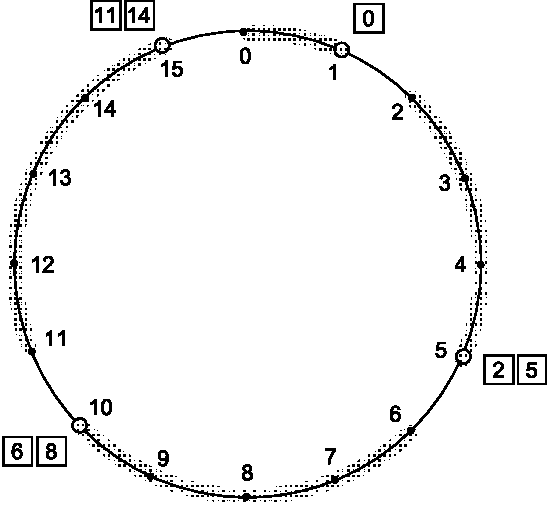
\includegraphics[width=0.4\textwidth]{pictures/pic0}\\
  \caption[Example of a $4$-bit Chord identifier circle]{Example of a $4$-bit Chord identifier circle.
  The responsibility ranges for each peer are accentuated in light gray}\label{fig:pic0}
\end{figure}
Es lassen sich auch mehrere Bilder nebeneinander platzieren wie z.B. in Abbildung
\ref{fig:multipic} zu sehen ist.
\begin{figure}[hpbt]
 \centering
  %%----start of first subfigure----
  \subfloat[FIFO size limited to 20 entries]{
   \label{fig:multipic:a} %% label for first subfigure
   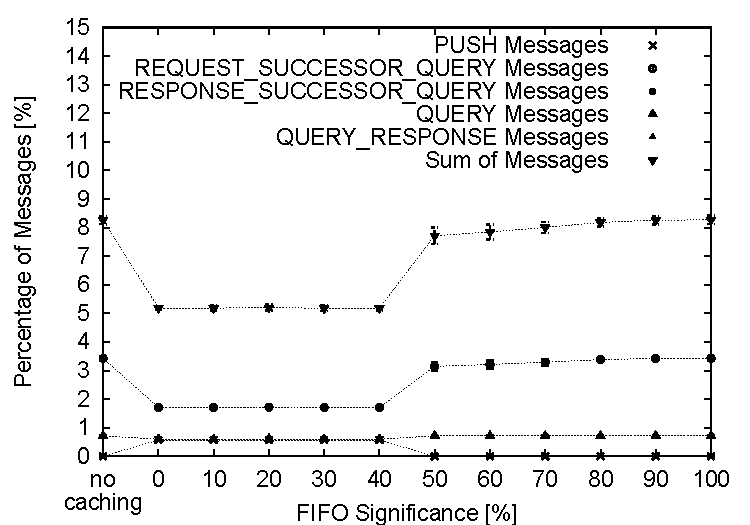
\includegraphics[width=0.48\linewidth]{pic1}}
  \hspace{0.01\textwidth}
  %%----start of second subfigure----
  \subfloat[FIFO size limited to 30 entries]{
   \label{fig:multipic:b} %% label for second subfigure
   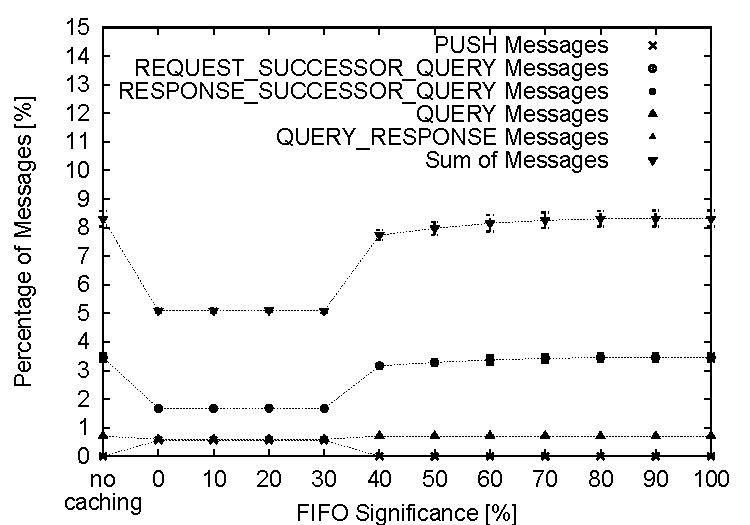
\includegraphics[width=0.48\linewidth]{pic2}}\\[0pt] % horizontal break
  %%----start of third subfigure----
  \subfloat[FIFO size limited to 40 entries]{
   \label{fig:multipic:c} %% label for third subfigure
   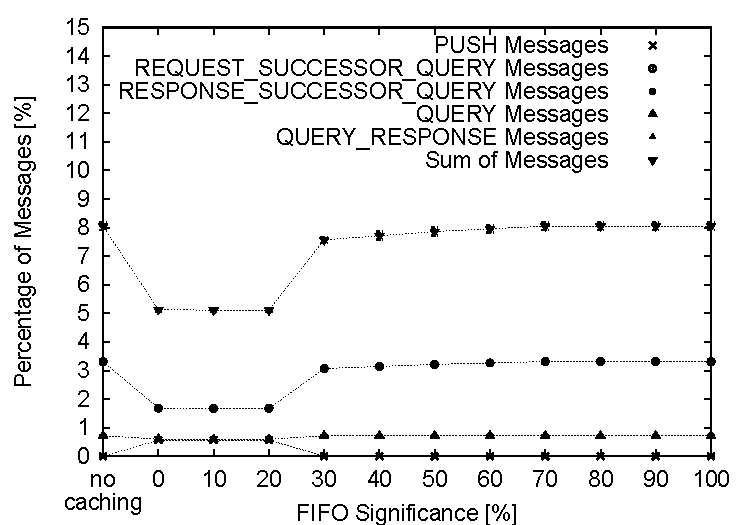
\includegraphics[width=0.48\linewidth]{pic3}}
  \hspace{0.01\textwidth}
  %%----start of fourth subfigure----
  \subfloat[FIFO size limited to 50 entries]{
   \label{fig:multipic:d} %% label for fourth subfigure
   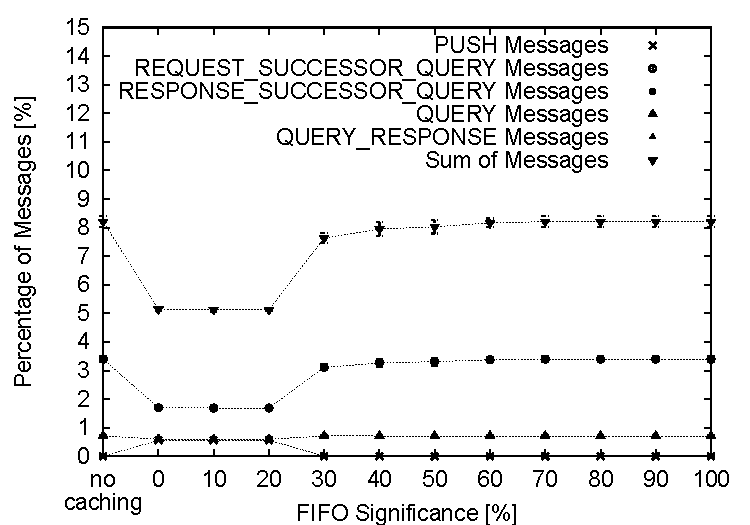
\includegraphics[width=0.48\linewidth]{pic4}}
 \caption[Observed message fractions and 95\% confidence intervals for Chord]{Observed message fractions and 95\% confidence intervals for Chord without the influence of churn. The FIFO capacity varies from 20 (\ref{fig:multipic:a}) -- 50 (\ref{fig:multipic:d}) entries (decadic steps).}
 \label{fig:multipic} %% label for entire figure
\end{figure}

\subsection{Programm Code}
Eine elegante M�glichkeit, Programmtext einzubinden, l�sst sich mit dem listings-Paket erreichen.
Das \verb|HelloWorld| Programm aus Listing \ref{lst:hw} hat in Zeile \ref{line:hw3} �brigens einen Programmierfehler.
\begin{lstlisting}[float=htp,caption=Hello World,label=lst:hw,language=Java, numbers=left, numberstyle=\tiny, stepnumber=2, numbersep=8pt, escapeinside={//@}{@//},backgroundcolor=\color{yellow},xleftmargin=3ex,xrightmargin=1ex]
public class HelloWorld {
    public static void main(String[] args) {
        Syste.out.println("Hello, World"); //@\label{line:hw3}@//
    }
}
\end{lstlisting}

\subsection{Fu�noten}
Wenn man auf Google \footnote{\url{http://www.google.com}} verweisen will, bietet sich statt einer gesonderten
Referenz auch einfach eine Fu�note an.
\subsection{Formeln}
Man kann mit \LaTeX\ sehr sch�n Formeln erzeugen:
$$L_{P}(k) = R^{orig}_{P}(k) + \sum_{i=0}^n 2*R^{i}_{P}(k)$$

% further chapters
%
% =================================================================================================
% place your appendix here
% -------------------------------------------------------------------------------------------------
%
\appendix
% -------------------------------------------------------------------------------------------------
%      MDSG Latex Framework
%      ============================================================================================
%      File:                  appendix.tex
%      Author(s):             Michael Duerr
%      Version:               1
%      Creation Date:         30. Mai 2010
%      Creation Date:         30. Mai 2010
%
%      Notes:                 - Place your appendix here
%                             - Use the same commands (`chapter', `section', ...) as in main text
% -------------------------------------------------------------------------------------------------
%
\chapter{Training Parameters}\label{ax:training_params}
\small{
    \begin{verbatim}
required arguments:
  --algo ALGO           Algorithm to use for training. Choose between 'ppo'
                        and 'dqn'.

optional arguments:
  -h, --help            show this help message and exit
  --seed SEED           Generate the same set of pseudo random constellations,
                        colors, positions, etc. every time the algorithm is
                        executed. (default: 1)
  --agents AGENTS       Amount of agents. (default: 2)
  --model MODEL         Path of the model inside the storage folder, if none
                        is given then a random name is generated. (default:
                        None)
  --capture CAPTURE     Boolean to enable capturing of the environment. The
                        outcome are in form of gifs. (default: True)
  --env ENV             Environment ID, choose between Empty-Grid-v0 for an
                        empty environment and FourRooms-Grid-v0 for an
                        environment divided into equal sized rooms. (default:
                        Empty-Grid-v0)
  --agent-view-size AGENT_VIEW_SIZE
                        Grid size the agent can see. Agent Observation is
                        based on that field of view. For example, 7x7 grid
                        size means agent can see three tiles in each
                        direction. (default: 7)
  --grid-size GRID_SIZE
                        Size of the environment grid. (default: 5)
  --max-steps MAX_STEPS
                        Maximum amount of steps an agent has to reach a goal.
                        If none is given then this max count is set to: grid
                        size * grid size. (default: None)
  --setting SETTING     Setting can be either: '' for cooperation, 'mixed-
                        motive' for a mixed motive environment, 'mixed-motive-
                        competitive' for a competitive composition or
                        'difference-reward' for a setting that calculates
                        difference rewards. Cooperation means all agents get
                        the same reward. If set to mixed-motive or mixed-
                        motive-competitve the reward is not shared and each
                        agent is responsible for its own success. In
                        competitive mode, agents can take over opponent
                        coloration without resetting the cells, otherwise
                        cells are always reset when colored and walked over.
                        The last option 'difference-reward' is a cooperation
                        setting but calculates the reward for each agent by
                        subtracting a new reward from the total reward. The
                        new reward just excludes the action of this one agent.
                        A high difference reward means, that the action of
                        that agent was good. (default: '' for cooperation)
  --market MARKET       There are three options: 'sm', 'am' and '' for none.
                        SM = Shareholder Market where agents can sell or buy
                        shares on the market. AM = Action Market where agents
                        can buy specific actions from others. (default = '')
  --trading-fee TRADING_FEE
                        If a market transaction is executed, this value
                        determines the price, i.e. in an action market this
                        defines the price the buyer pays. In a shareholder
                        market this value defines the share value. (default:
                        0.1)
  --frames FRAMES       Number of frames of training. (default: 80.000)
  --frames-per-proc FRAMES_PER_PROC
                        Number of frames per process. In case of PPO this is
                        the number of steps, before the model is optimized.
                        (default: 128)
  --procs PROCS         Number of processes/environments running parallel.
                        (default: 16)
  --recurrence RECURRENCE
                        Number of time-steps the gradient is back propagated.
                        If it is greater than one, a LSTM is added to the
                        model to have memory. (default: 1)
  --batch-size BATCH_SIZE
                        Batch size that is used for sampling. (default: 64)
  --gamma GAMMA         Discount factor with 0 <= gamma < 1, specify how
                        important future estimated rewards are. High value
                        means high importance. (default: 0.99)
  --log-interval LOG_INTERVAL
                        Number of frames between two logs. (default: 1)
  --save-interval SAVE_INTERVAL
                        Number of times the --frames-per-proc amount of frames
                        needs to be reached, to log the current training
                        values, i.e. rewards, into a csv file. (default: 10, 0
                        means no saving)
  --capture-interval CAPTURE_INTERVAL
                        Number of times --frames-per-proc amount of frames
                        needs to be reached, to capture the last --capture-
                        frames amount of steps into a gif. Warning: --capture
                        needs to be set to True as well. (default: 10, 0 means
                        no capturing)
  --capture-frames CAPTURE_FRAMES
                        Number of frames that are captured. (default: 50, 0
                        means no capturing)
  --lr LR               Learning rate. (default: 0.001)
  --optim-eps OPTIM_EPS
                        Epsilon value for the Adam optimizer. (default: 1e-8)
  --epochs EPOCHS       [PPO] Number of epochs for PPO optimization. (default:
                        4)
  --gae-lambda GAE_LAMBDA
                        [PPO] Lambda coefficient in GAE formula, used for
                        calculation of the advantage values. (default: 0.95, 1
                        means no gae)
  --entropy-coef ENTROPY_COEF
                        [PPO] Entropy term coefficient. (default: 0.01)
  --value-loss-coef VALUE_LOSS_COEF
                        [PPO] Value loss term coefficient. (default: 0.5)
  --max-grad-norm MAX_GRAD_NORM
                        [PPO] Maximum norm of gradient. (default: 0.5)
  --clip-eps CLIP_EPS   [PPO] Clipping epsilon for PPO. (default: 0.2)
  --epsilon-start EPSILON_START
                        [DQN] Starting value of epsilon, used for action
                        selection. (default: 1.0 -> high exploration)
  --epsilon-end EPSILON_END
                        [DQN] Ending value of epsilon, used for action
                        selection. (default: 0.01 -> high exploitation)
  --epsilon-decay EPSILON_DECAY
                        [DQN] Controls the rate of the epsilon decay in order
                        to shift from exploration to exploitation. The higher
                        the value the slower epsilon decays. (default: 5.000)
  --replay-size REPLAY_SIZE
                        [DQN] Size of the replay memory. (default: 40.000)
  --initial-target-update INITIAL_TARGET_UPDATE
                        [DQN] Frames until the target network is updated,
                        Needs to be smaller than --target-update! (default:
                        1.000)
  --target-update TARGET_UPDATE
                        [DQN] Frames between updating the target network,
                        Needs to be smaller or equal to --frames-per-proc and
                        bigger than --initial-target-update! (default: 15.000)
    \end{verbatim}
}


\chapter{Detailed Results}\label{ax:plots}

\subsection{Easy Environment}
The following plots show all details of the best training results in a small 5x5 grid. The default parameters of Appendix \ref{ax:training_params} are used for all executions. Only the agent amount, setting and market value change. In the first Figure \ref{fig:ax-easy-1}, one agent is acting in the environment, all other trainings are executed with two agents. For details see Chapter \ref{sec:Results}. An example to run a training process is shown below.

\begin{lstlisting}[float=htp,language=bash, escapeinside={//@}{@//},xleftmargin=3ex,xrightmargin=1ex]
$ python -m scripts.train
    --algo ppo
    --model ppo-easy
    --agents 2
\end{lstlisting}

\newpage
\vfill
% [!hpbt]
\begin{figure}
    \centering
    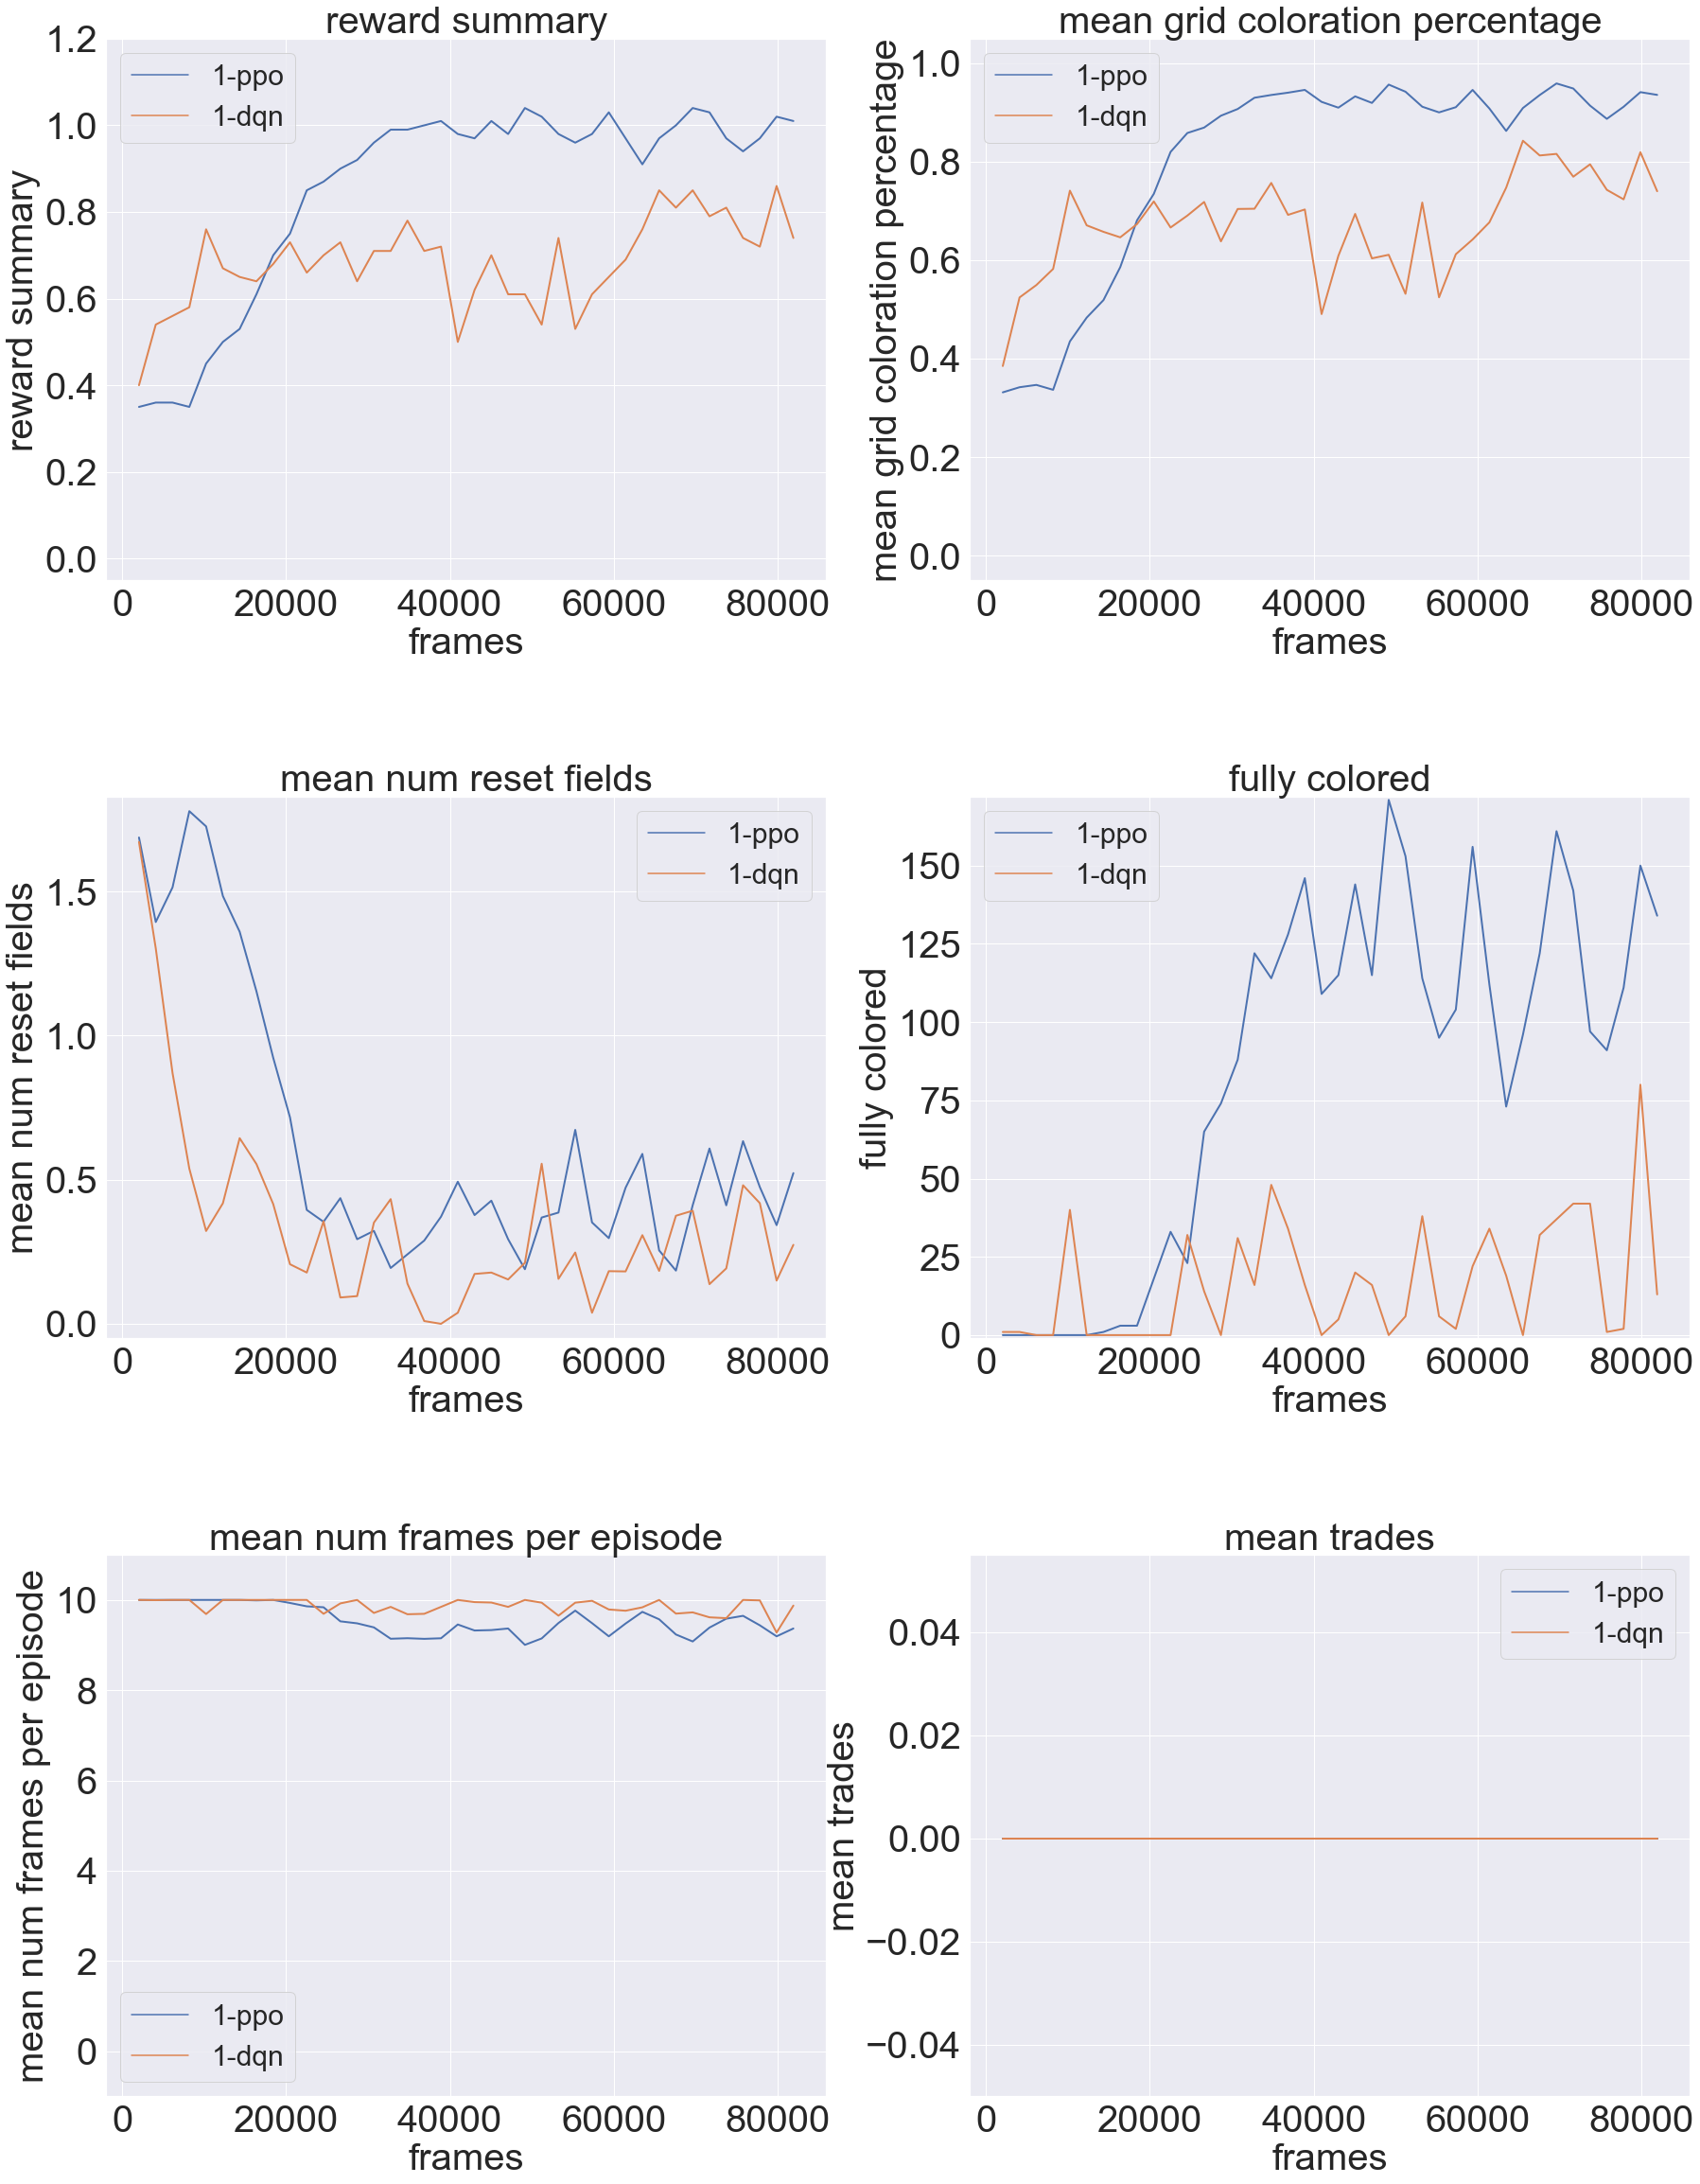
\includegraphics[width=1\textwidth]{AX-easy-1.png}\\
    \caption[PPO and DQN Training Details with One Agent]{Details of the training with one agent using PPO and DQN}\label{fig:ax-easy-1}
\end{figure}
\vfill
\clearpage


\newpage
\vfill
\begin{figure}
    \centering
    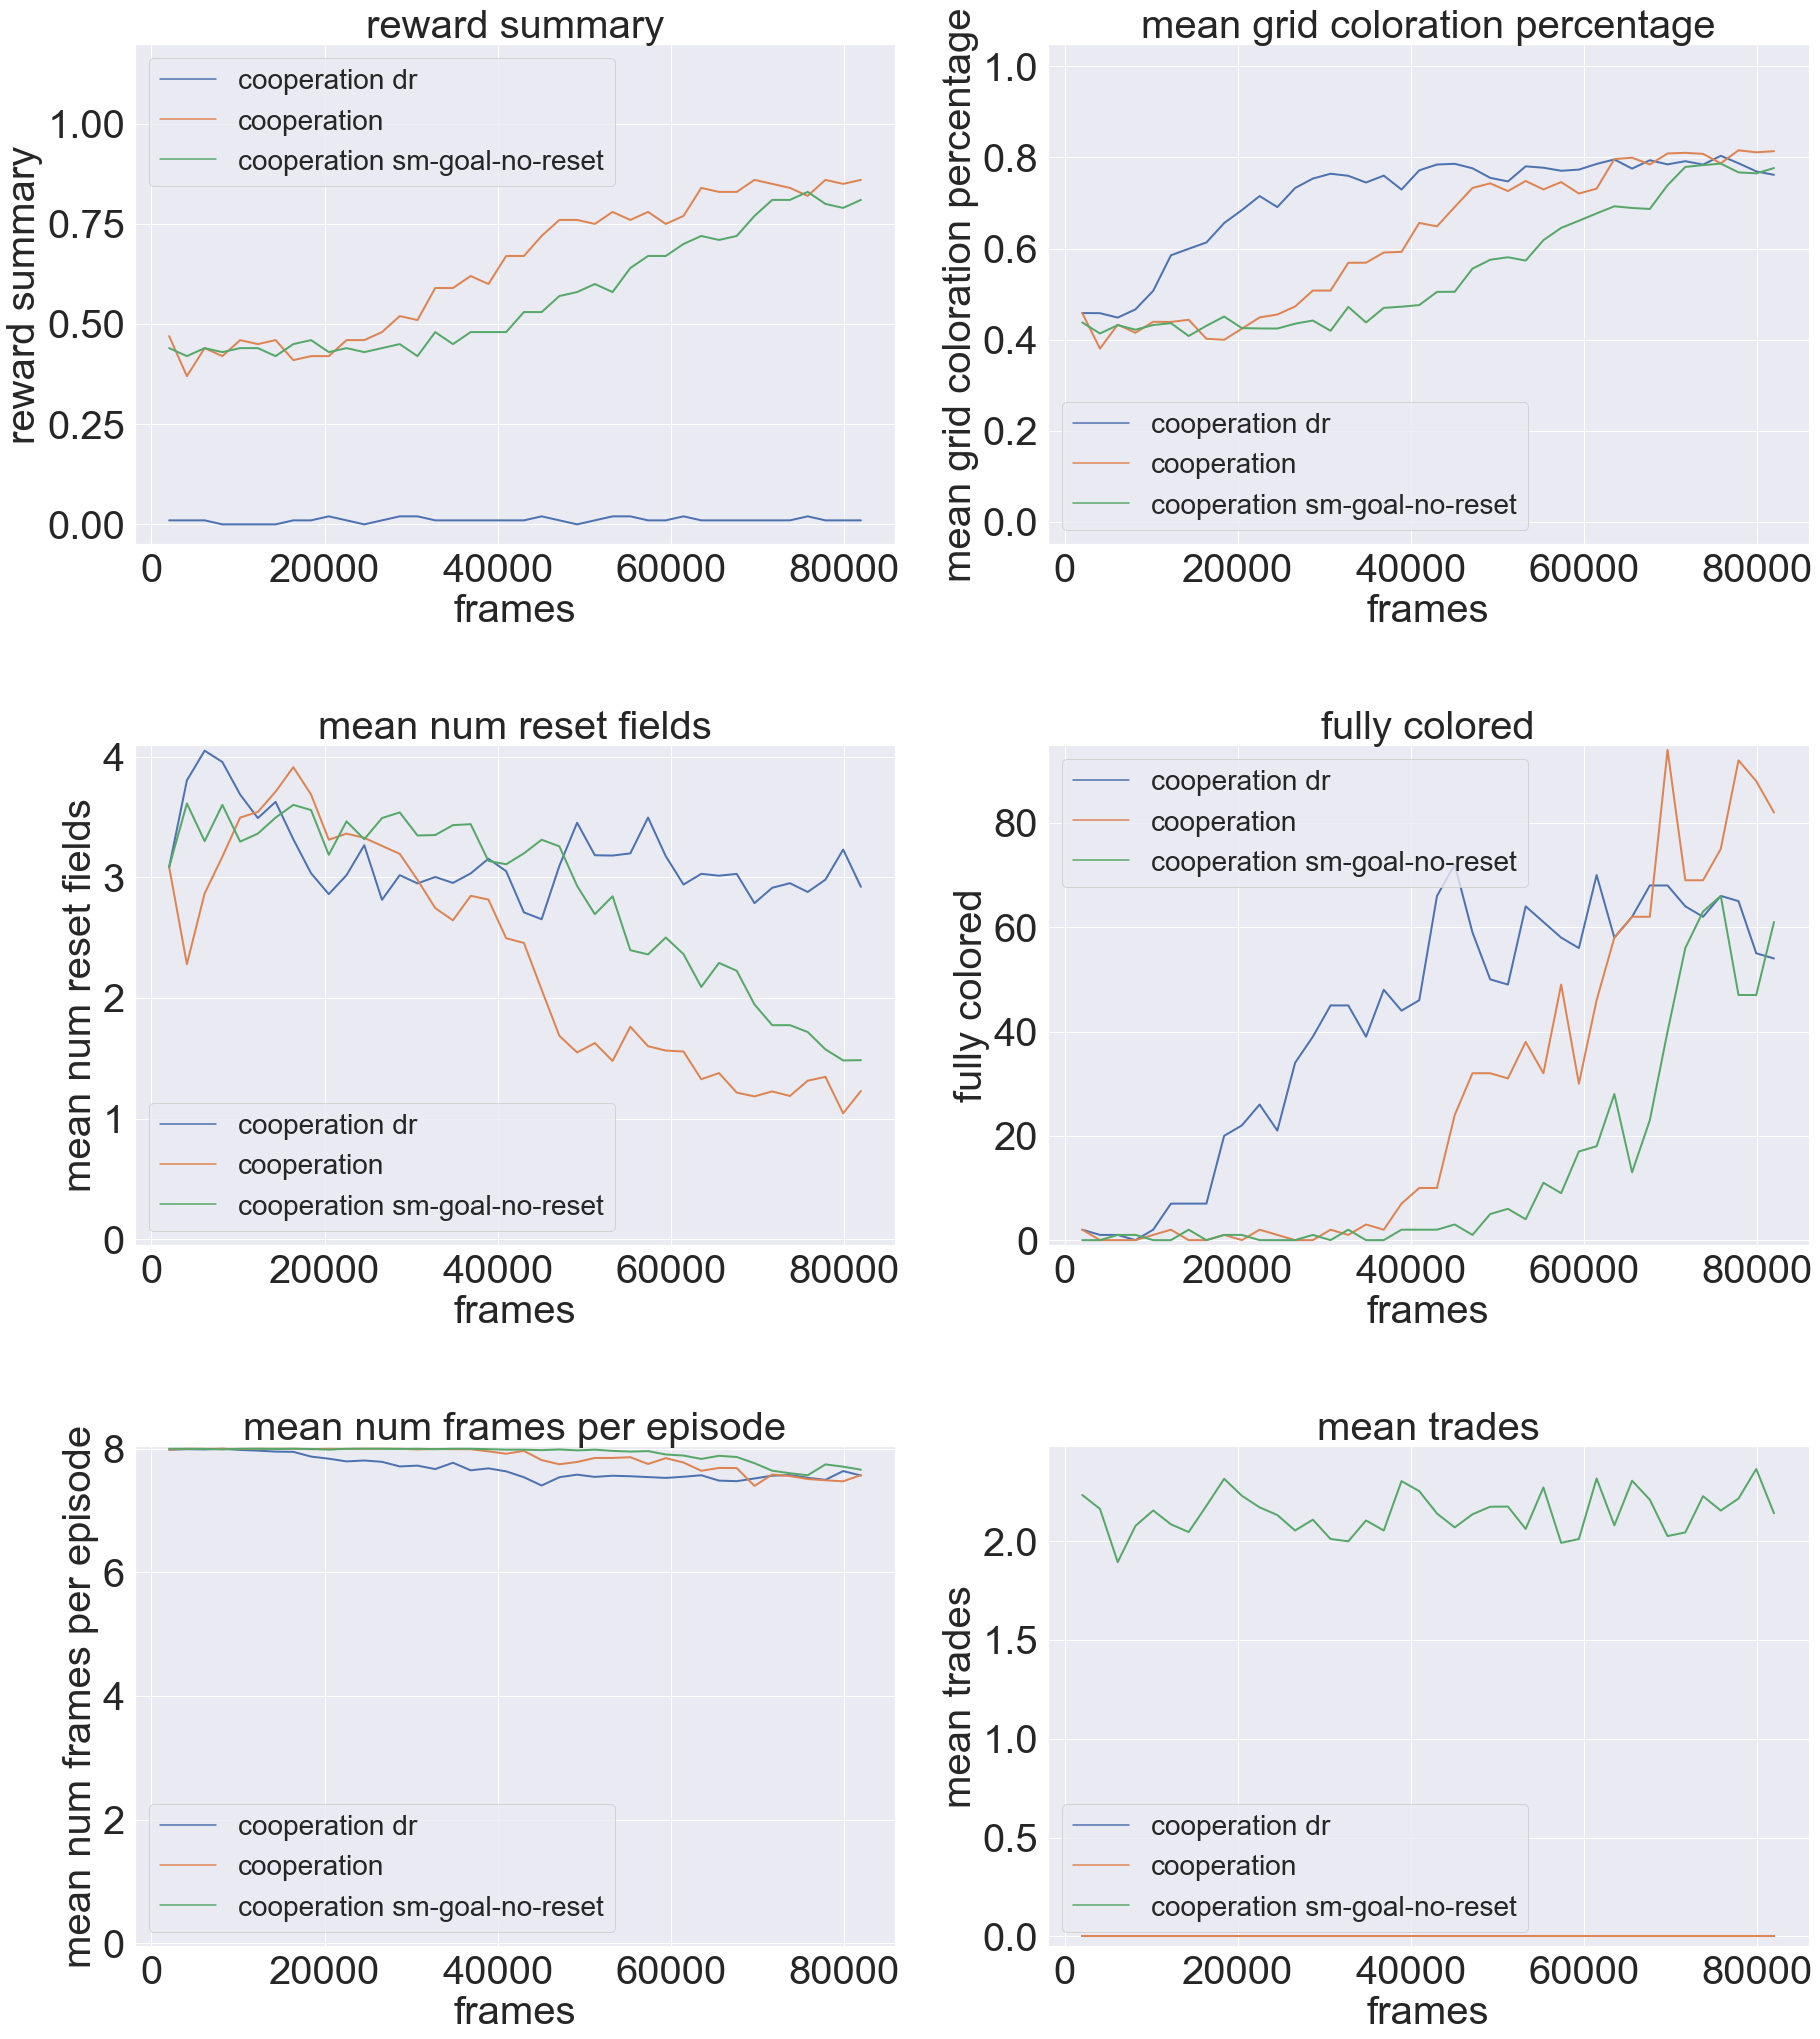
\includegraphics[width=1\textwidth]{AX-easy-2-ppo-coop.png}\\
    \caption[Training Details of Top PPO Cooperation Executions]{Top cooperation score details of two PPO agents}\label{fig:ax-easy-2-ppo-coop}
\end{figure}
\vfill
\clearpage


\newpage
\vfill
\begin{figure}
    \centering
    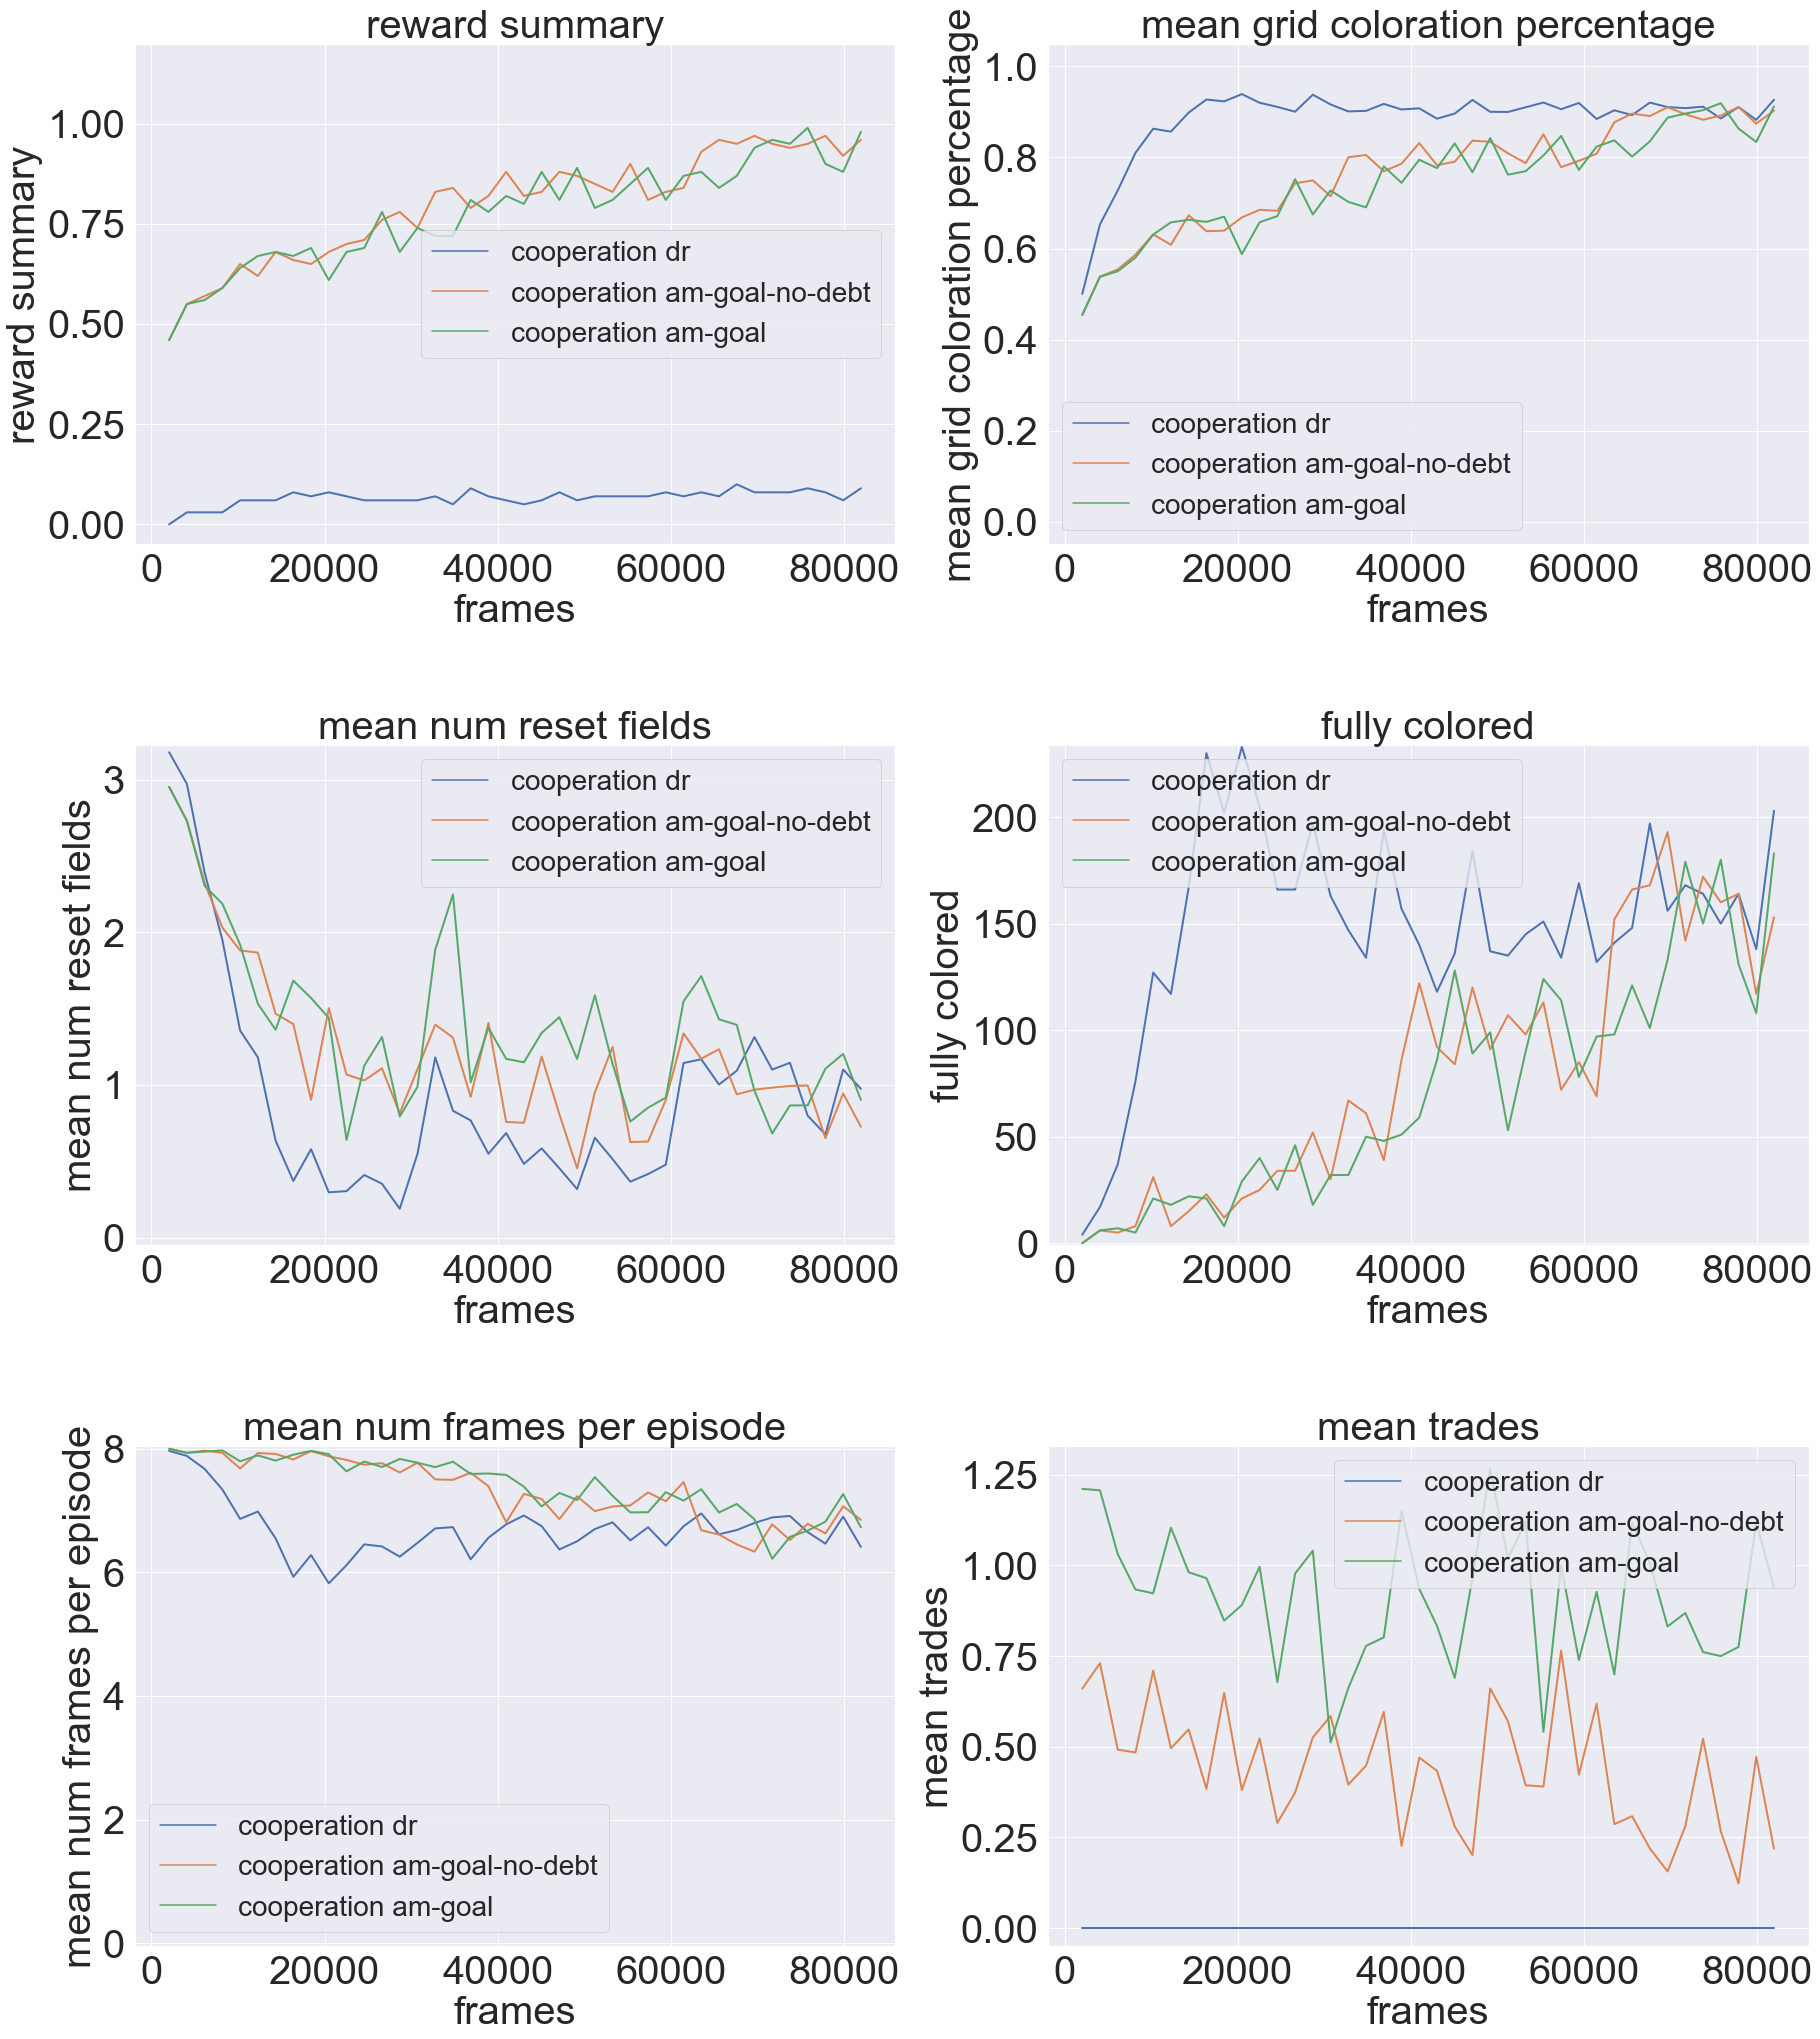
\includegraphics[width=1\textwidth]{AX-easy-2-dqn-coop.png}\\
    \caption[Training Details of Top DQN Cooperation Executions]{Top cooperation score details of two DQN agents}\label{fig:ax-easy-2-dqn-coop}
\end{figure}
\vfill
\clearpage


\newpage
\vfill
\begin{figure}
    \centering
    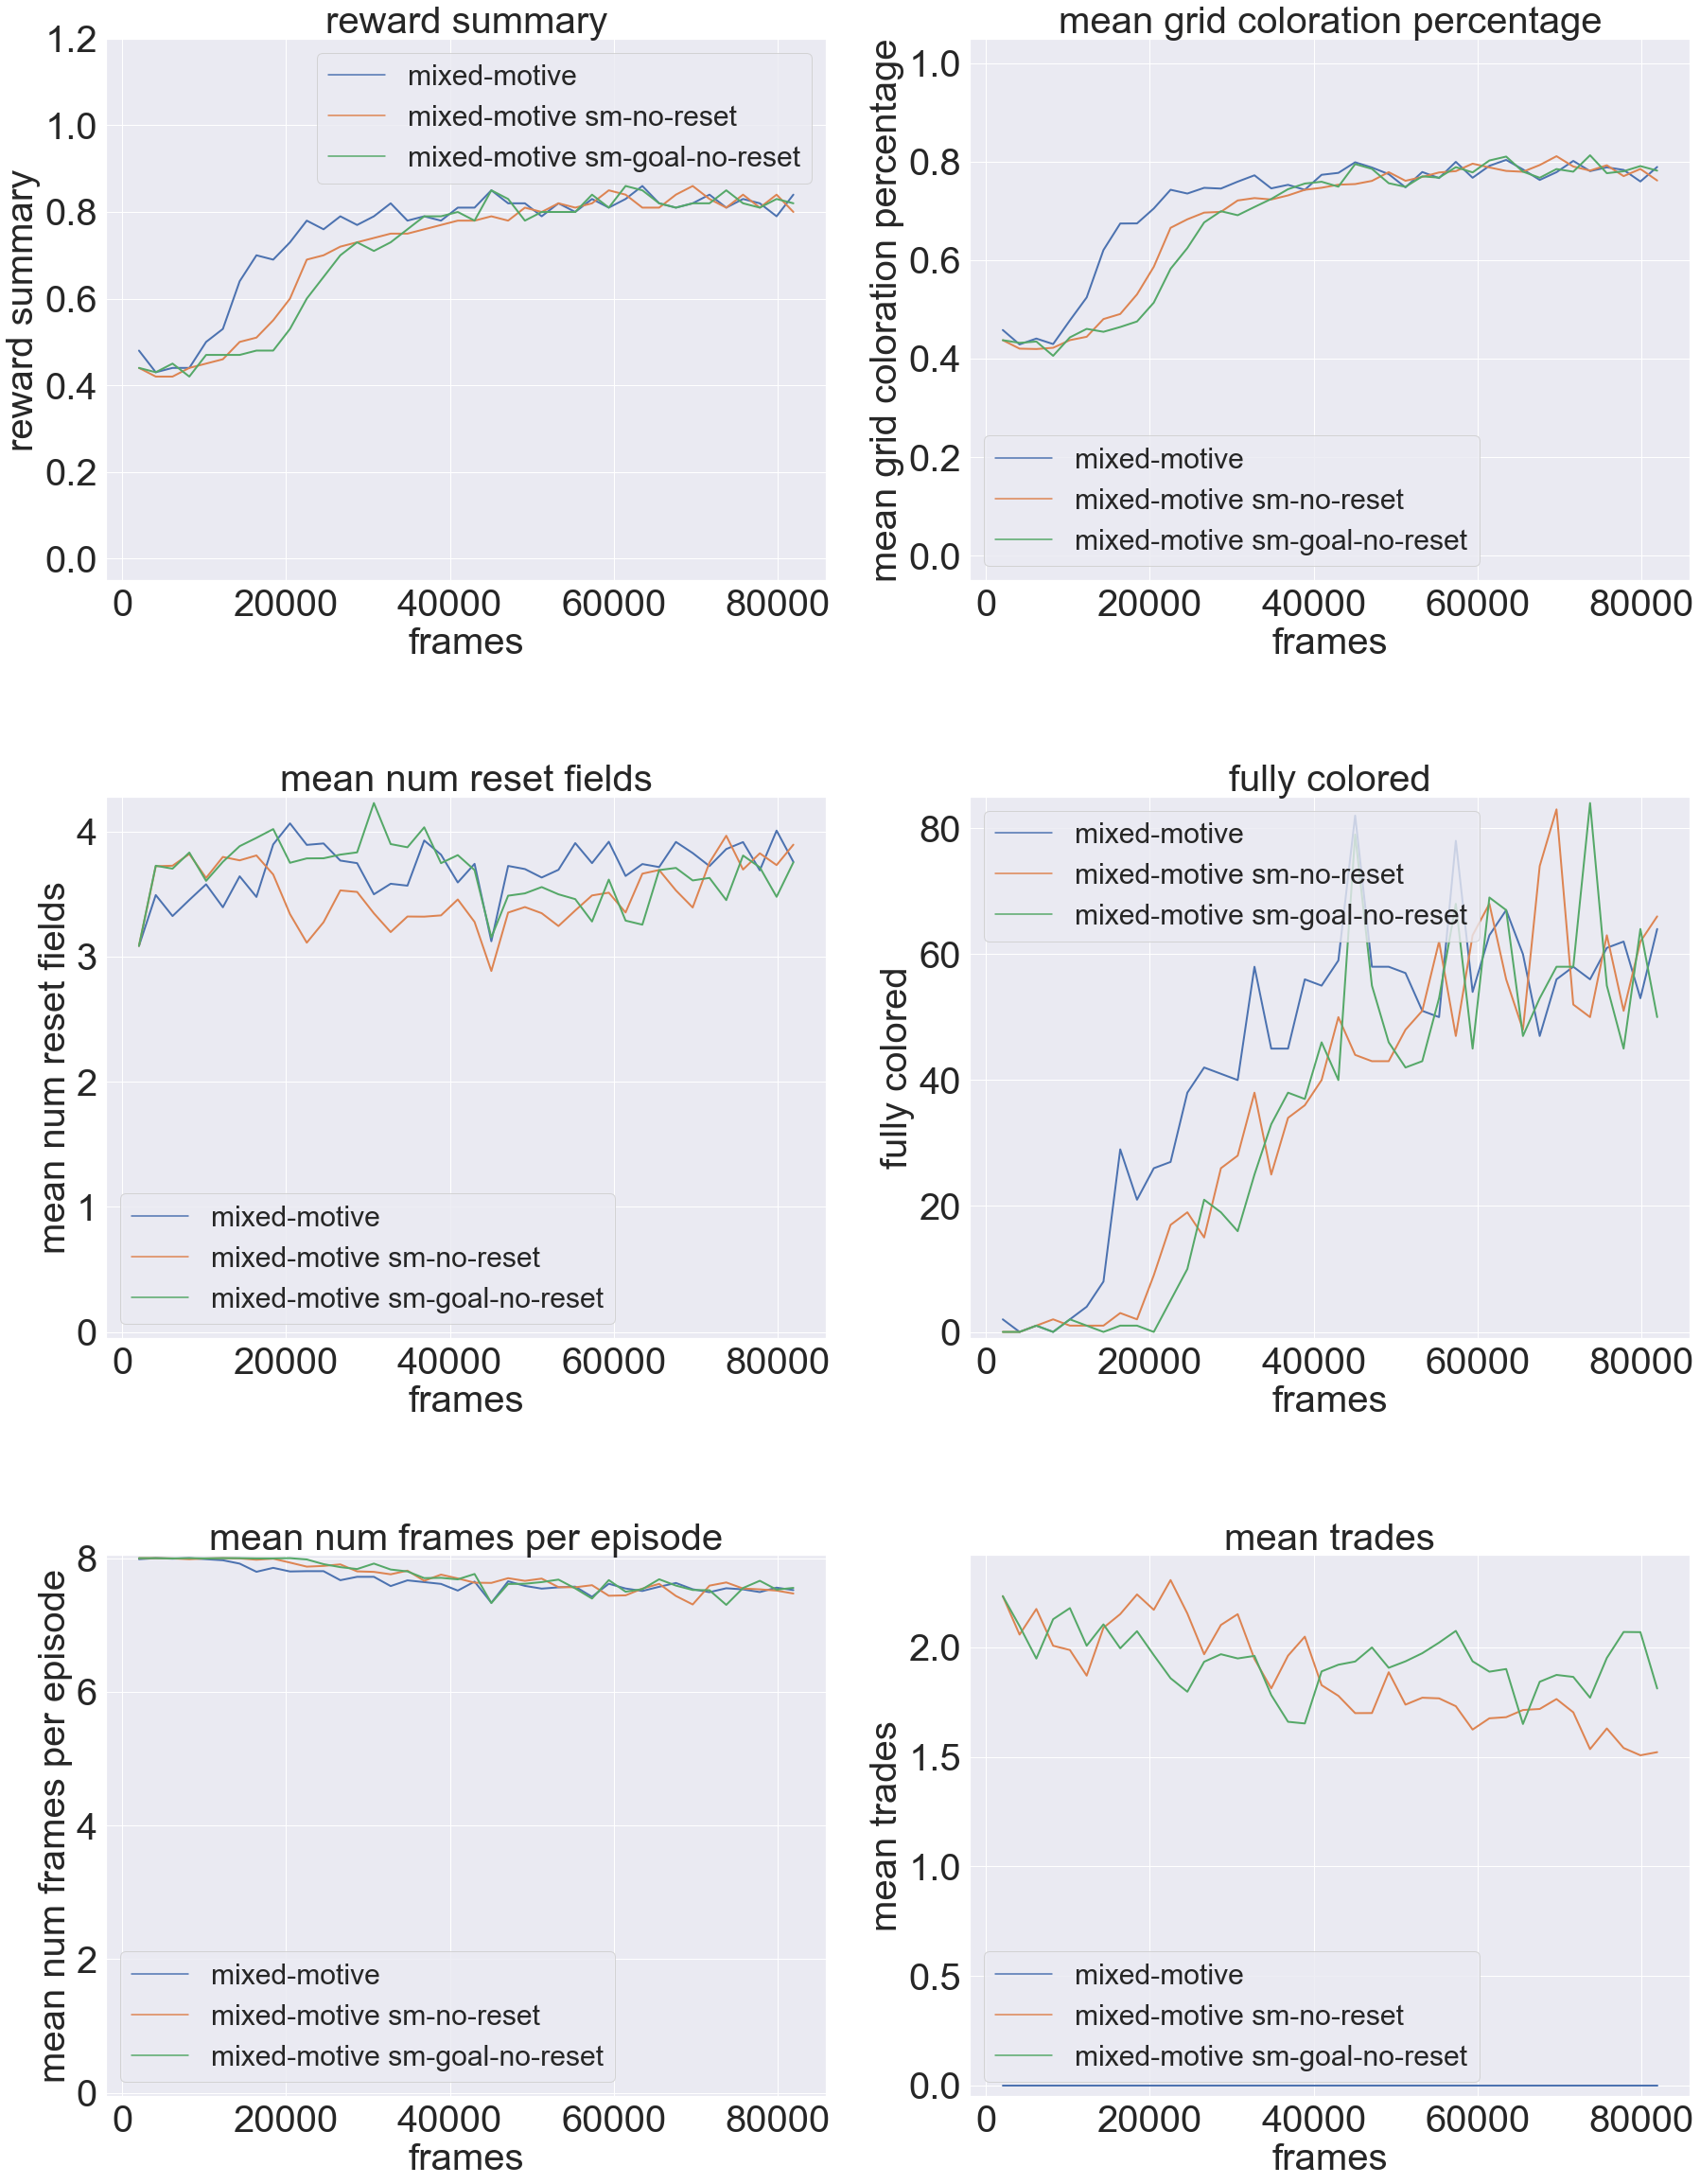
\includegraphics[width=1\textwidth]{AX-easy-2-ppo-mixed.png}\\
    \caption[Training Details of Top PPO Mixed-Motive Executions]{Top mixed-motive score details of two PPO agents}\label{fig:ax-easy-2-ppo-mixed}
\end{figure}
\vfill
\clearpage


\newpage
\vfill
\begin{figure}
    \centering
    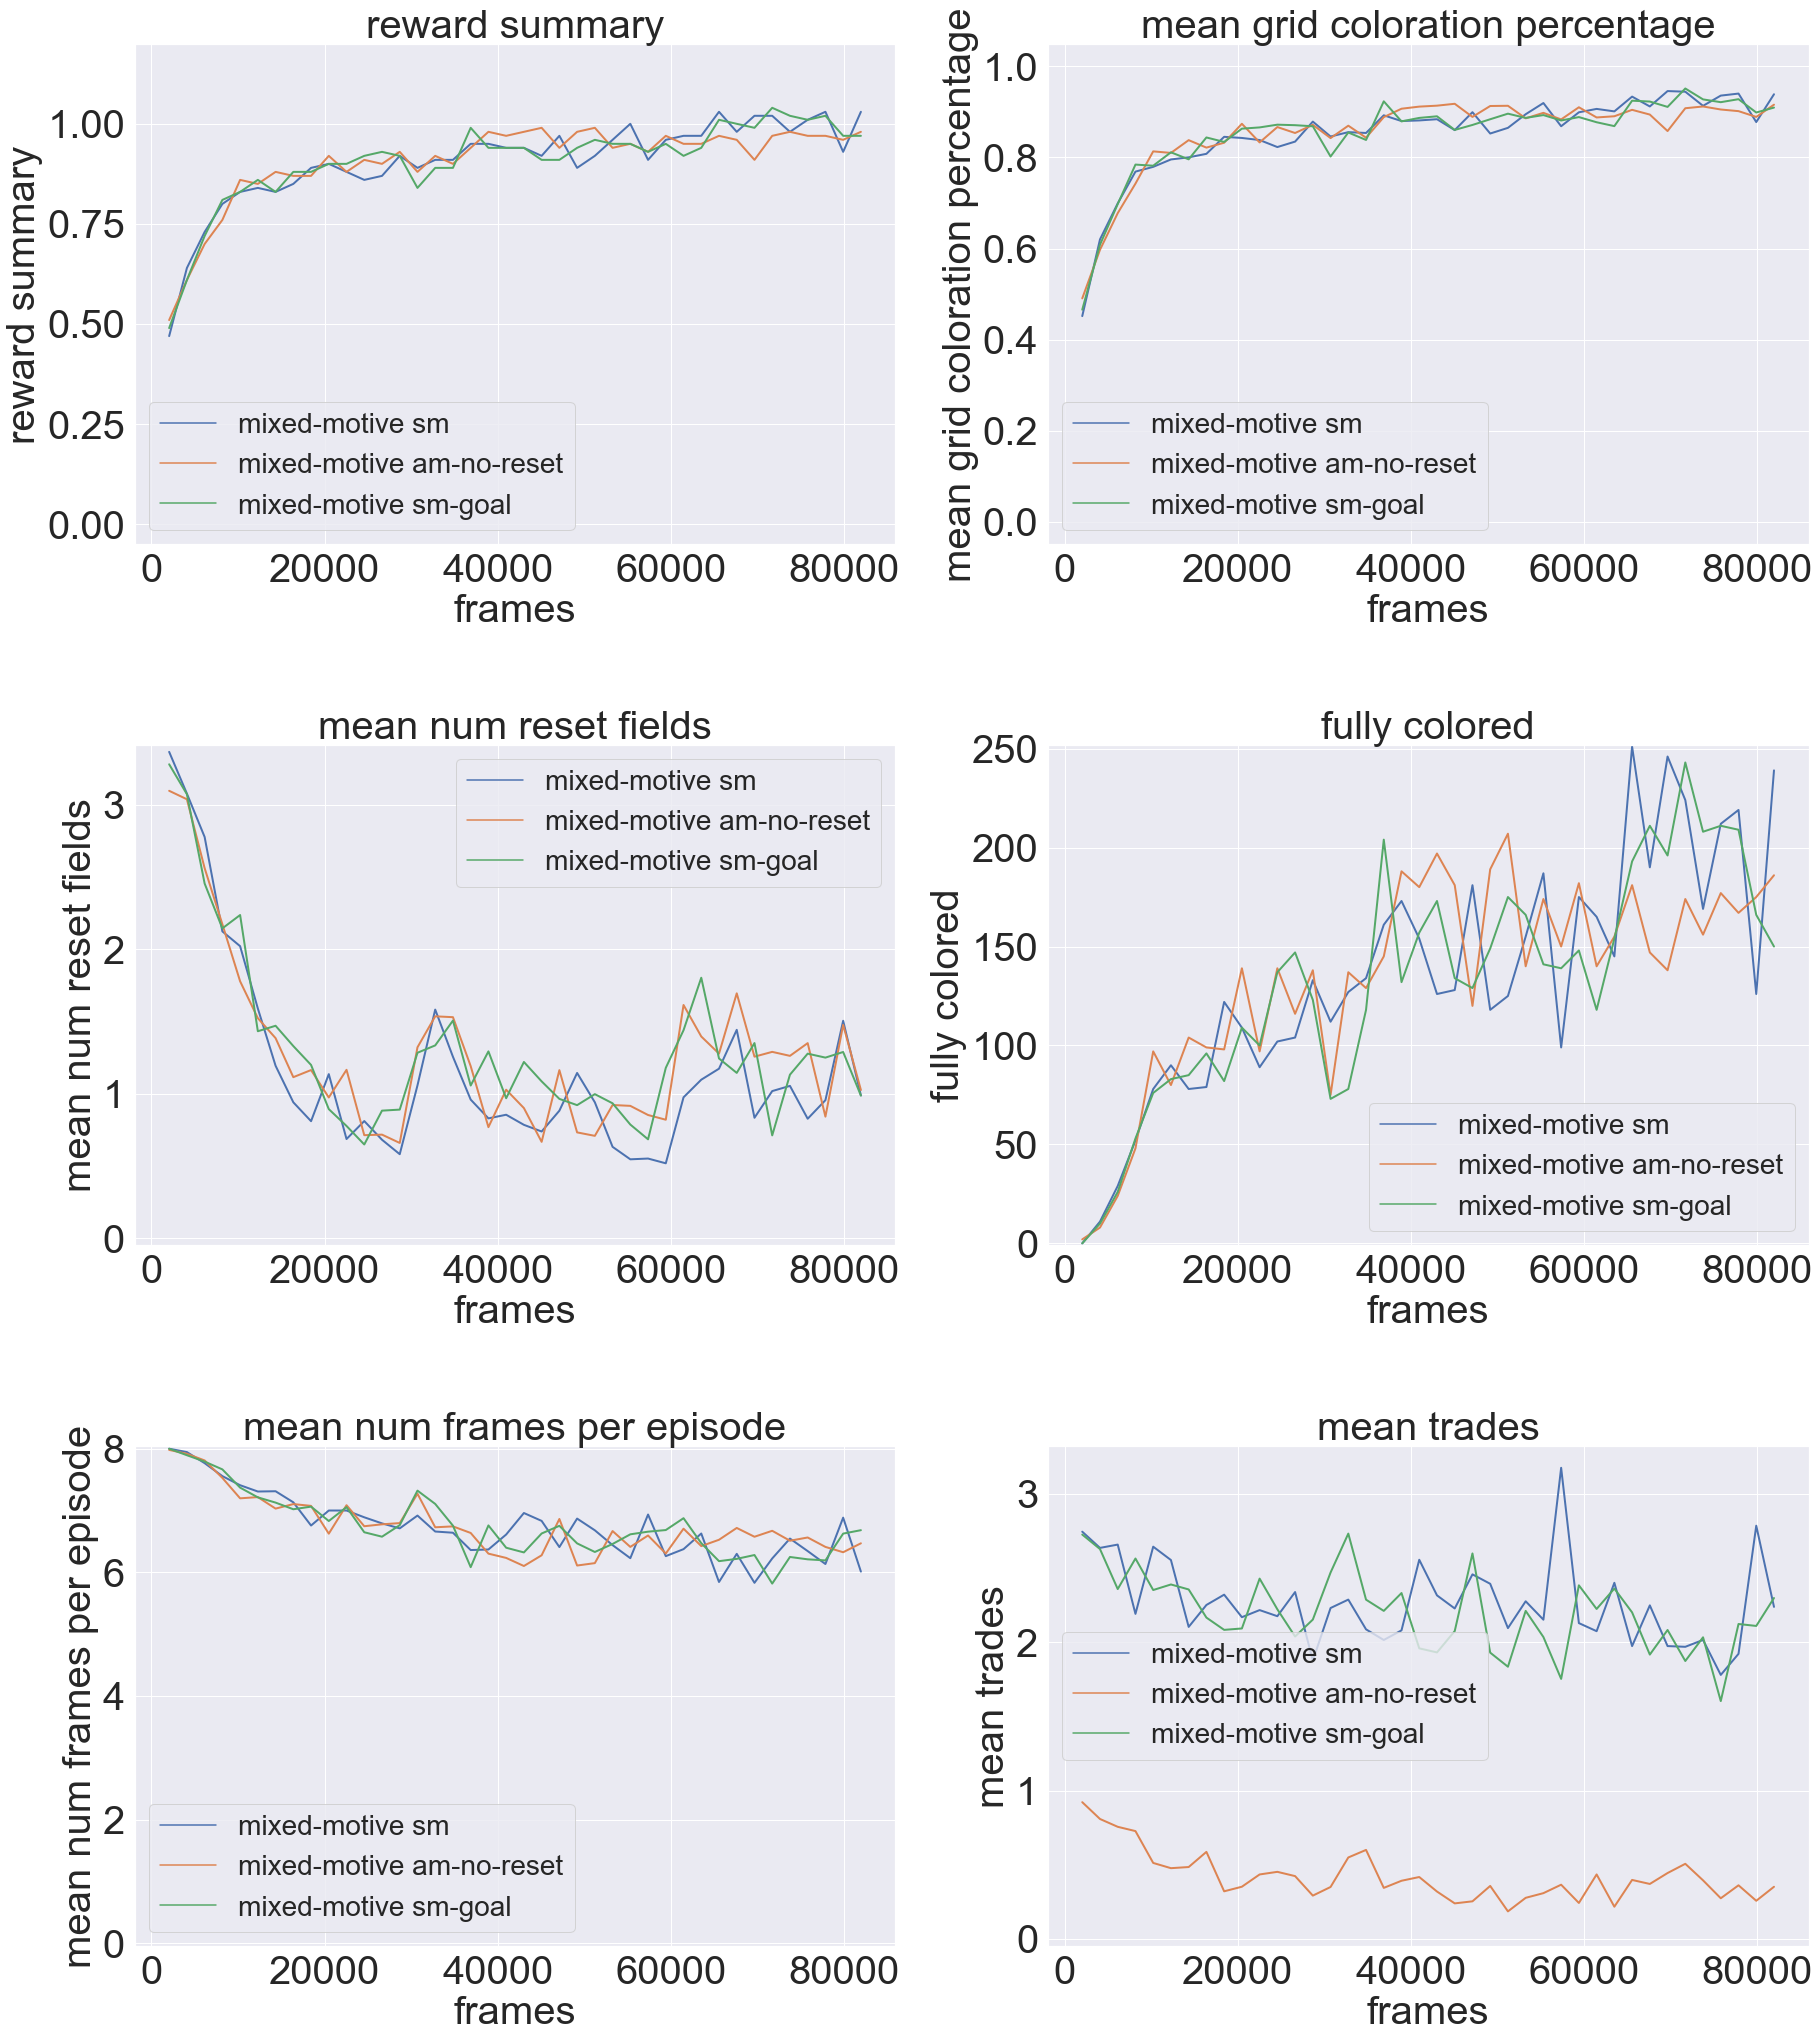
\includegraphics[width=1\textwidth]{AX-easy-2-dqn-mixed.png}\\
    \caption[Training Details of Top DQN Mixed-Motive Executions]{Top mixed-motive score details of two DQN agents}\label{fig:ax-easy-2-dqn-mixed}
\end{figure}
\vfill
\clearpage


\newpage
\vfill
\begin{figure}
    \centering
    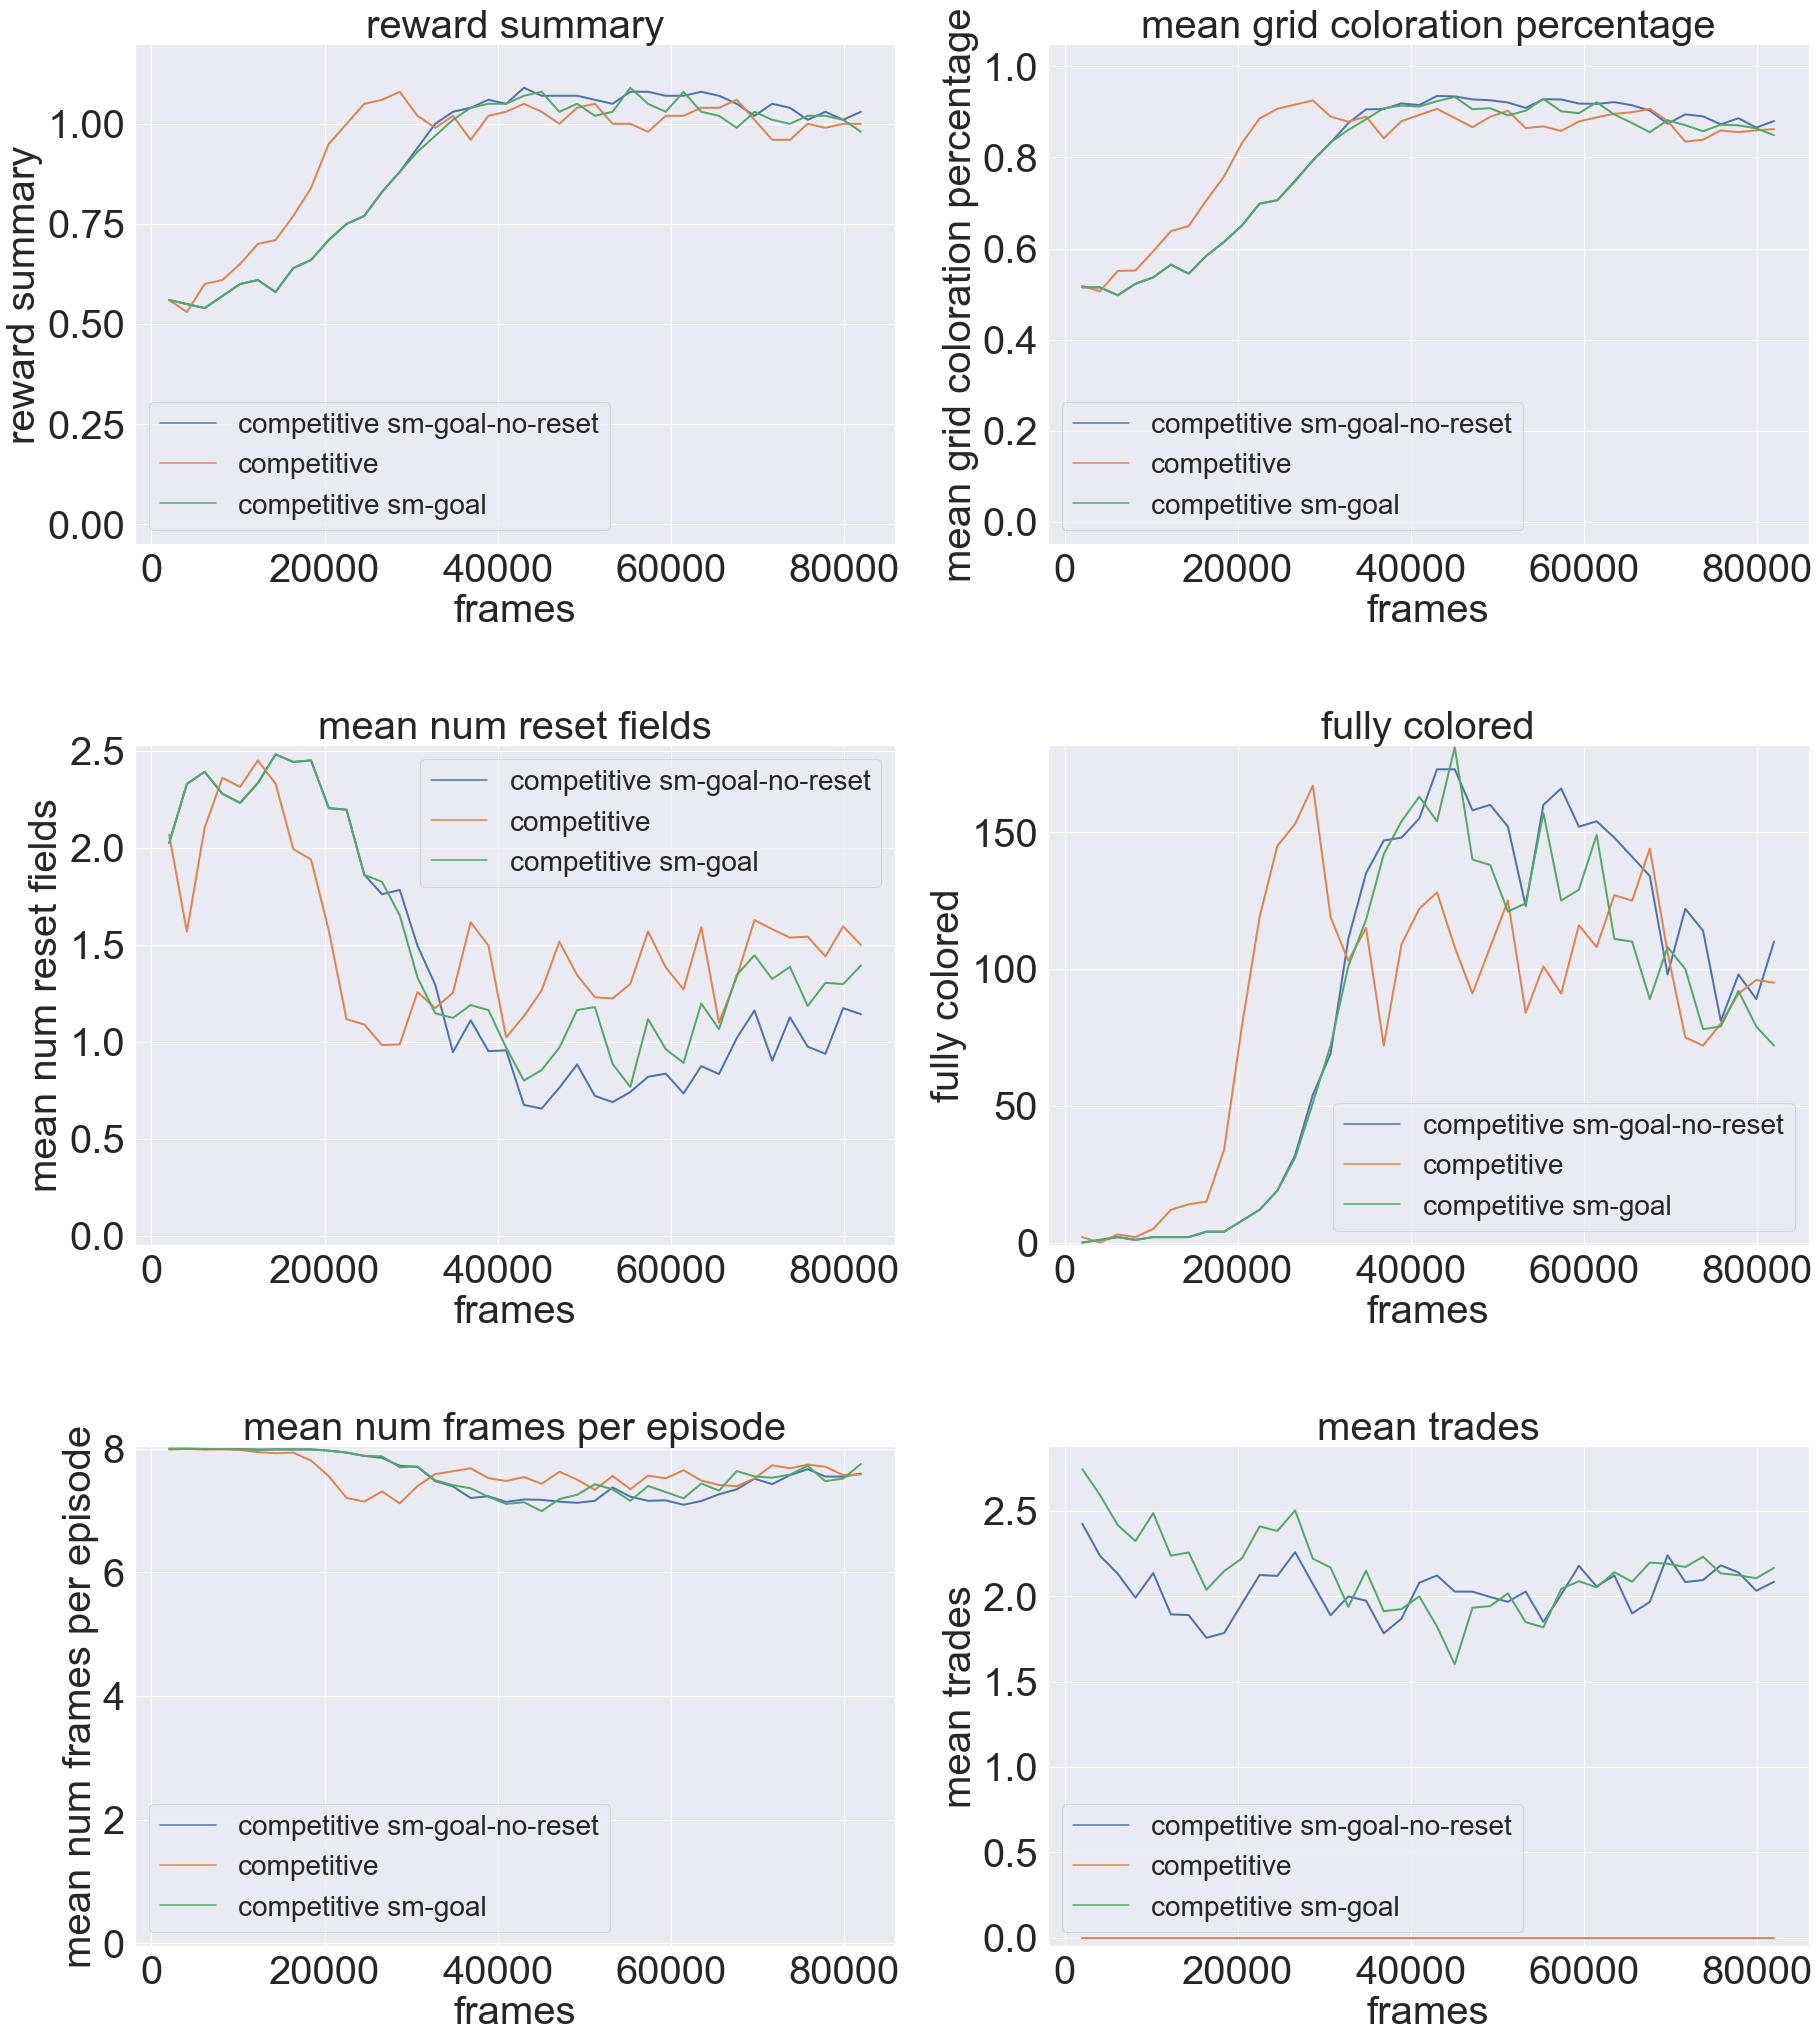
\includegraphics[width=1\textwidth]{AX-easy-2-ppo-comp.png}\\
    \caption[Training Details of Top PPO Competitive Executions]{Top competitive score details of two PPO agents}\label{fig:ax-easy-2-ppo-comp}
\end{figure}
\vfill
\clearpage


\newpage
\vfill
\begin{figure}
    \centering
    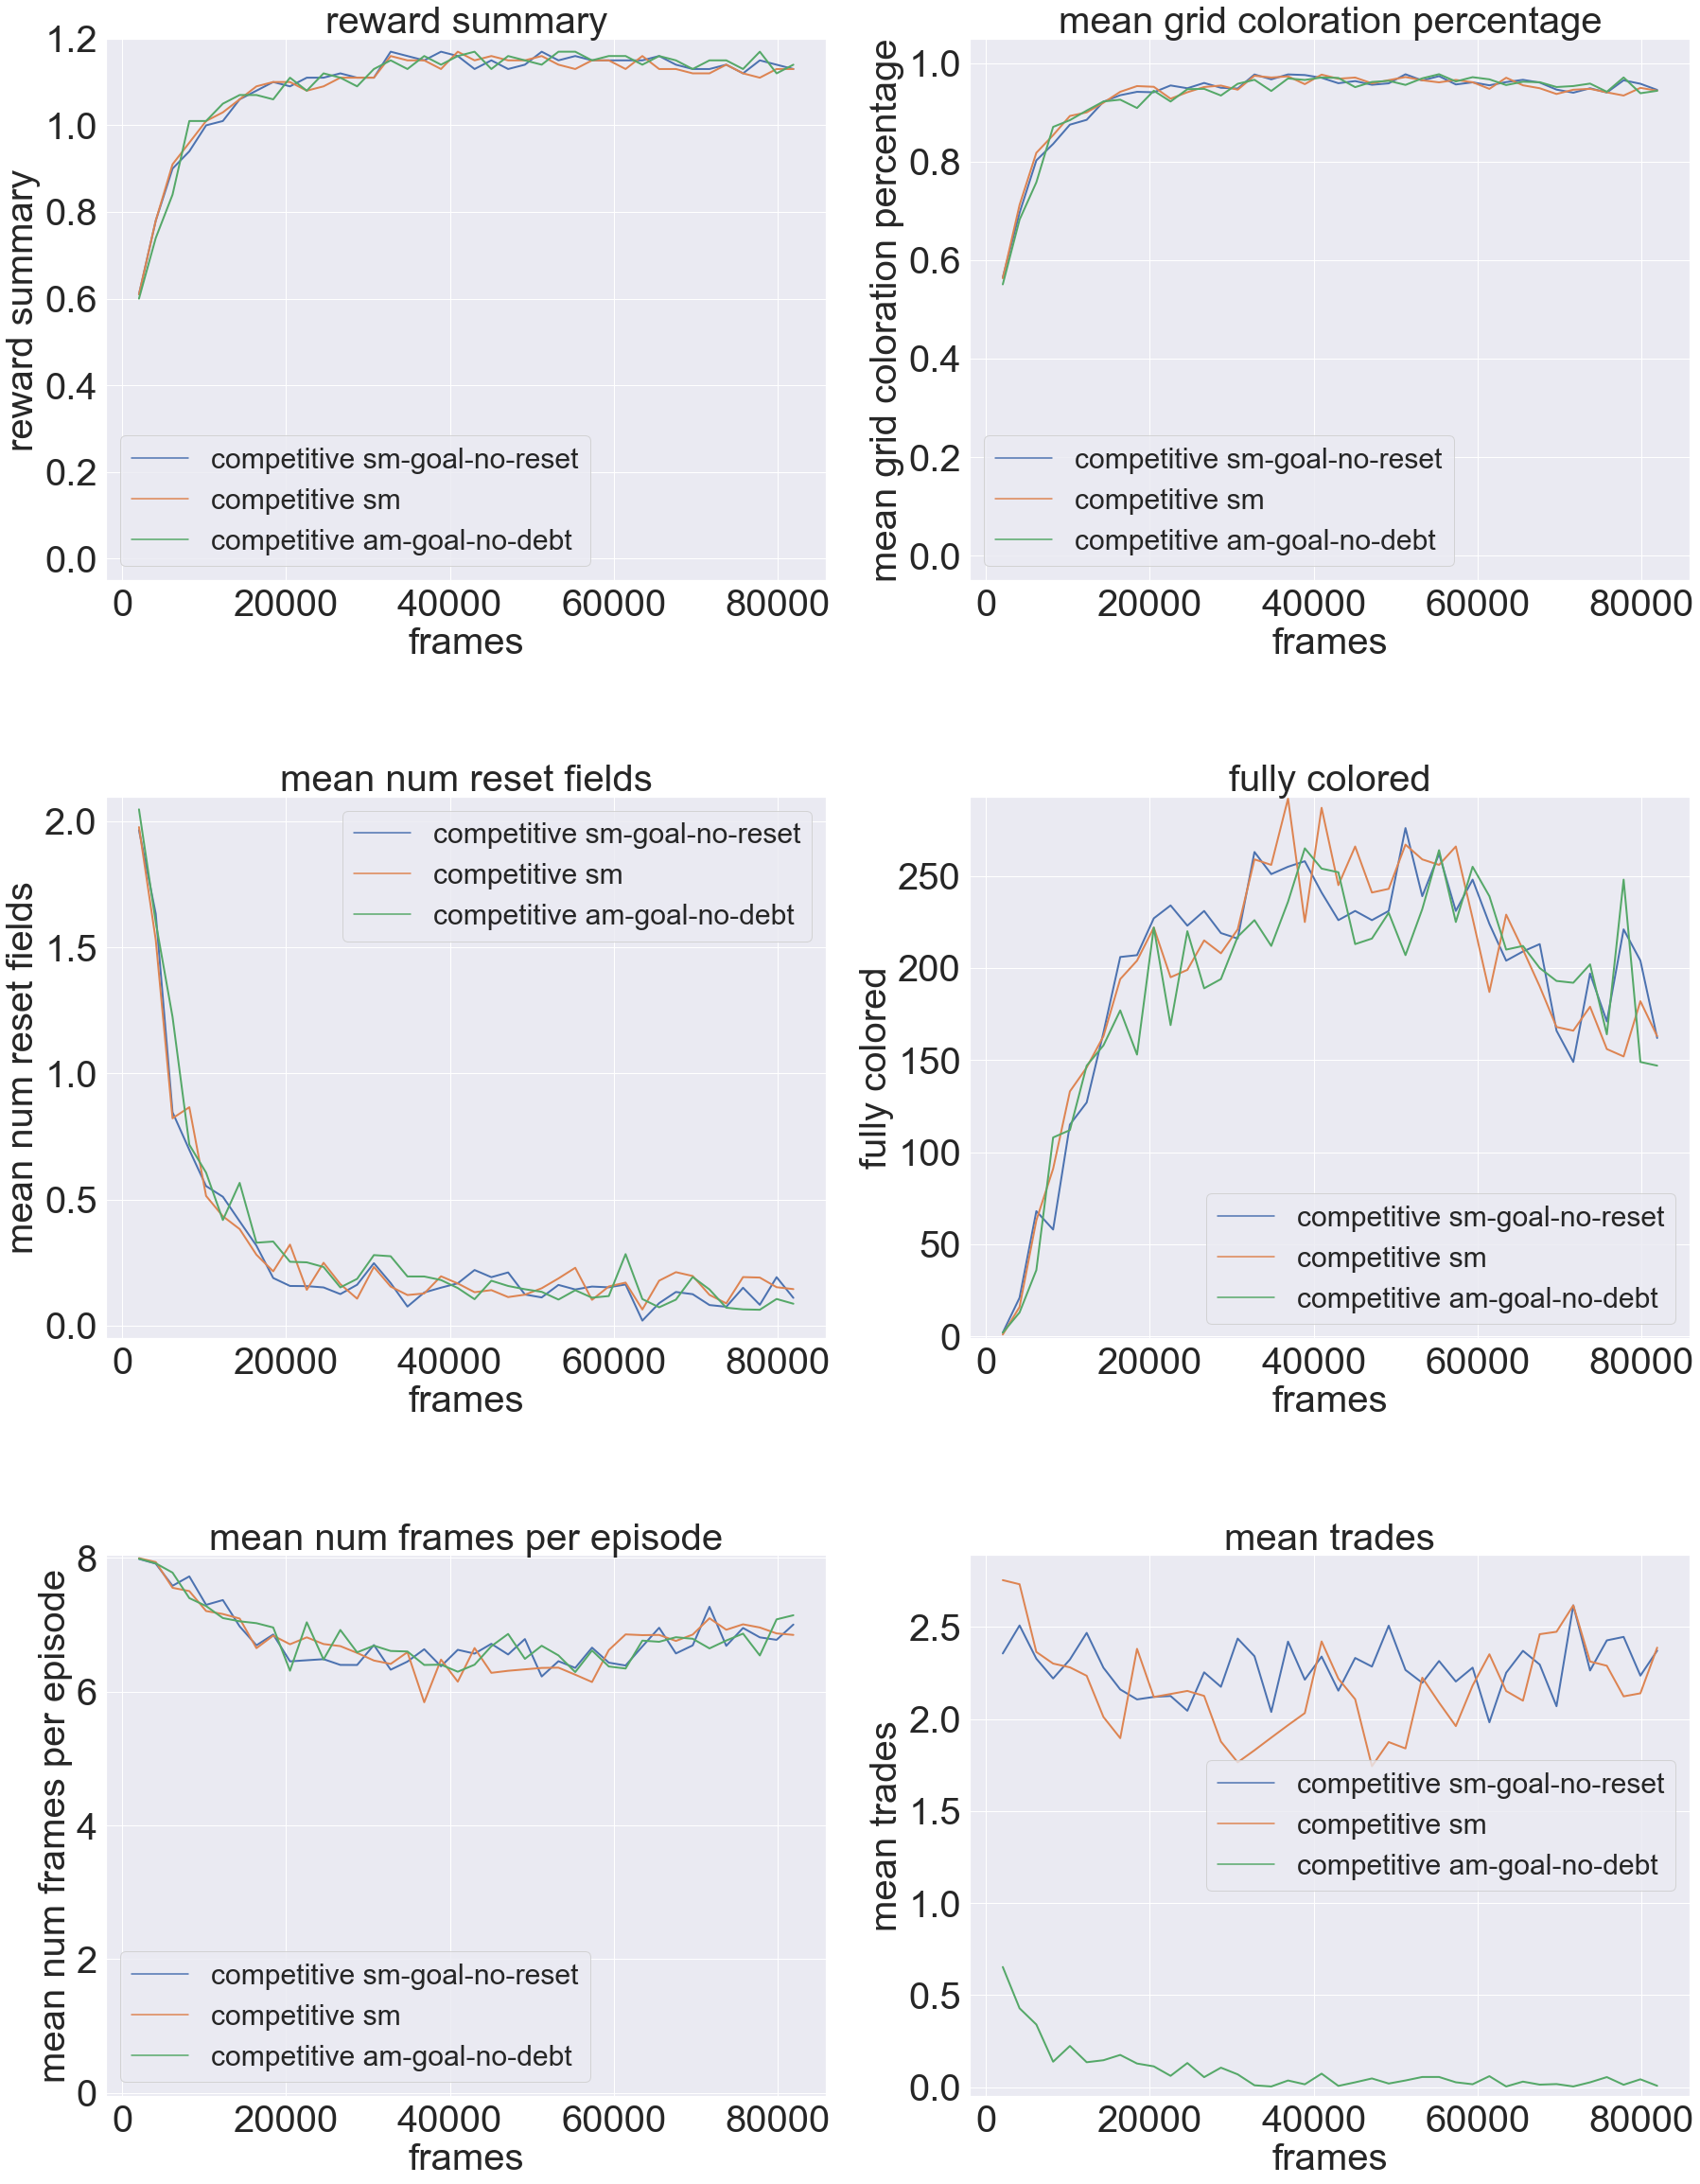
\includegraphics[width=1\textwidth]{AX-easy-2-dqn-comp.png}\\
    \caption[Training Details of Top DQN Competitive Executions]{Top competitive score details of two DQN agents}\label{fig:ax-easy-2-dqn-comp}
\end{figure}
\vfill
\clearpage

\subsection{Difficult Environment}
An example to run a training process in a seven by seven environment is shown below.

\begin{lstlisting}[float=htp,language=bash, escapeinside={//@}{@//},xleftmargin=3ex,xrightmargin=1ex]
$ python -m scripts.train 
    --algo dqn 
    --model dqn-difficult
    --agents 3
    --target-update 10000 
    --replay-size 700000 
    --epsilon-decay 20000
    --grid-size 7 
    --max-steps 20 
    --frames-per-proc 256
    --frames 200000
\end{lstlisting}

\newpage
\vfill
\begin{figure}
    \centering
    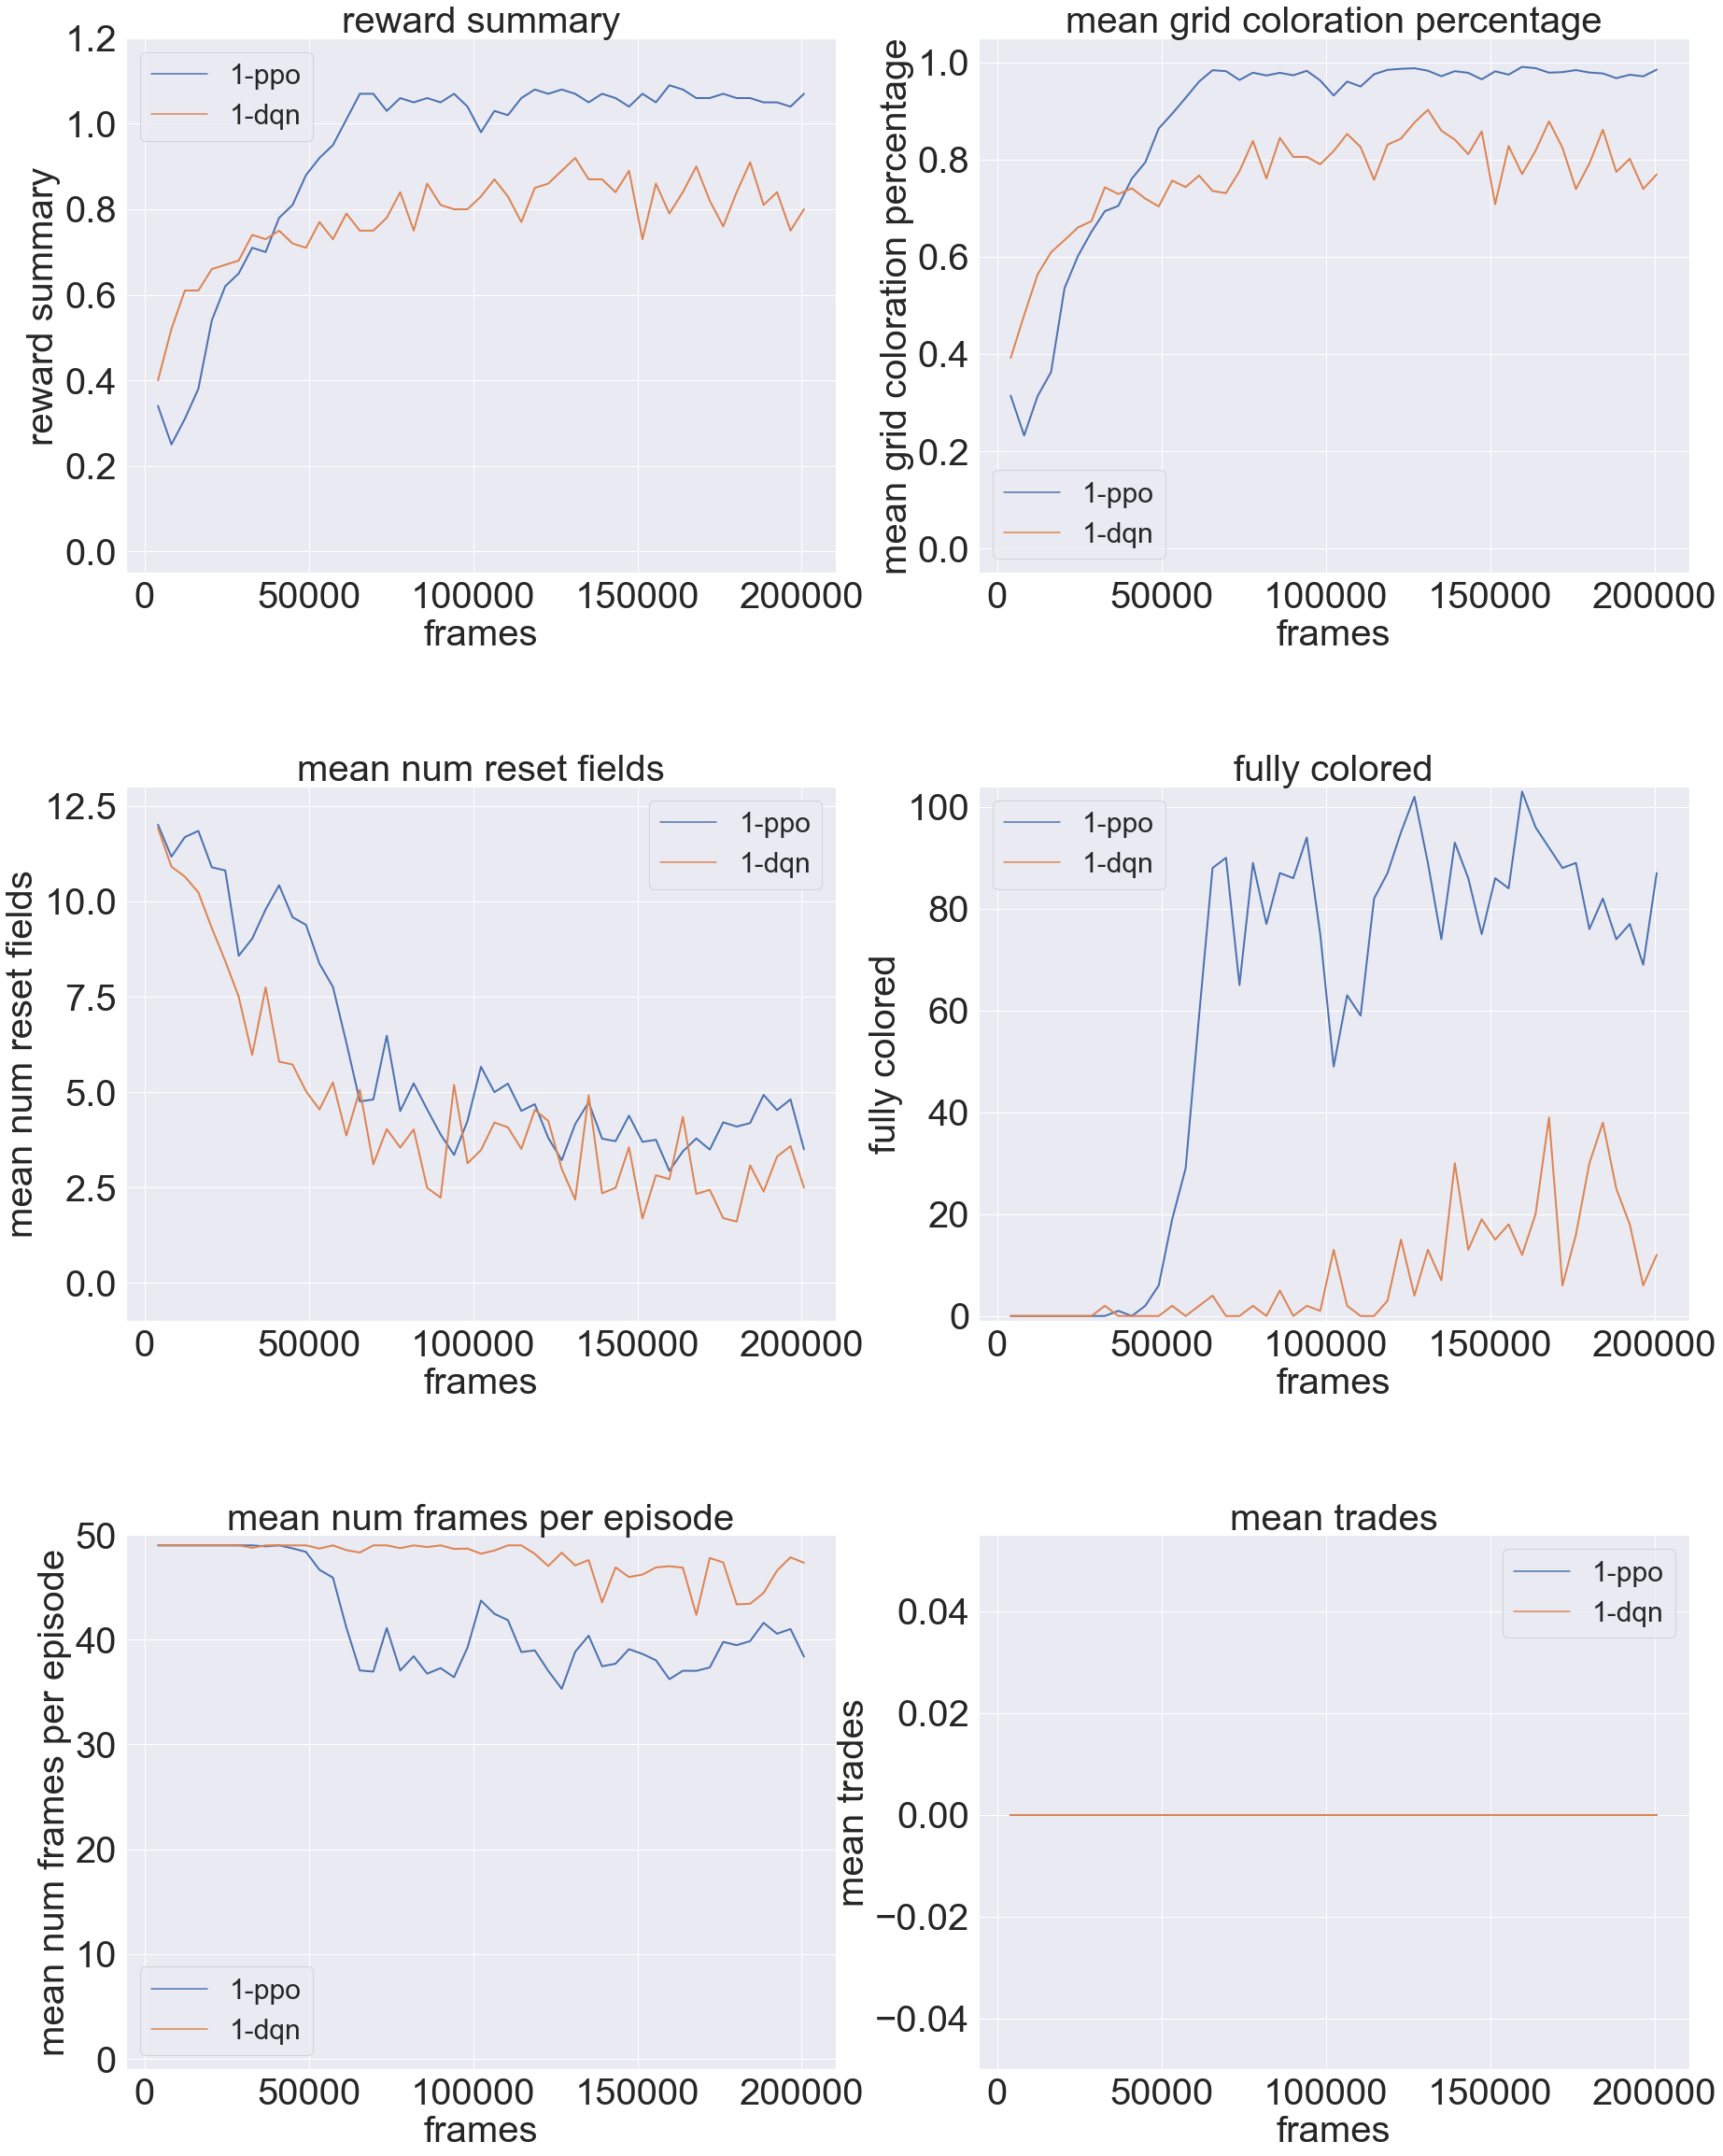
\includegraphics[width=1\textwidth]{AX-hard-1.png}\\
    \caption[PPO and DQN Training Details with One Agent in a 7x7 Environment]{Details of the training  in a 7x7 Environment with one agent using PPO and DQN}\label{fig:ax-hard-1}
\end{figure}
\vfill
\clearpage


\newpage
\vfill
\begin{figure}
    \centering
    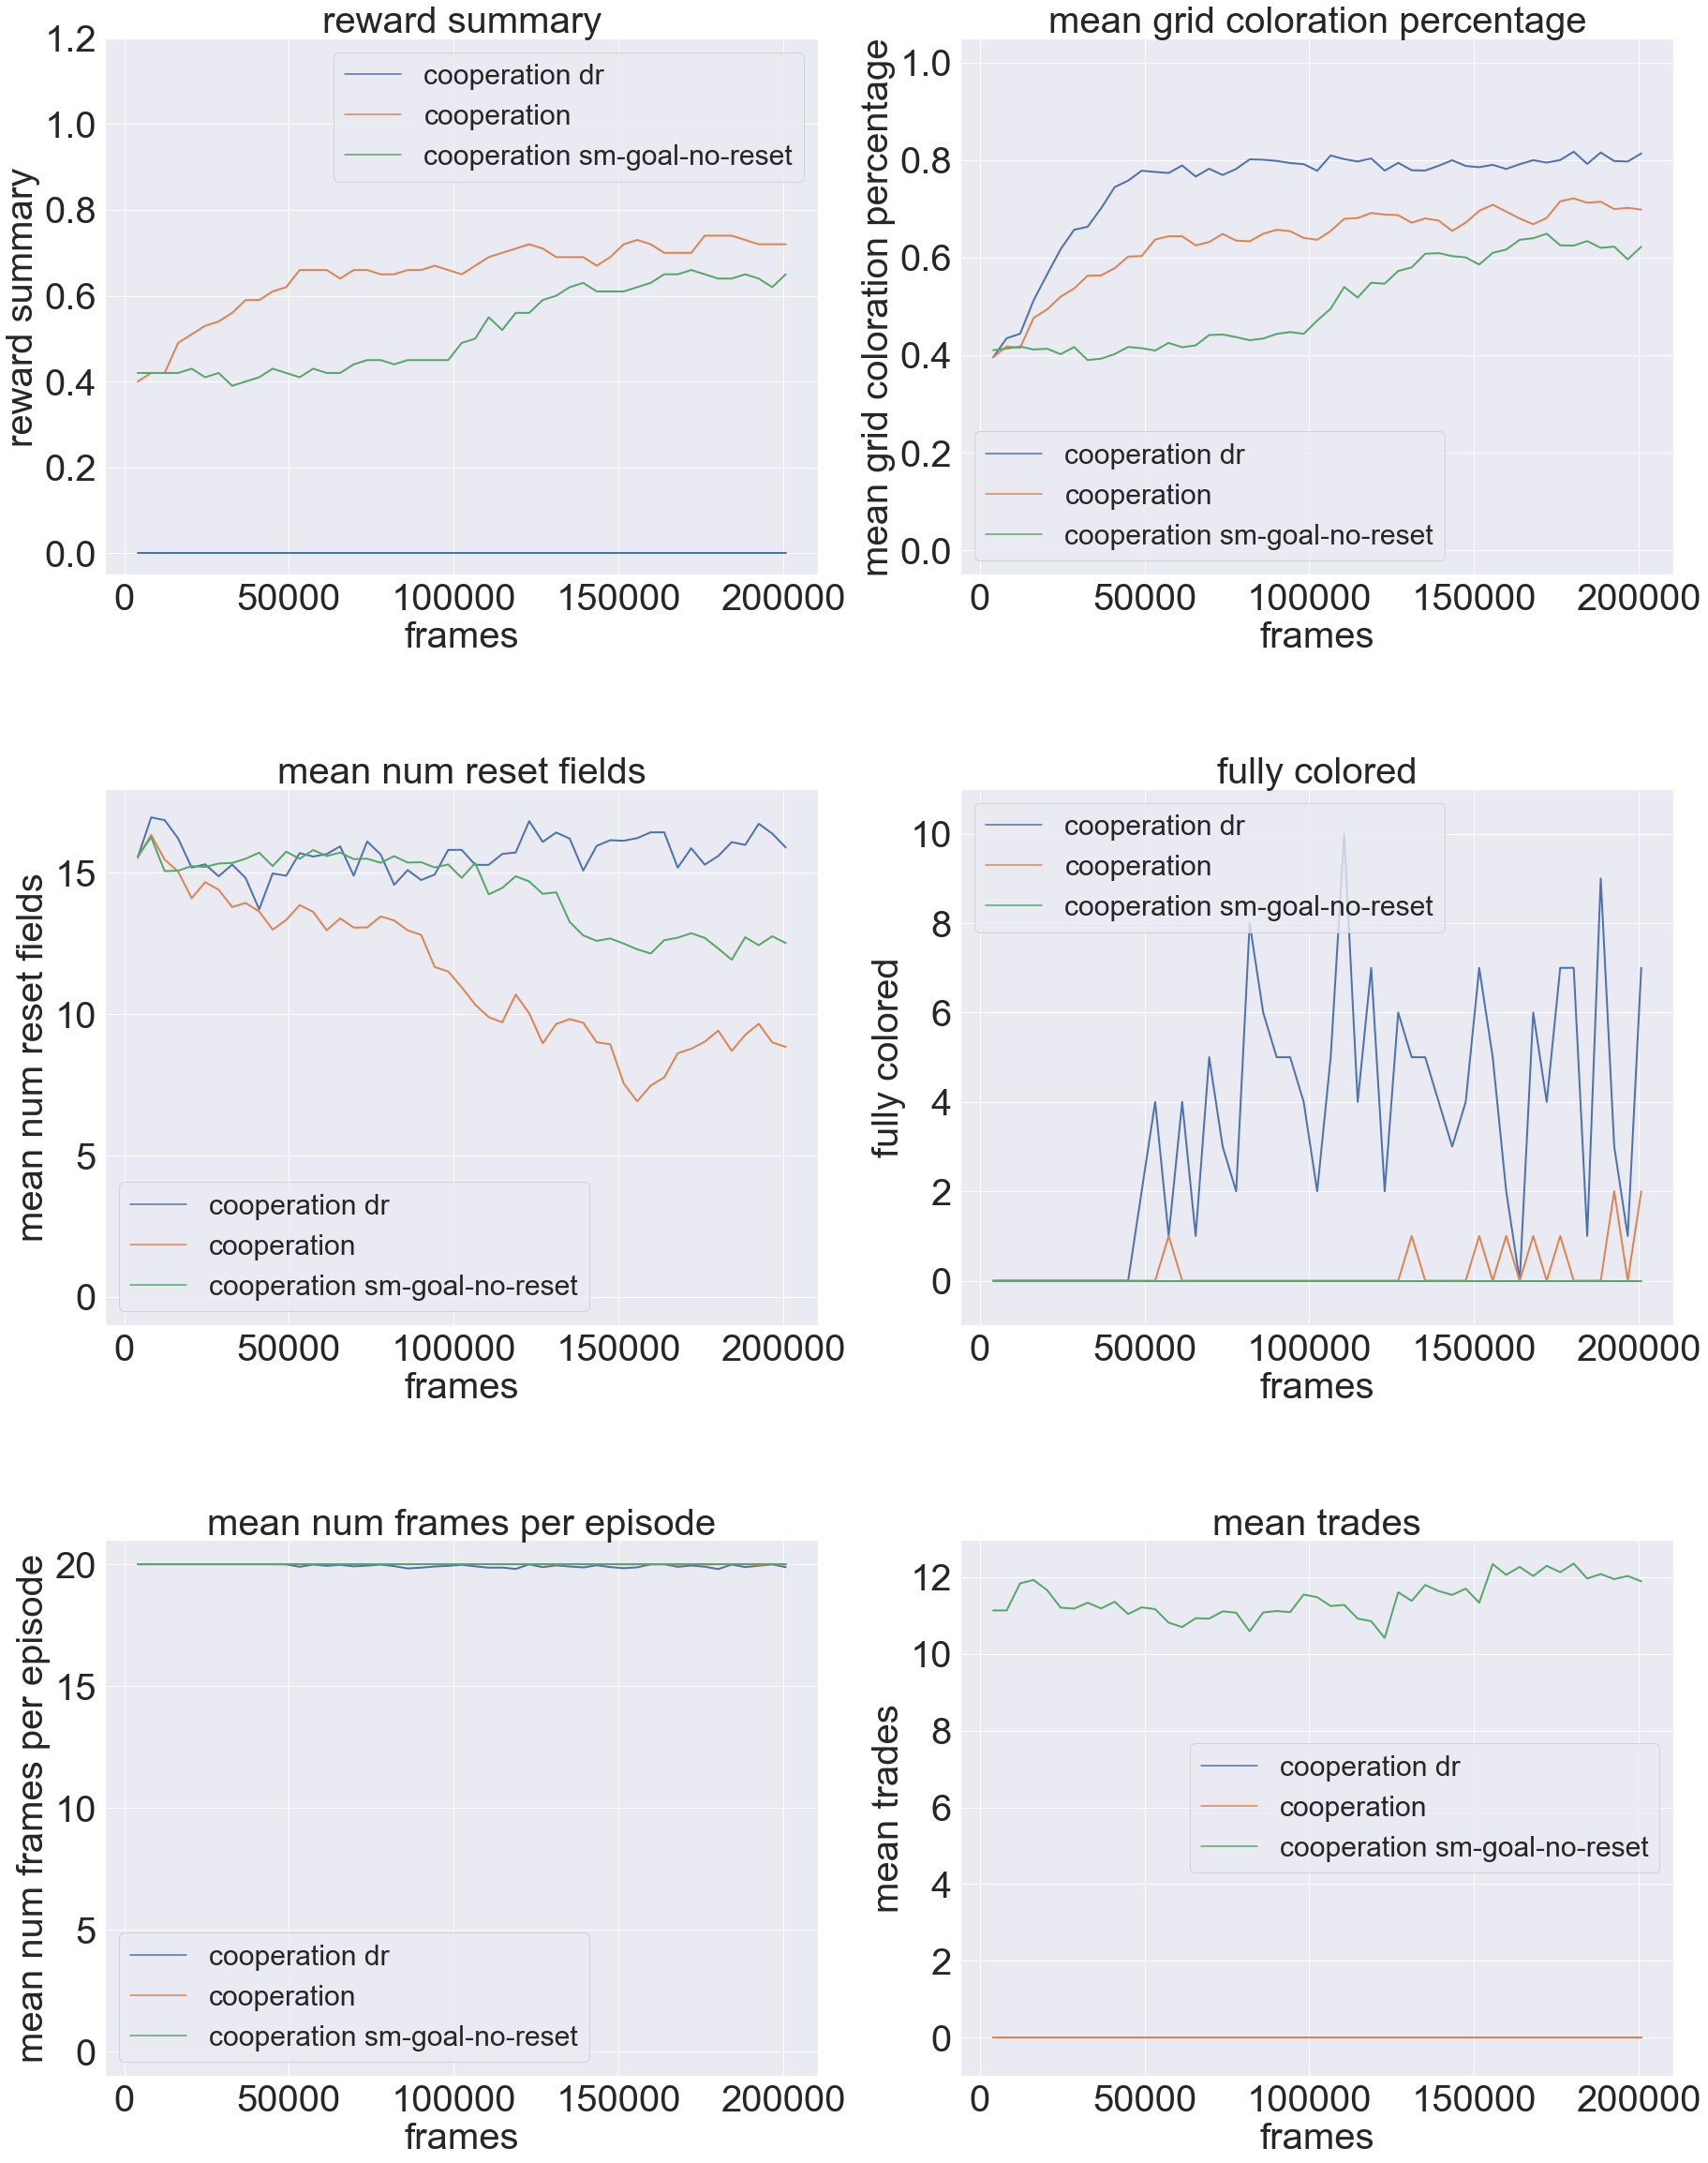
\includegraphics[width=1\textwidth]{AX-hard-3-ppo-coop.png}\\
    \caption[Training Details of Top PPO Cooperation Executions in a 7x7 Environment]{Top cooperation score details of three PPO agents in a 7x7 Environment}\label{fig:ax-hard-2-ppo-coop}
\end{figure}
\vfill
\clearpage


\newpage
\vfill
\begin{figure}
    \centering
    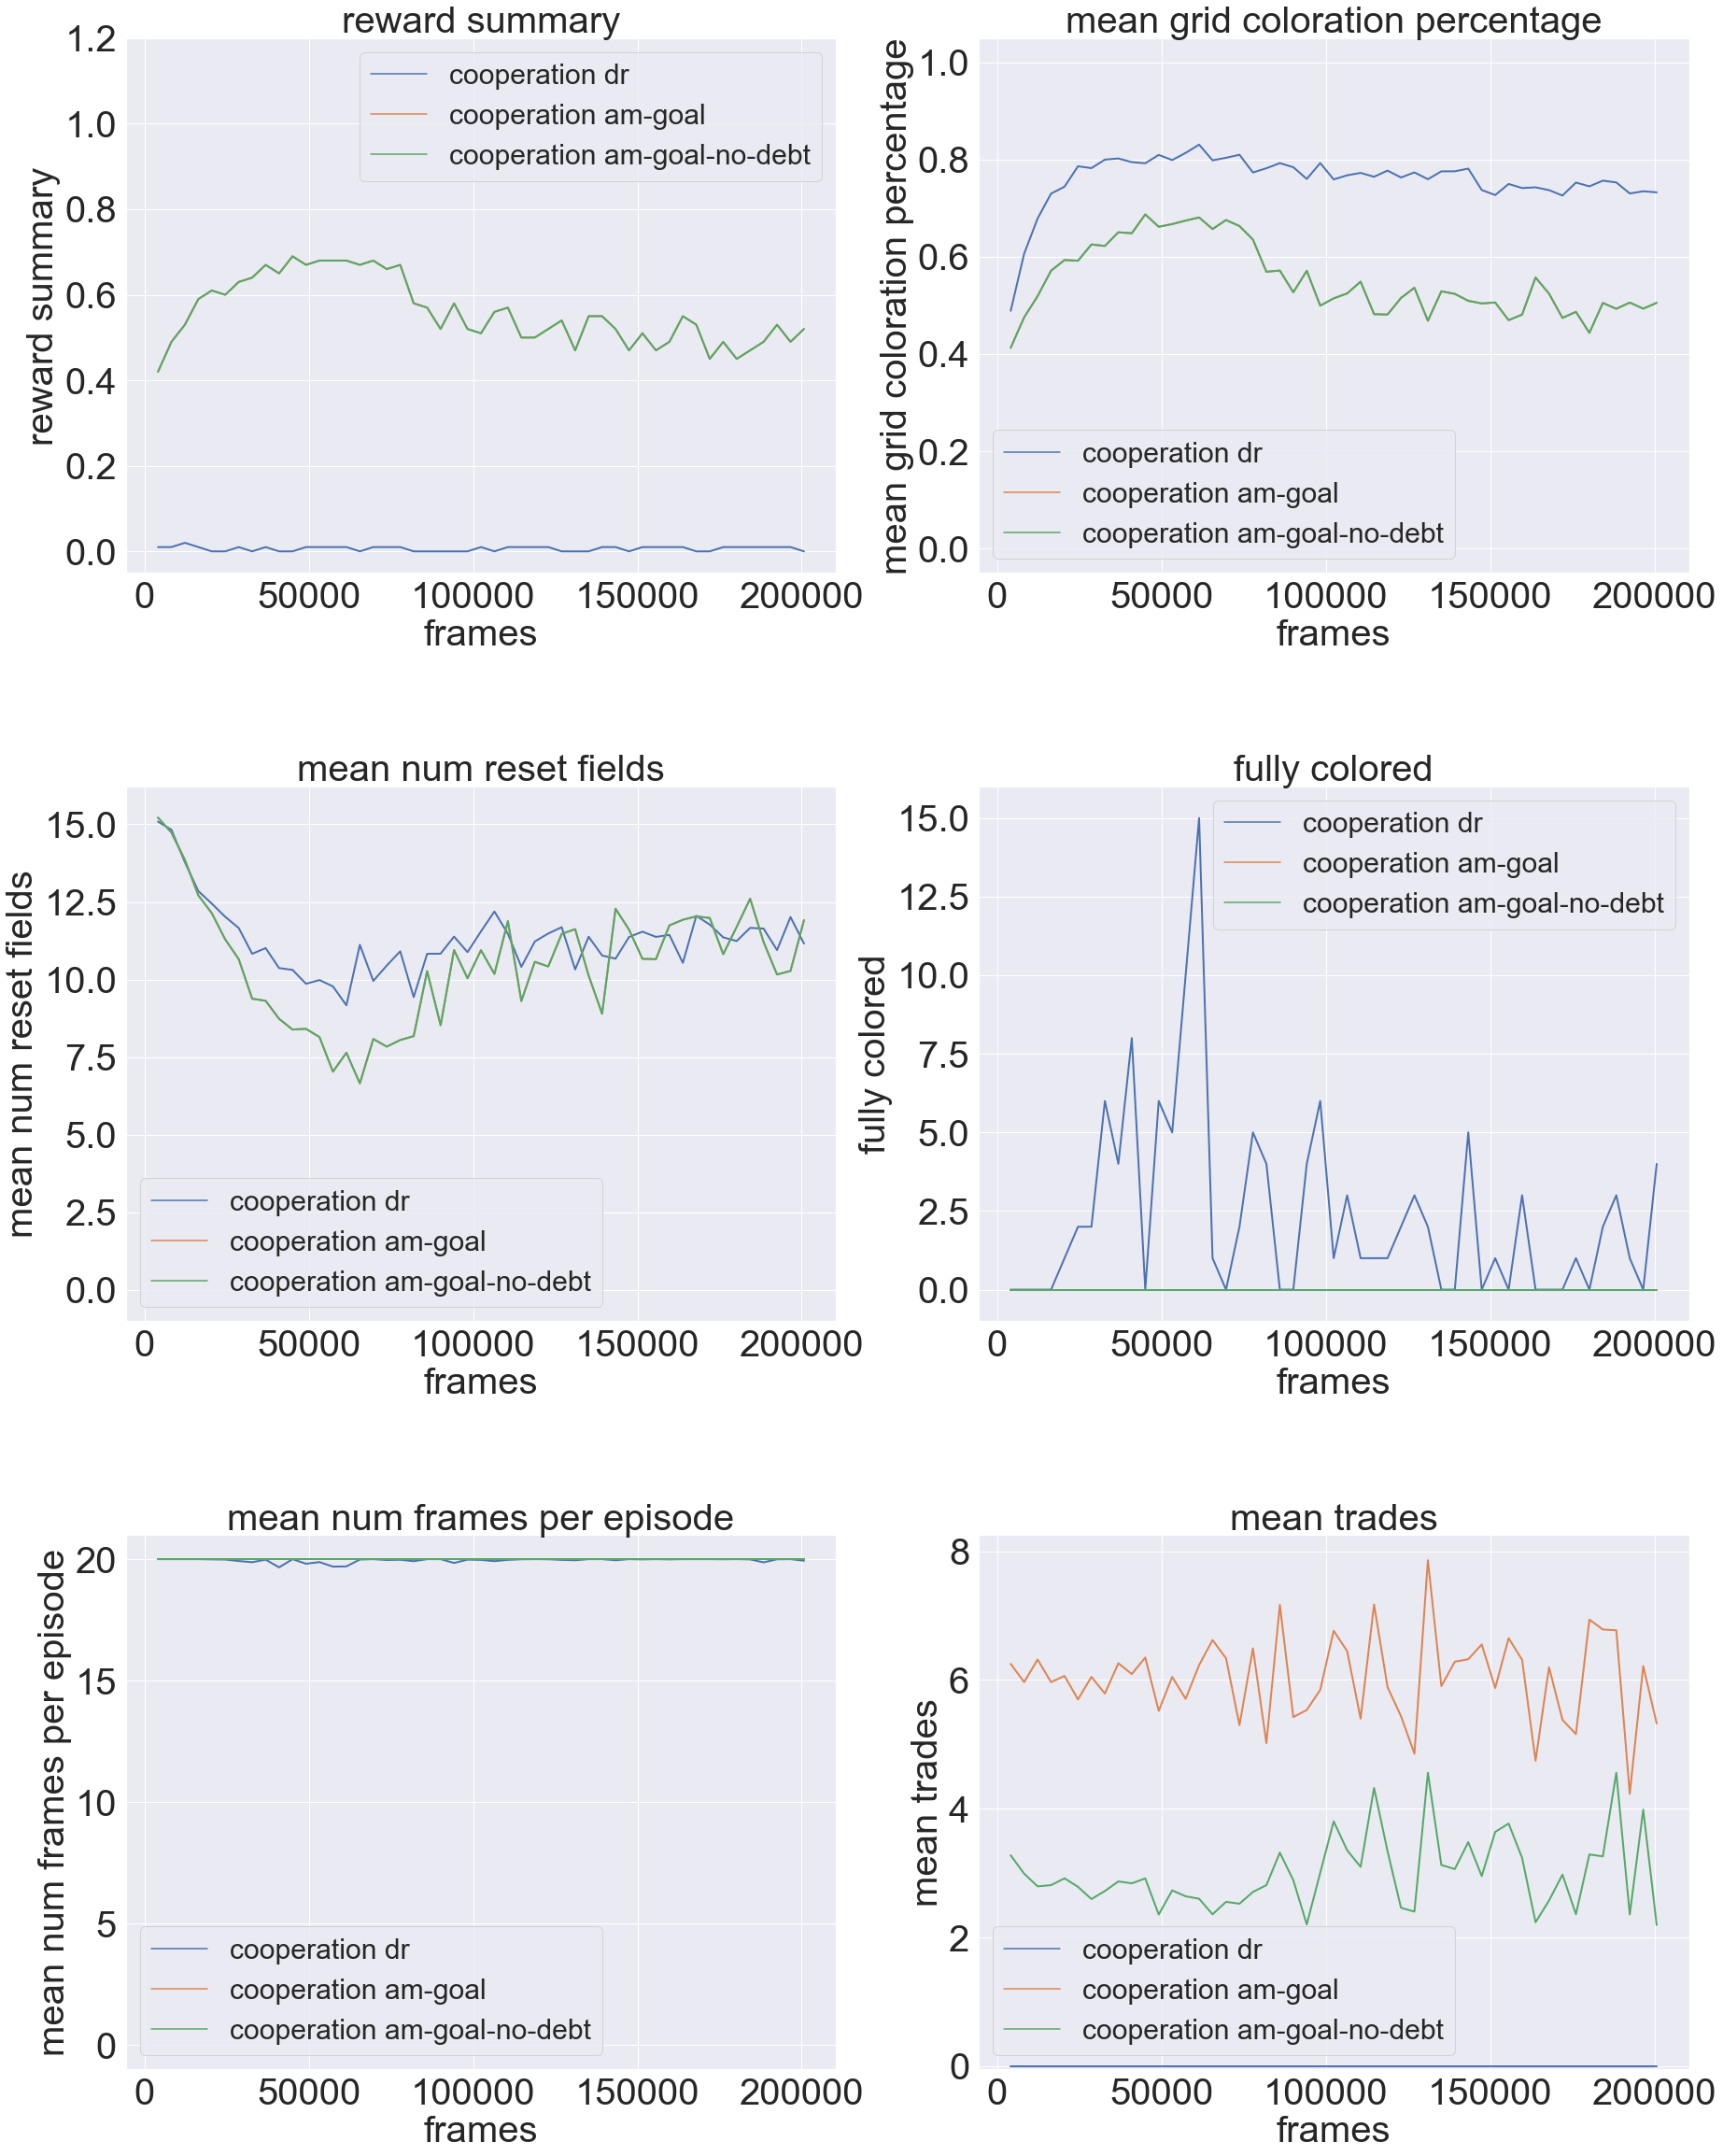
\includegraphics[width=1\textwidth]{AX-hard-3-dqn-coop.png}\\
    \caption[Training Details of Top DQN Cooperation Executions in a 7x7 Environment]{Top cooperation score details of three DQN agents in a 7x7 Environment}\label{fig:ax-hard-2-dqn-coop}
\end{figure}
\vfill
\clearpage


\newpage
\vfill
\begin{figure}
    \centering
    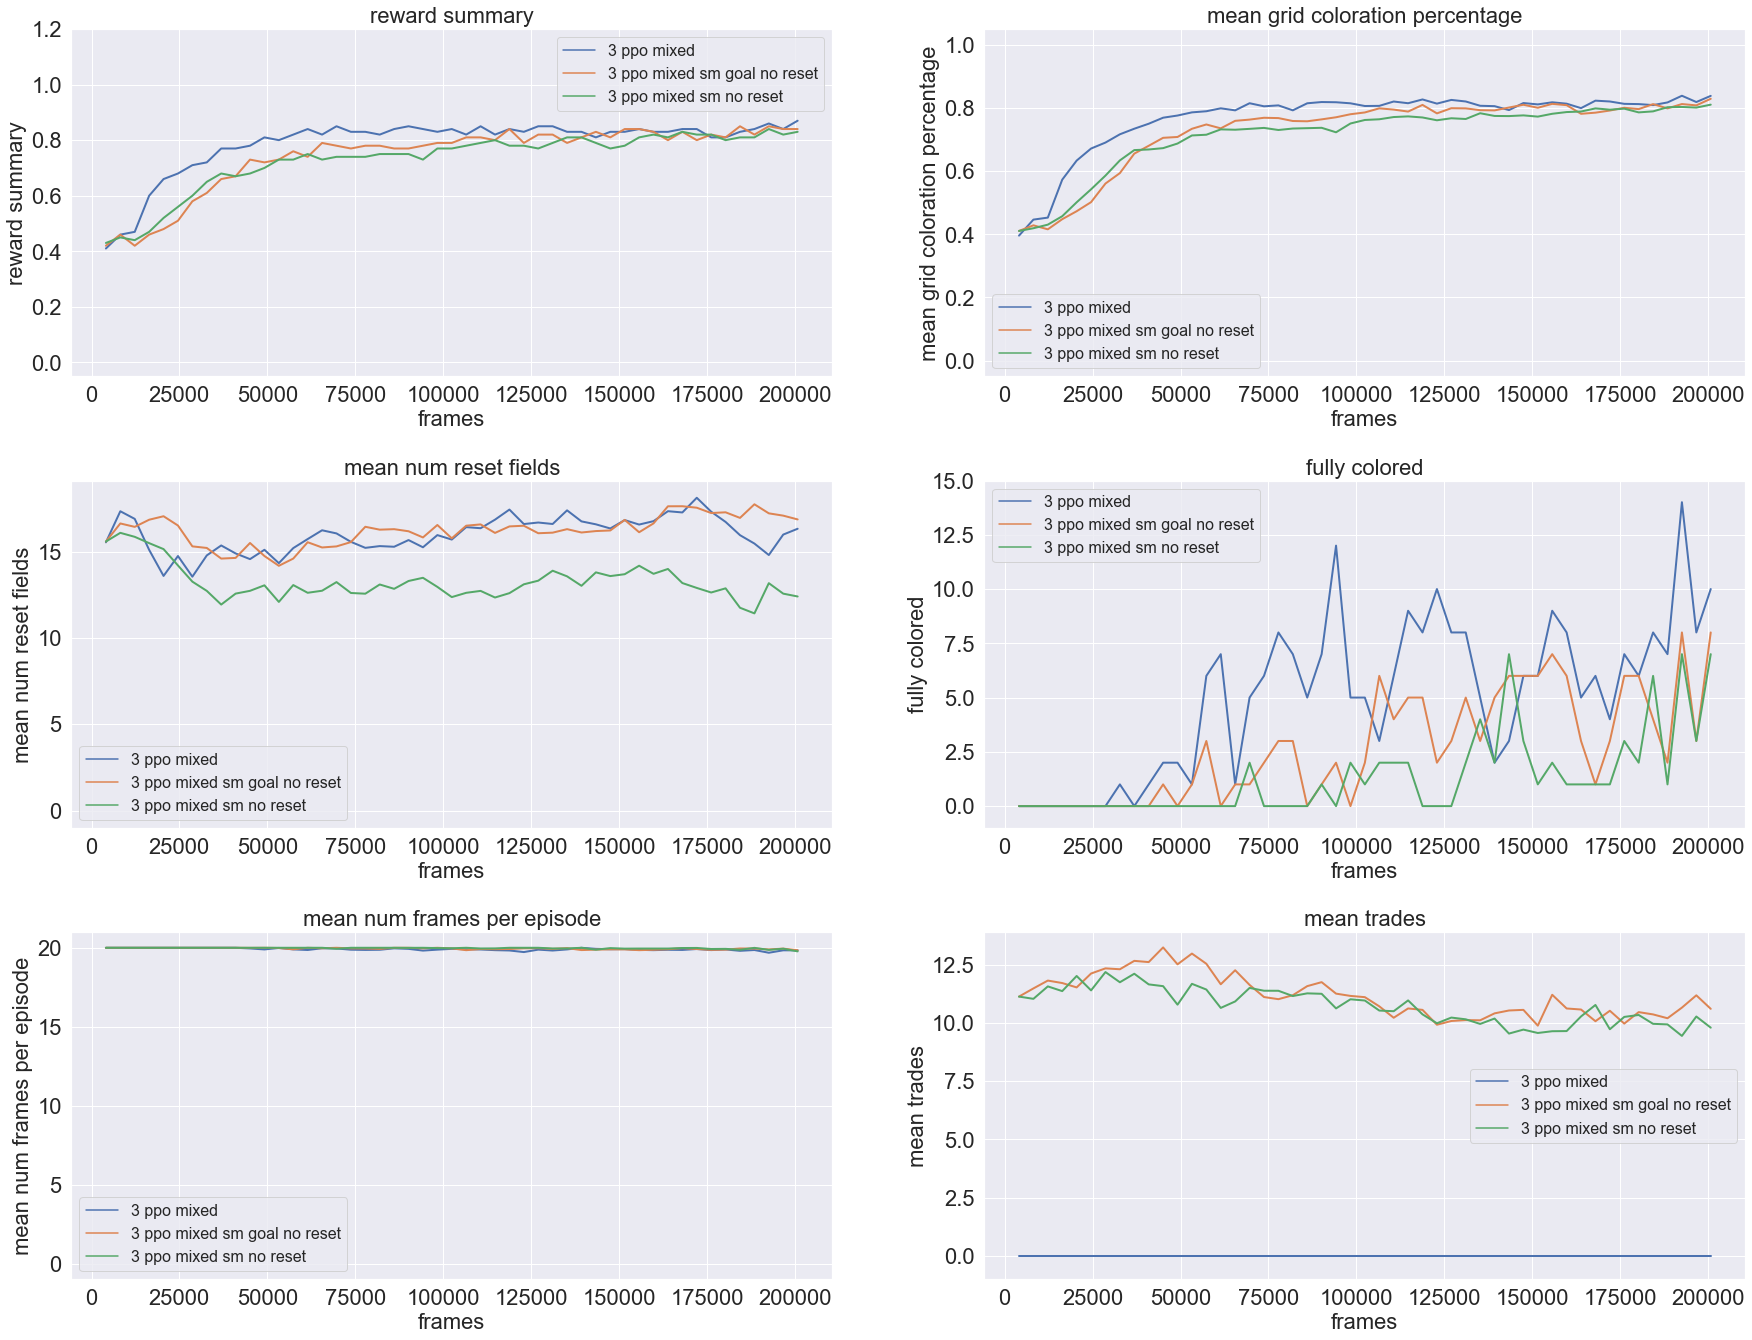
\includegraphics[width=1\textwidth]{AX-hard-3-ppo-mixed.png}\\
    \caption[Training Details of Top PPO Mixed-Motive Executions in a 7x7 Environment]{Top mixed-motive score details of three PPO agents in a 7x7 Environment}\label{fig:ax-hard-2-ppo-mixed}
\end{figure}
\vfill
\clearpage


\newpage
\vfill
\begin{figure}
    \centering
    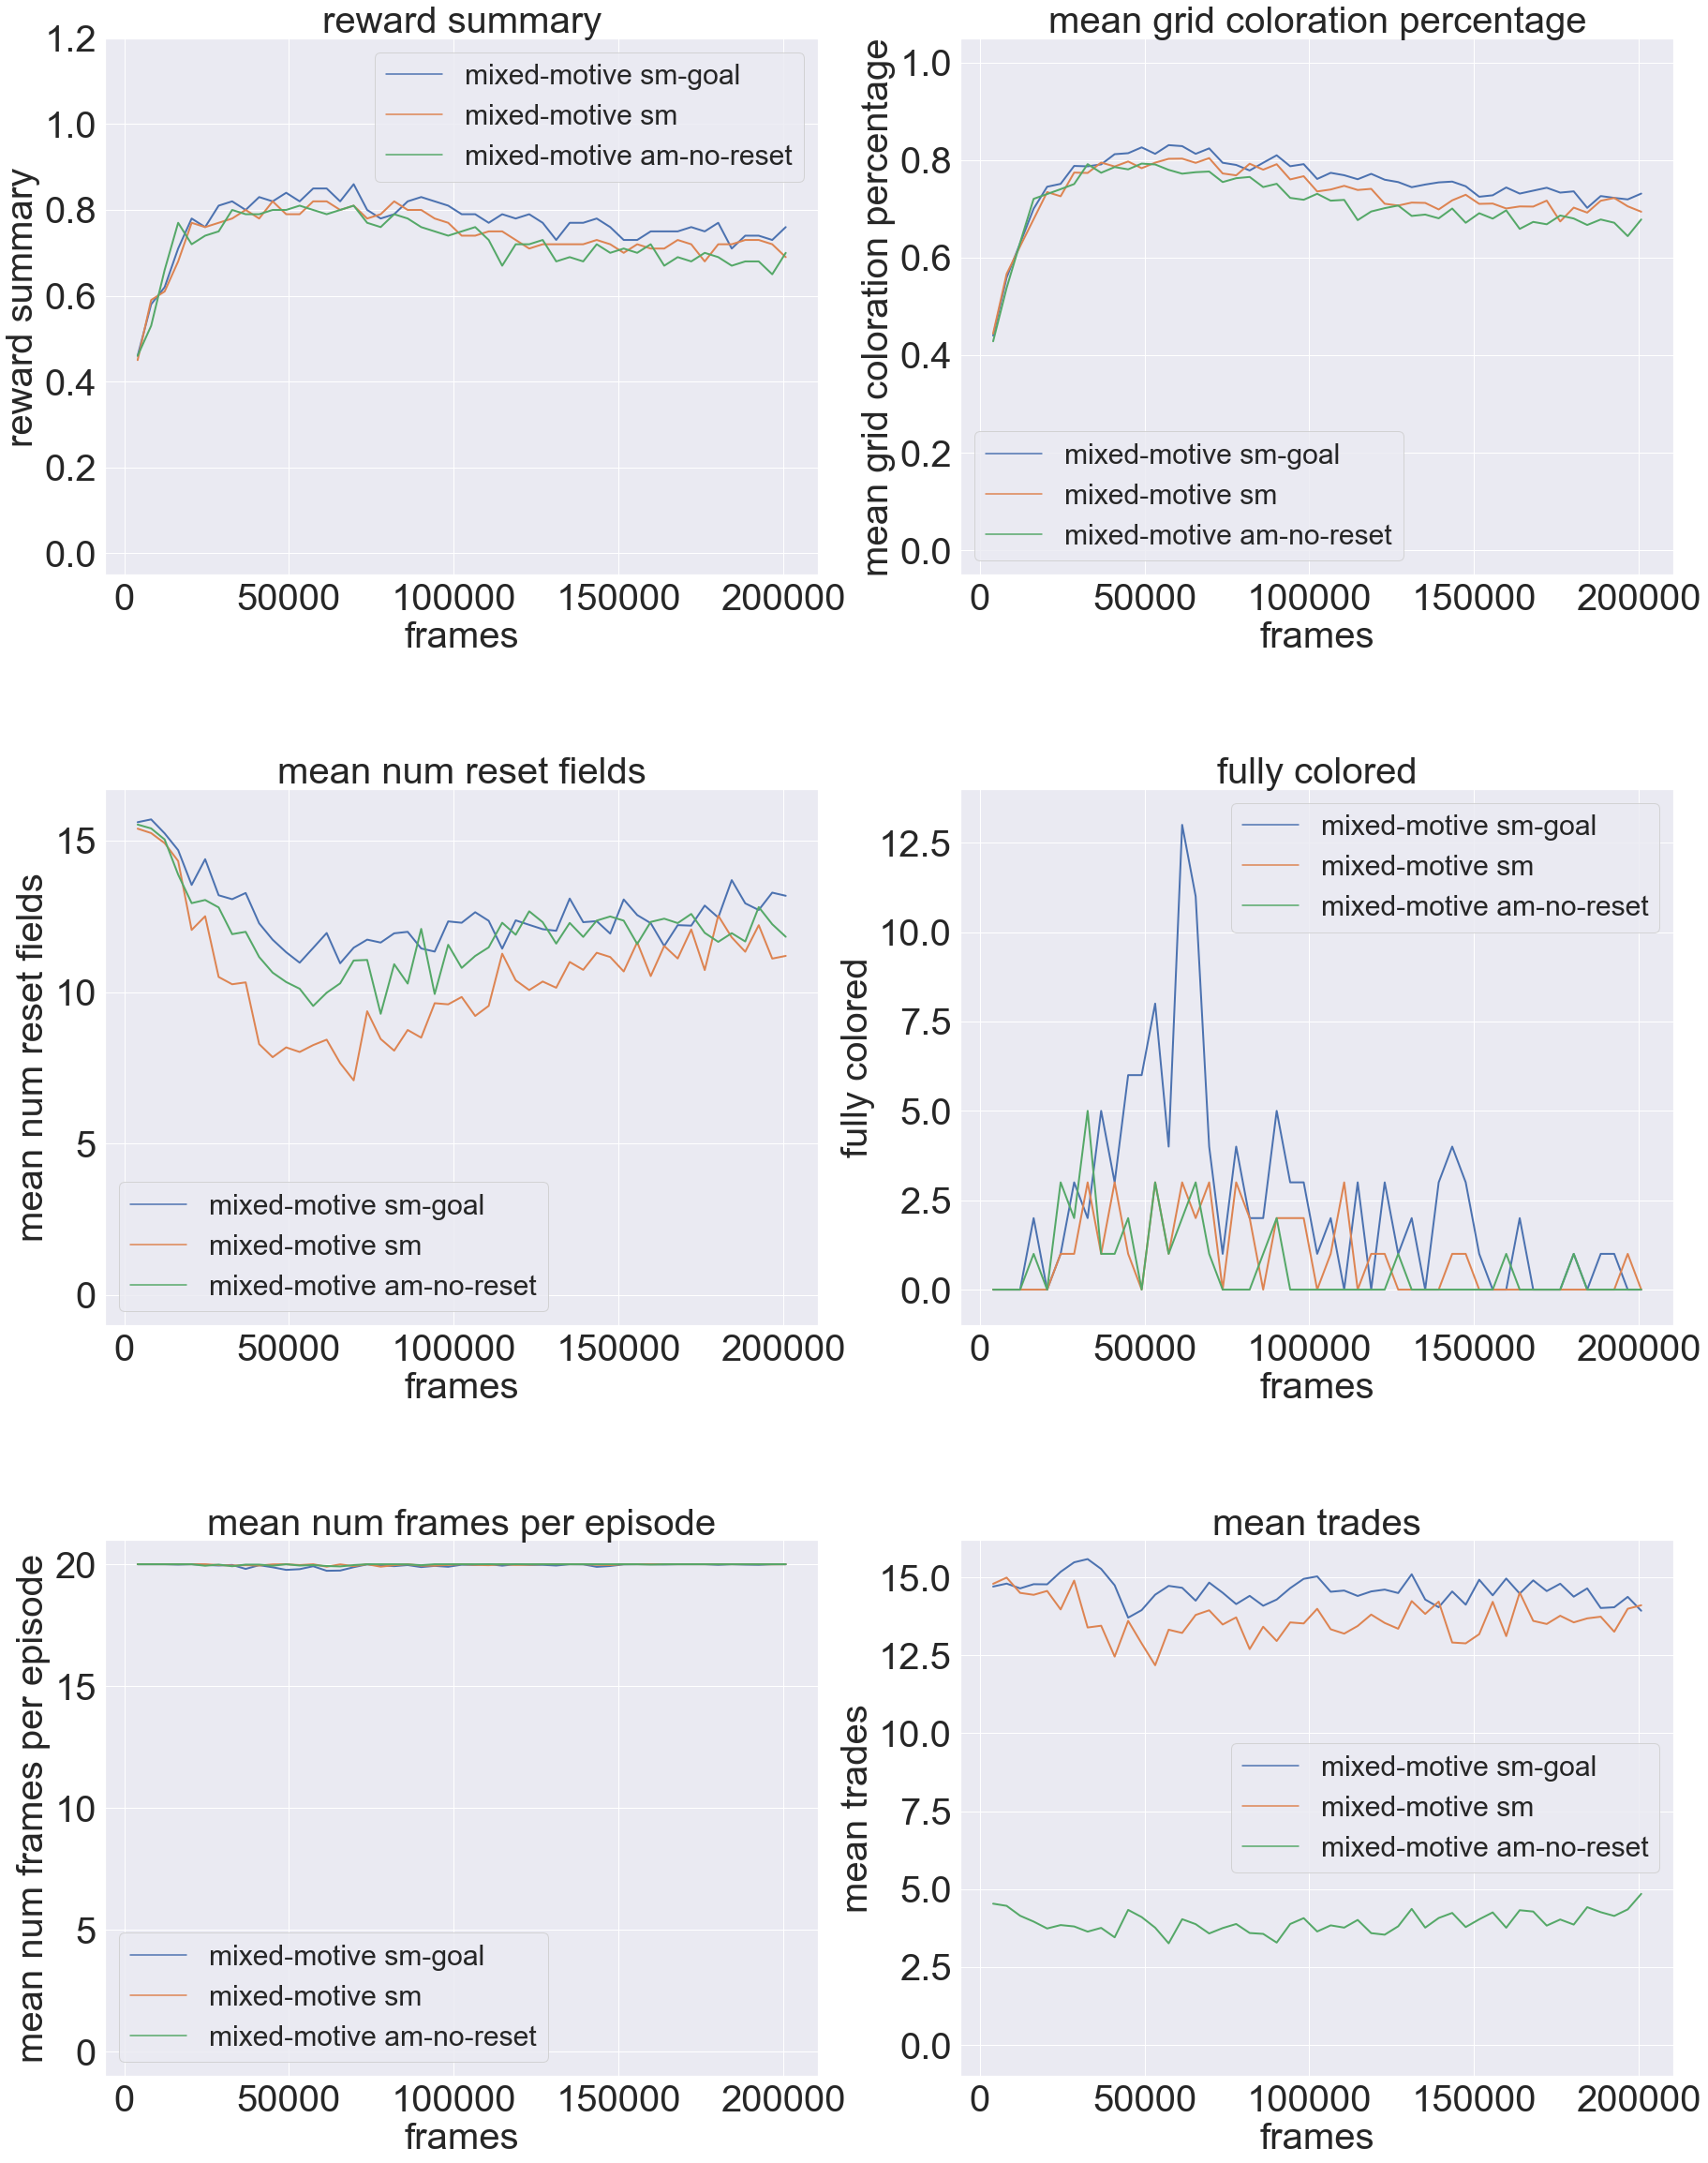
\includegraphics[width=1\textwidth]{AX-hard-3-dqn-mixed.png}\\
    \caption[Training Details of Top DQN Mixed-Motive Executions in a 7x7 Environment]{Top mixed-motive score details of three DQN agents in a 7x7 Environment}\label{fig:ax-hard-2-dqn-mixed}
\end{figure}
\vfill
\clearpage


\newpage
\vfill
\begin{figure}
    \centering
    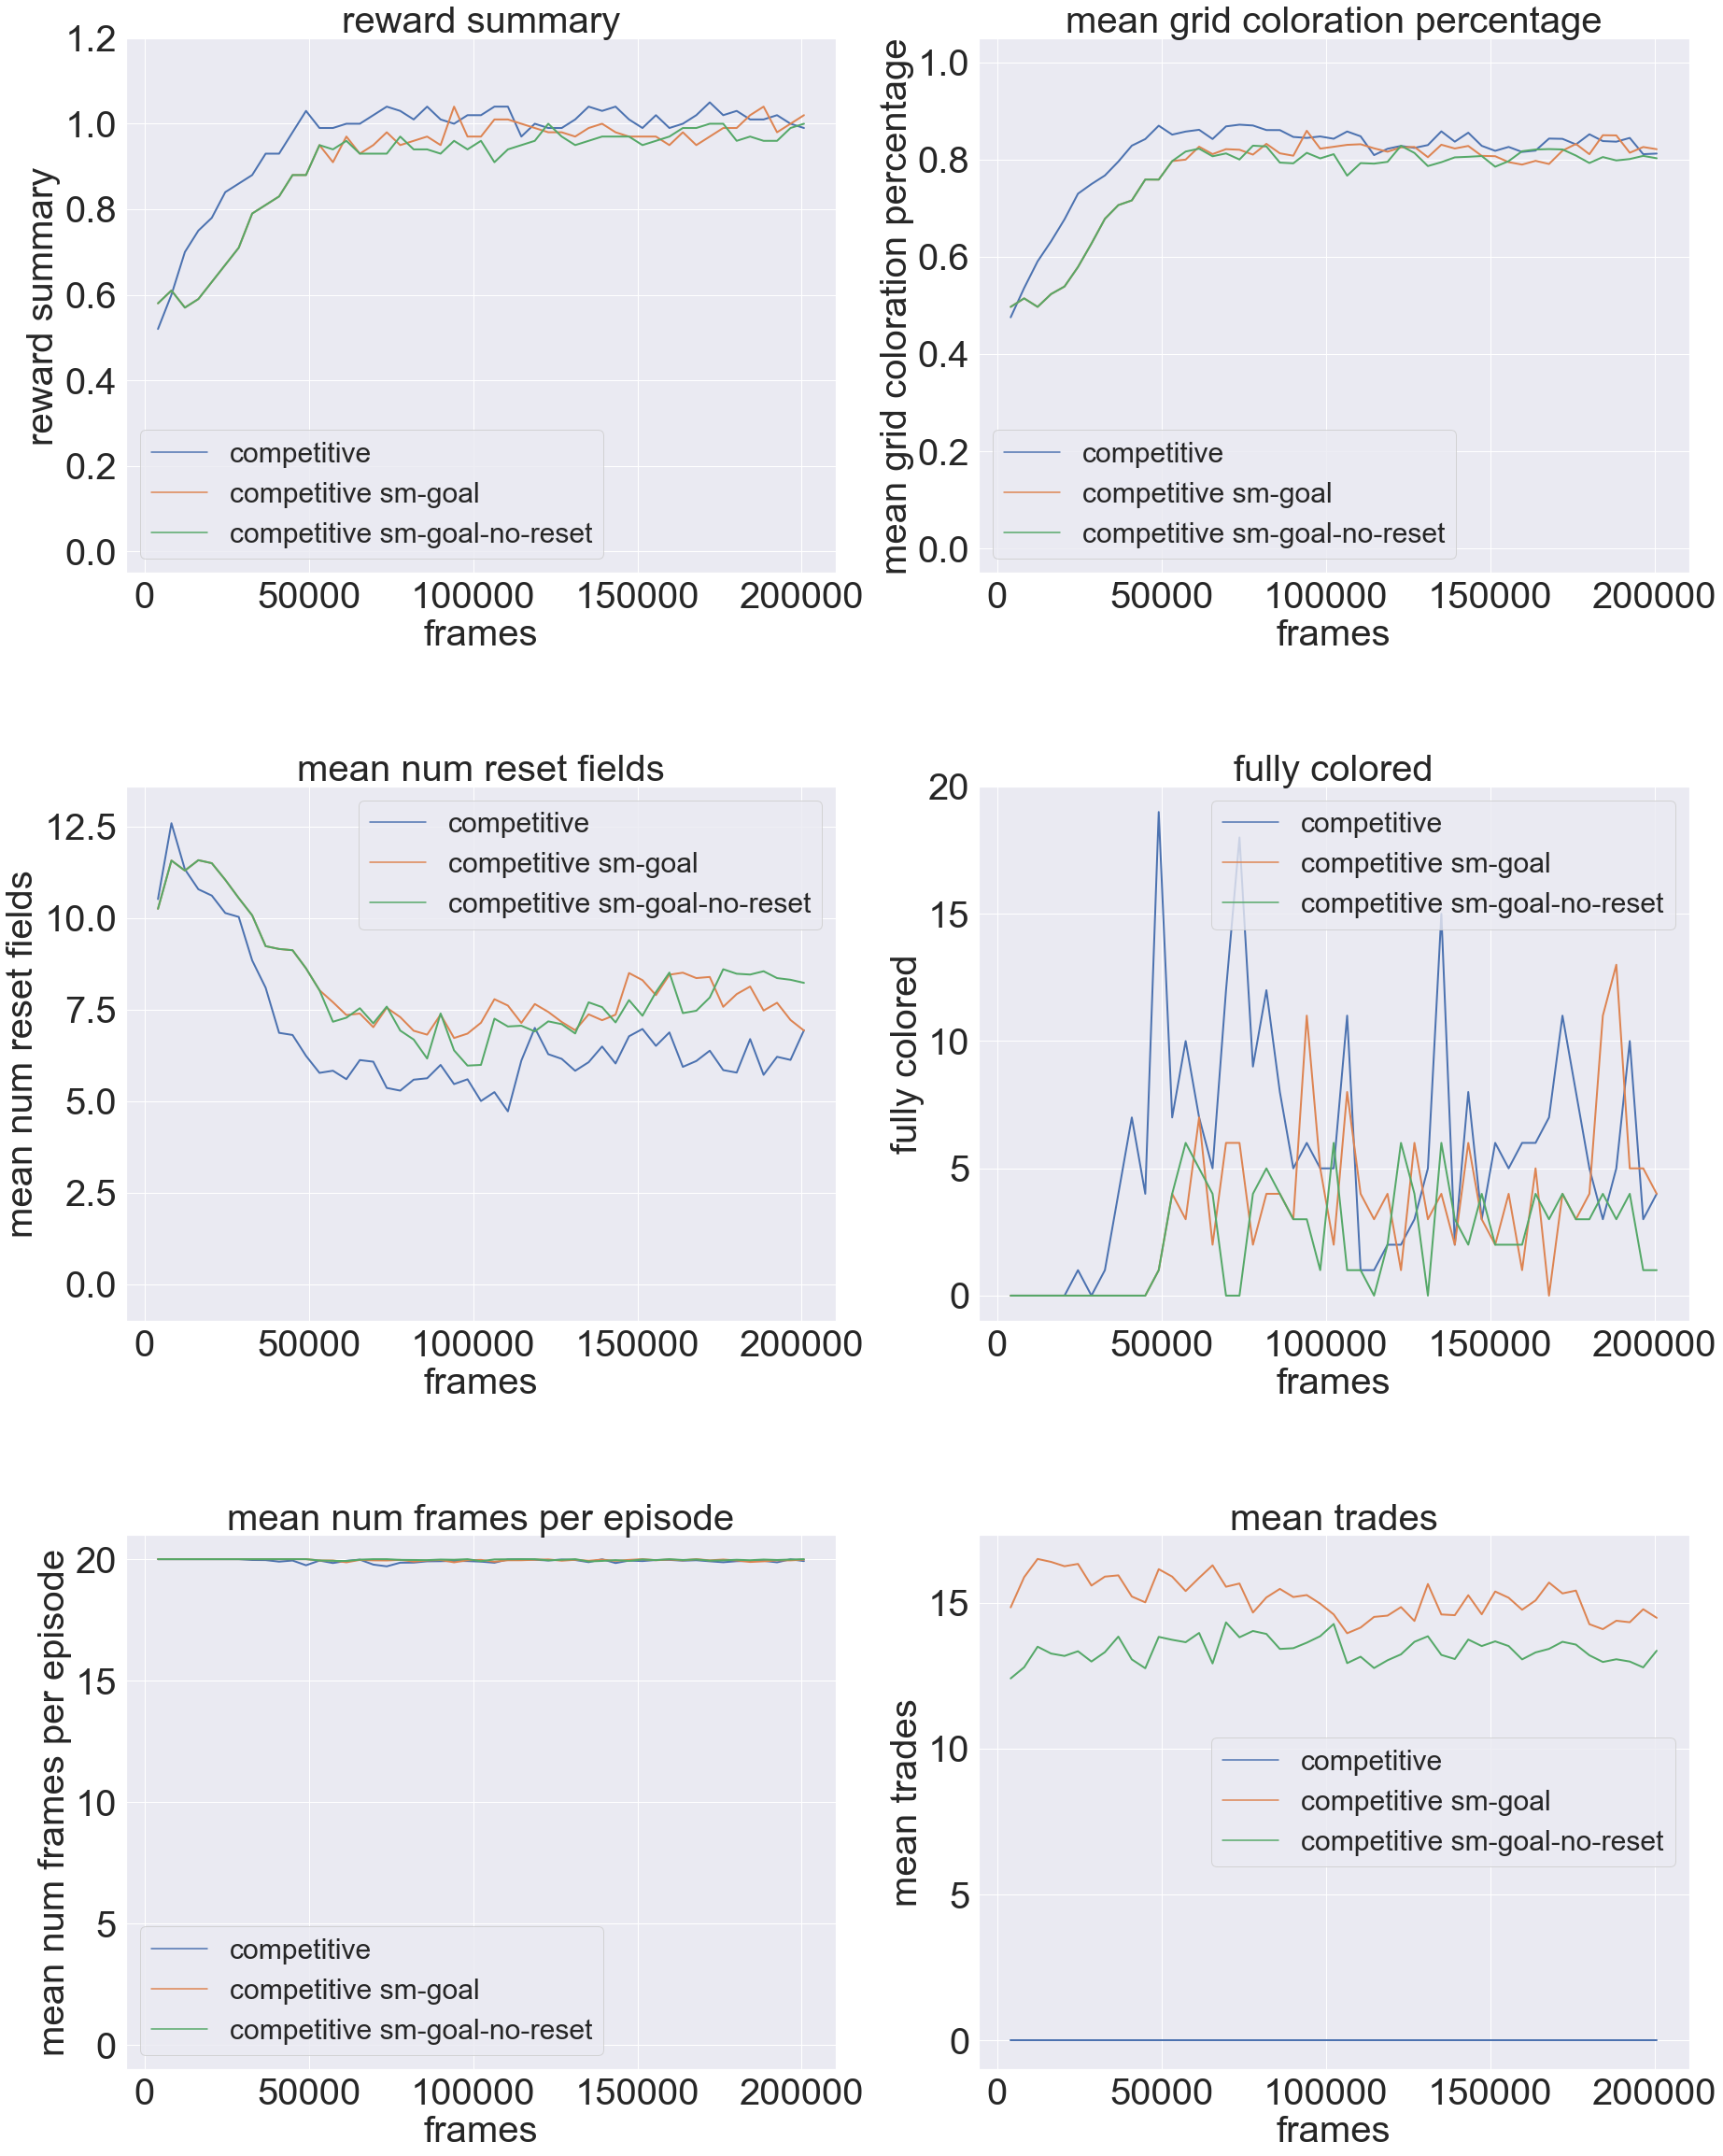
\includegraphics[width=1\textwidth]{AX-hard-3-ppo-comp.png}\\
    \caption[Training Details of Top PPO Competitive Executions in a 7x7 Environment]{Top competitive score details of three PPO agents in a 7x7 Environment}\label{fig:ax-hard-2-ppo-comp}
\end{figure}
\vfill
\clearpage


\newpage
\vfill
\begin{figure}
    \centering
    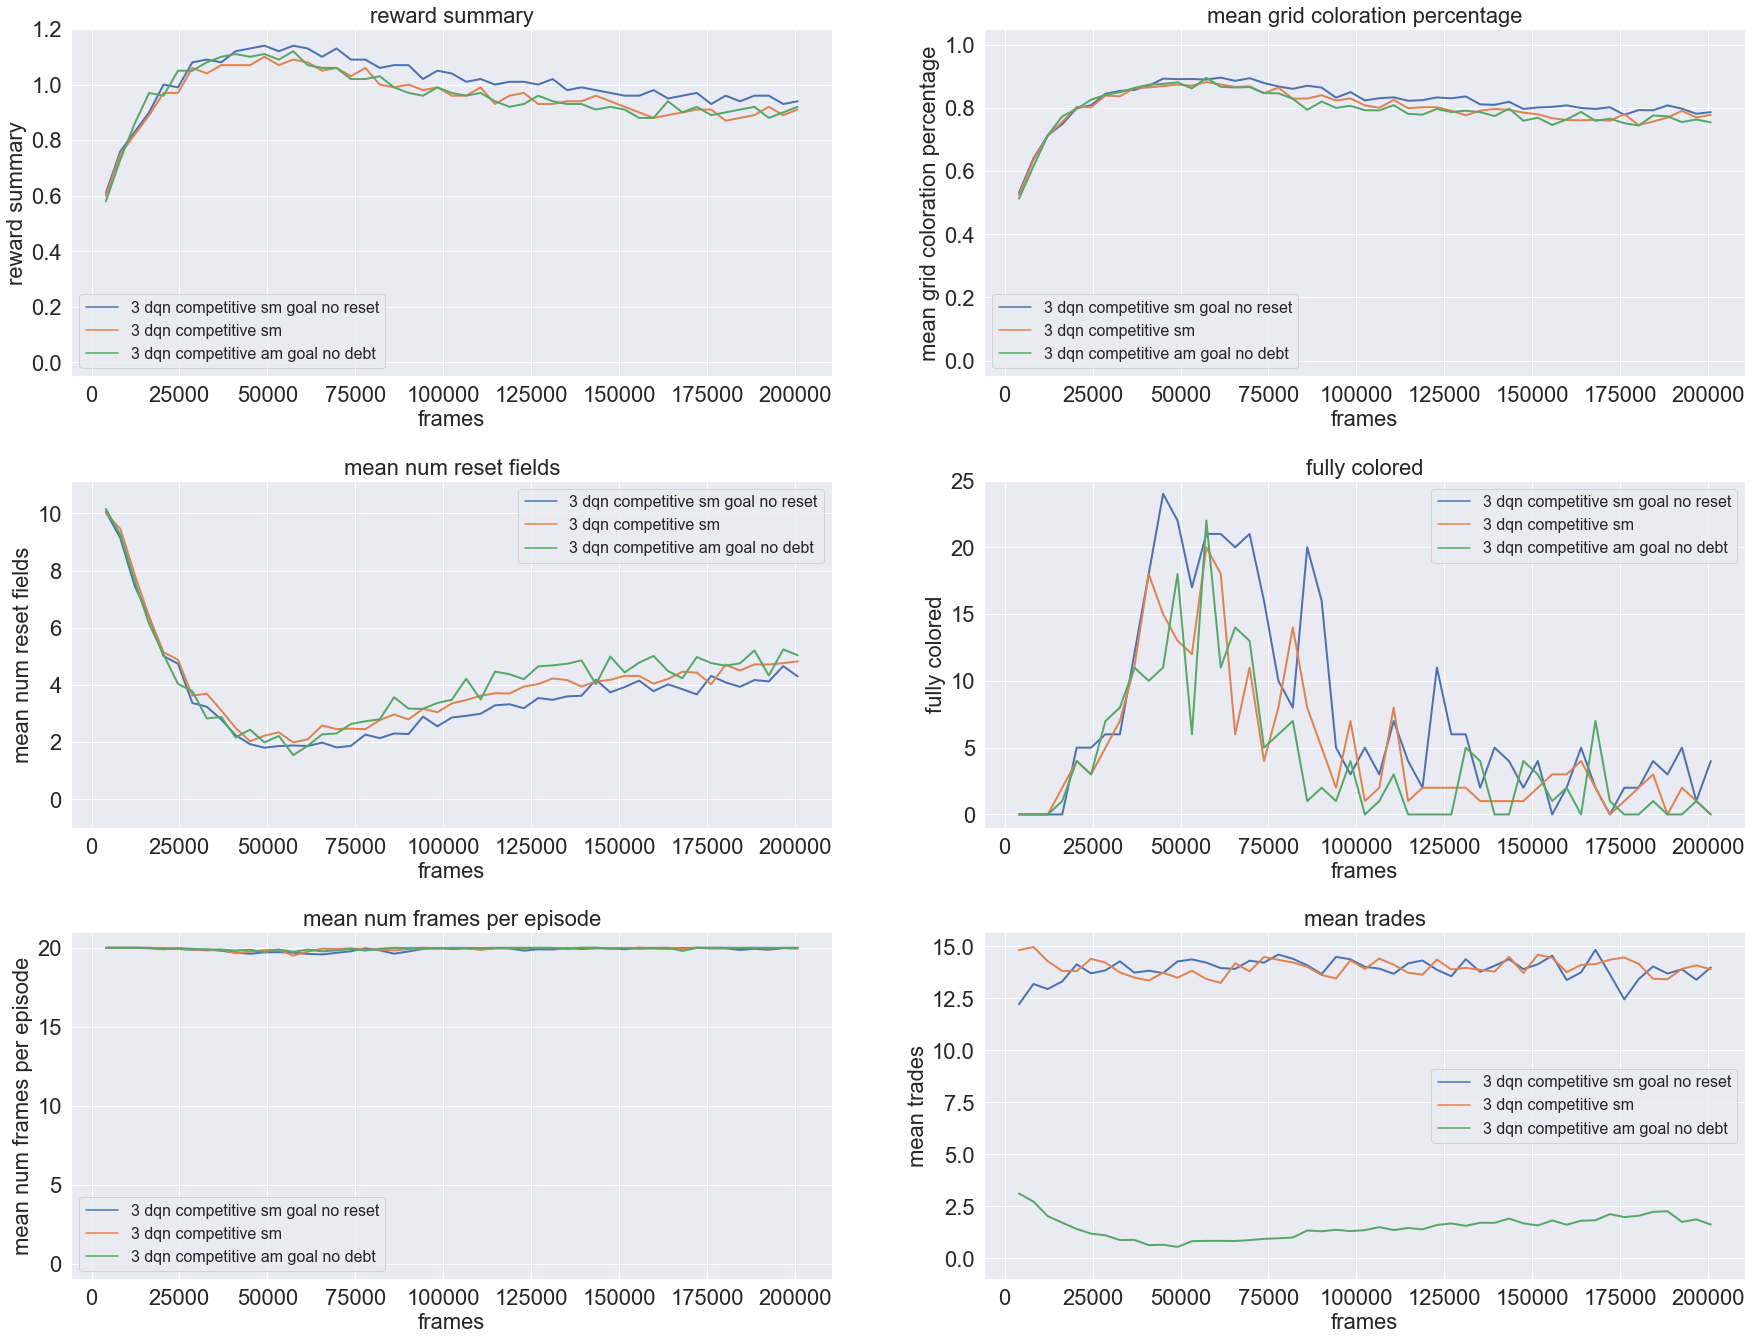
\includegraphics[width=1\textwidth]{AX-hard-3-dqn-comp.png}\\
    \caption[Training Details of Top DQN Competitive Executions in a 7x7 Environment]{Top competitive score details of three DQN agents in a 7x7 Environment}\label{fig:ax-hard-2-dqn-comp}
\end{figure}
\vfill
\clearpage


\subsection{Rooms Environment}
An example to run a training process in a nine by nine room divided environment is shown below.

\begin{lstlisting}[float=htp,language=bash, escapeinside={//@}{@//},xleftmargin=3ex,xrightmargin=1ex]
$ python -m scripts.train 
    --algo ppo 
    --agents 3 
    --model ppo-rooms
    --env FourRooms-Grid-v0 
    --grid-size 9 
    --max-steps 30 
    --frames-per-proc 256 
    --frames 200000 
\end{lstlisting}

\newpage
\vfill
\begin{figure}
    \centering
    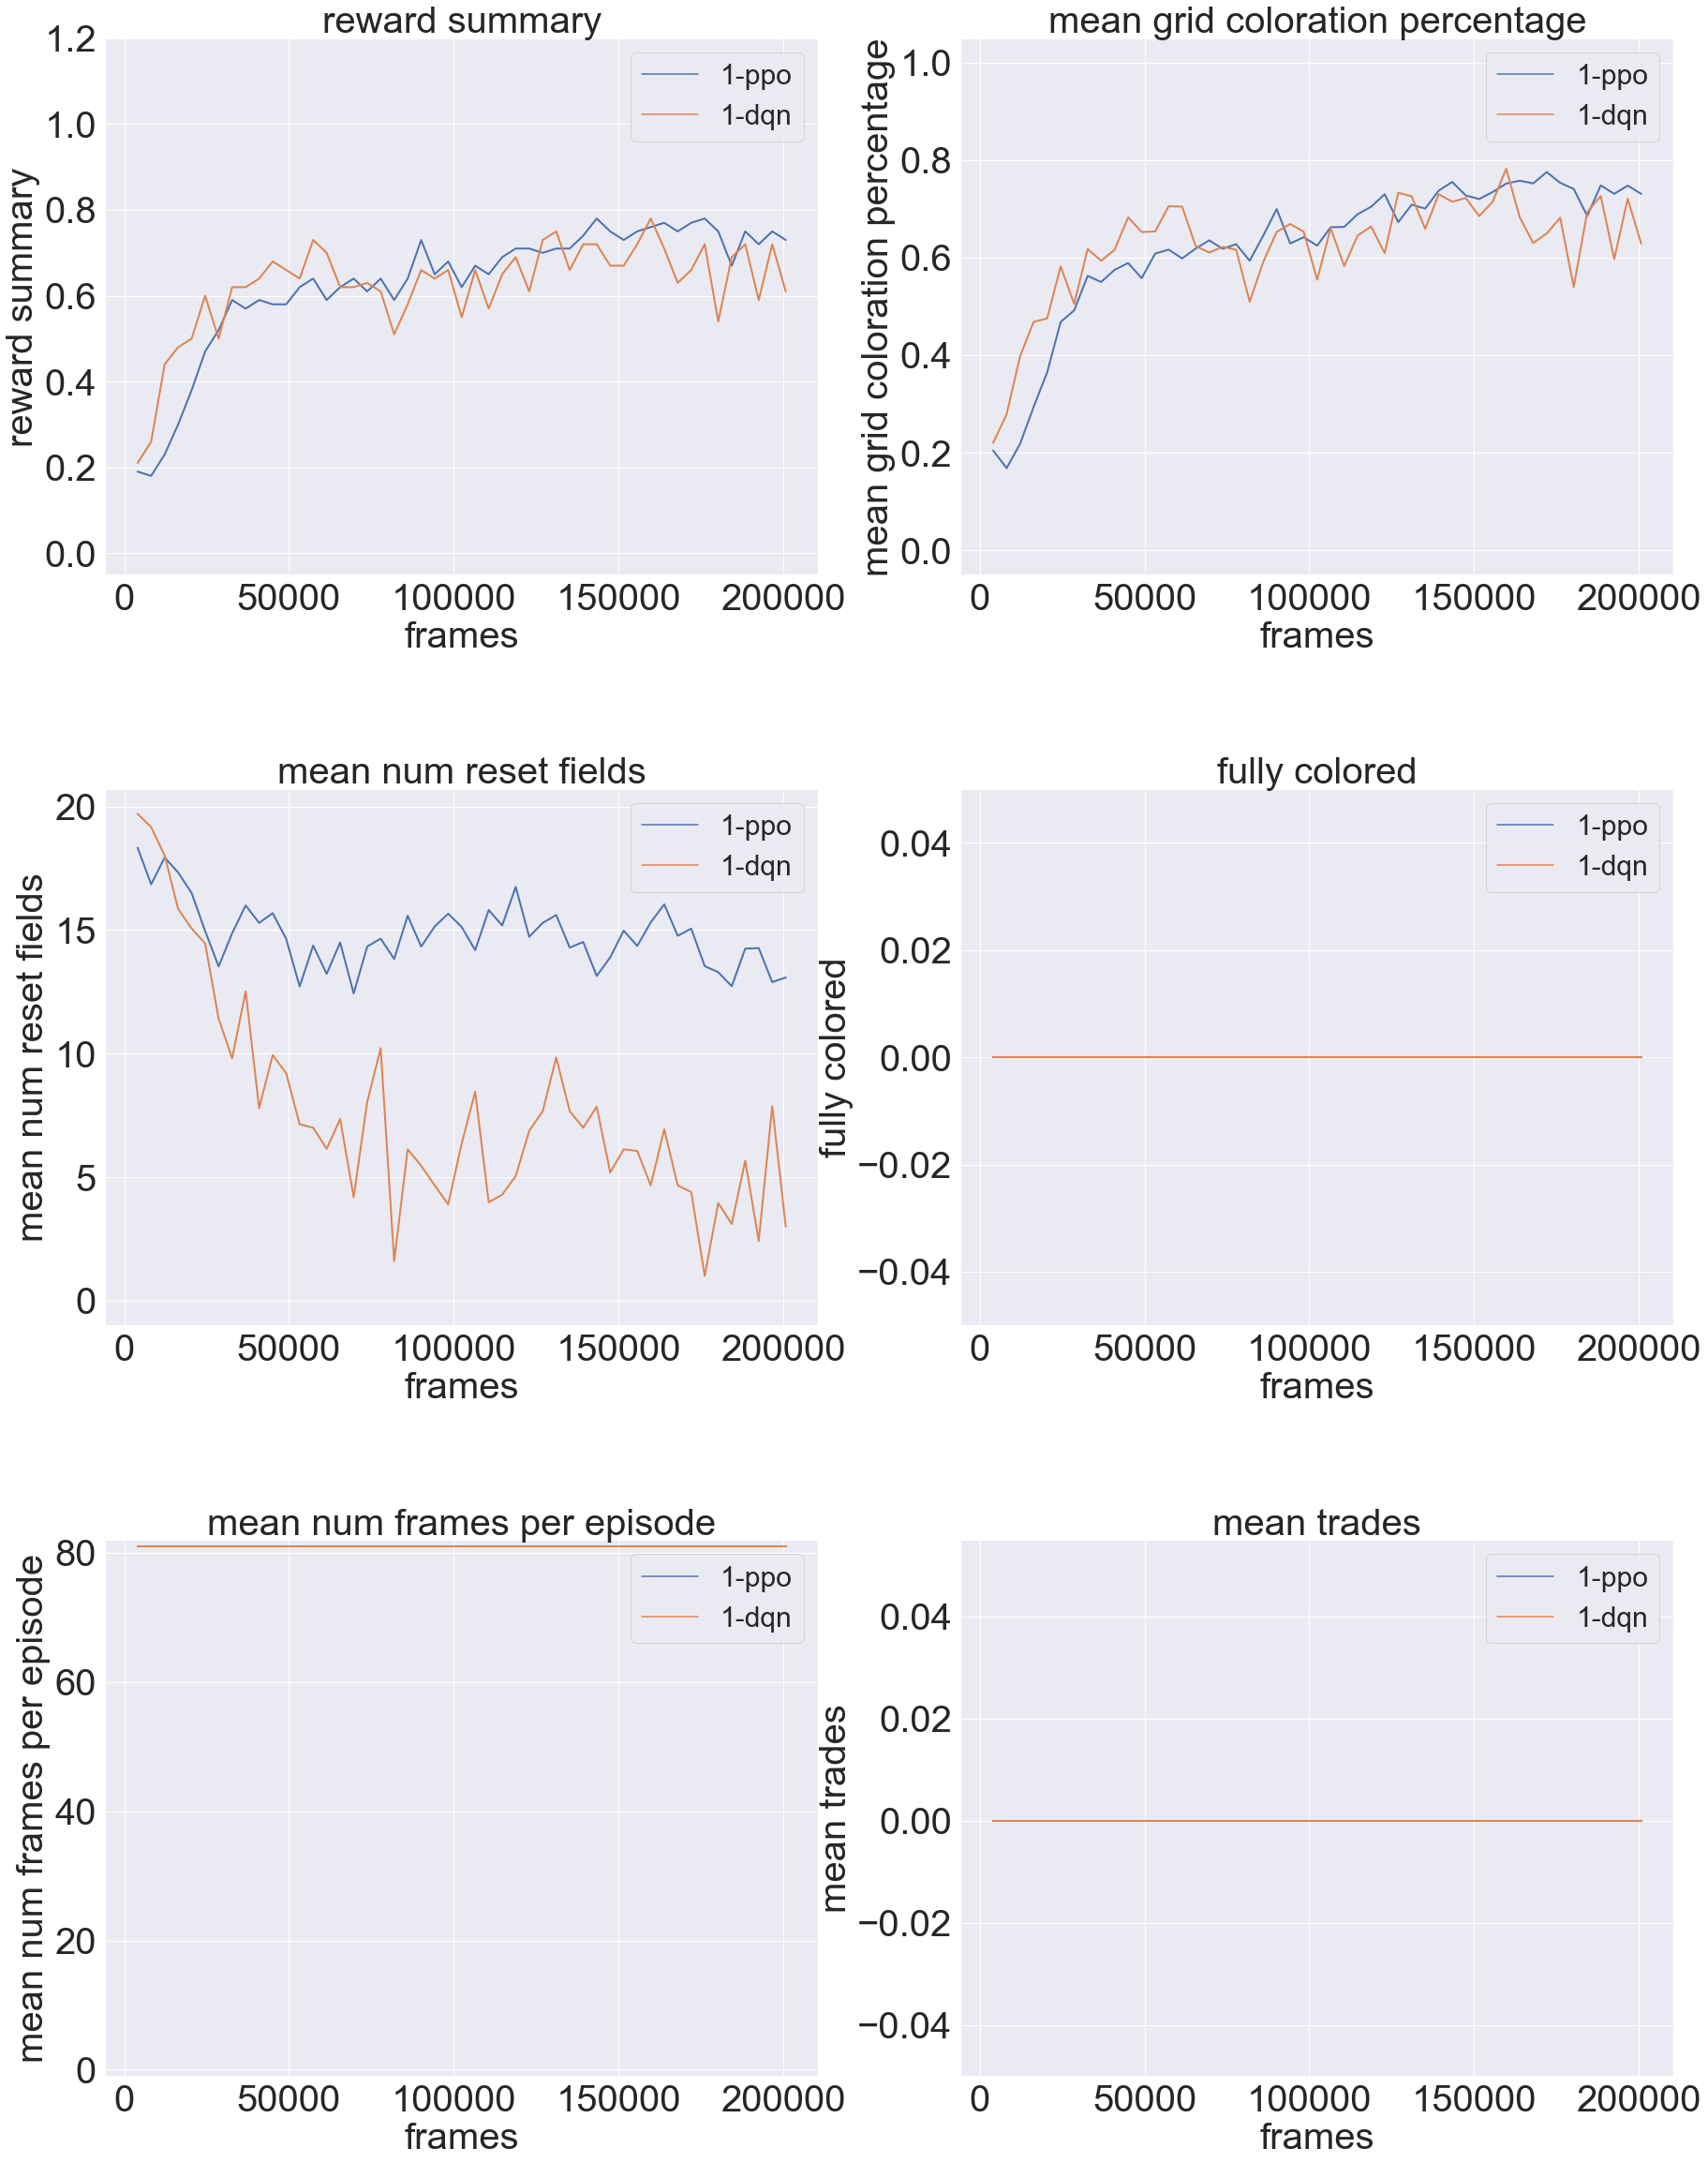
\includegraphics[width=1\textwidth]{AX-rooms-1.png}\\
    \caption[PPO and DQN Training Details with One Agent in a Rooms Environment]{Details of the training  in a 9x9 Rooms Environment with one agent using PPO and DQN}\label{fig:ax-rooms-1}
\end{figure}
\vfill
\clearpage


\newpage
\vfill
\begin{figure}
    \centering
    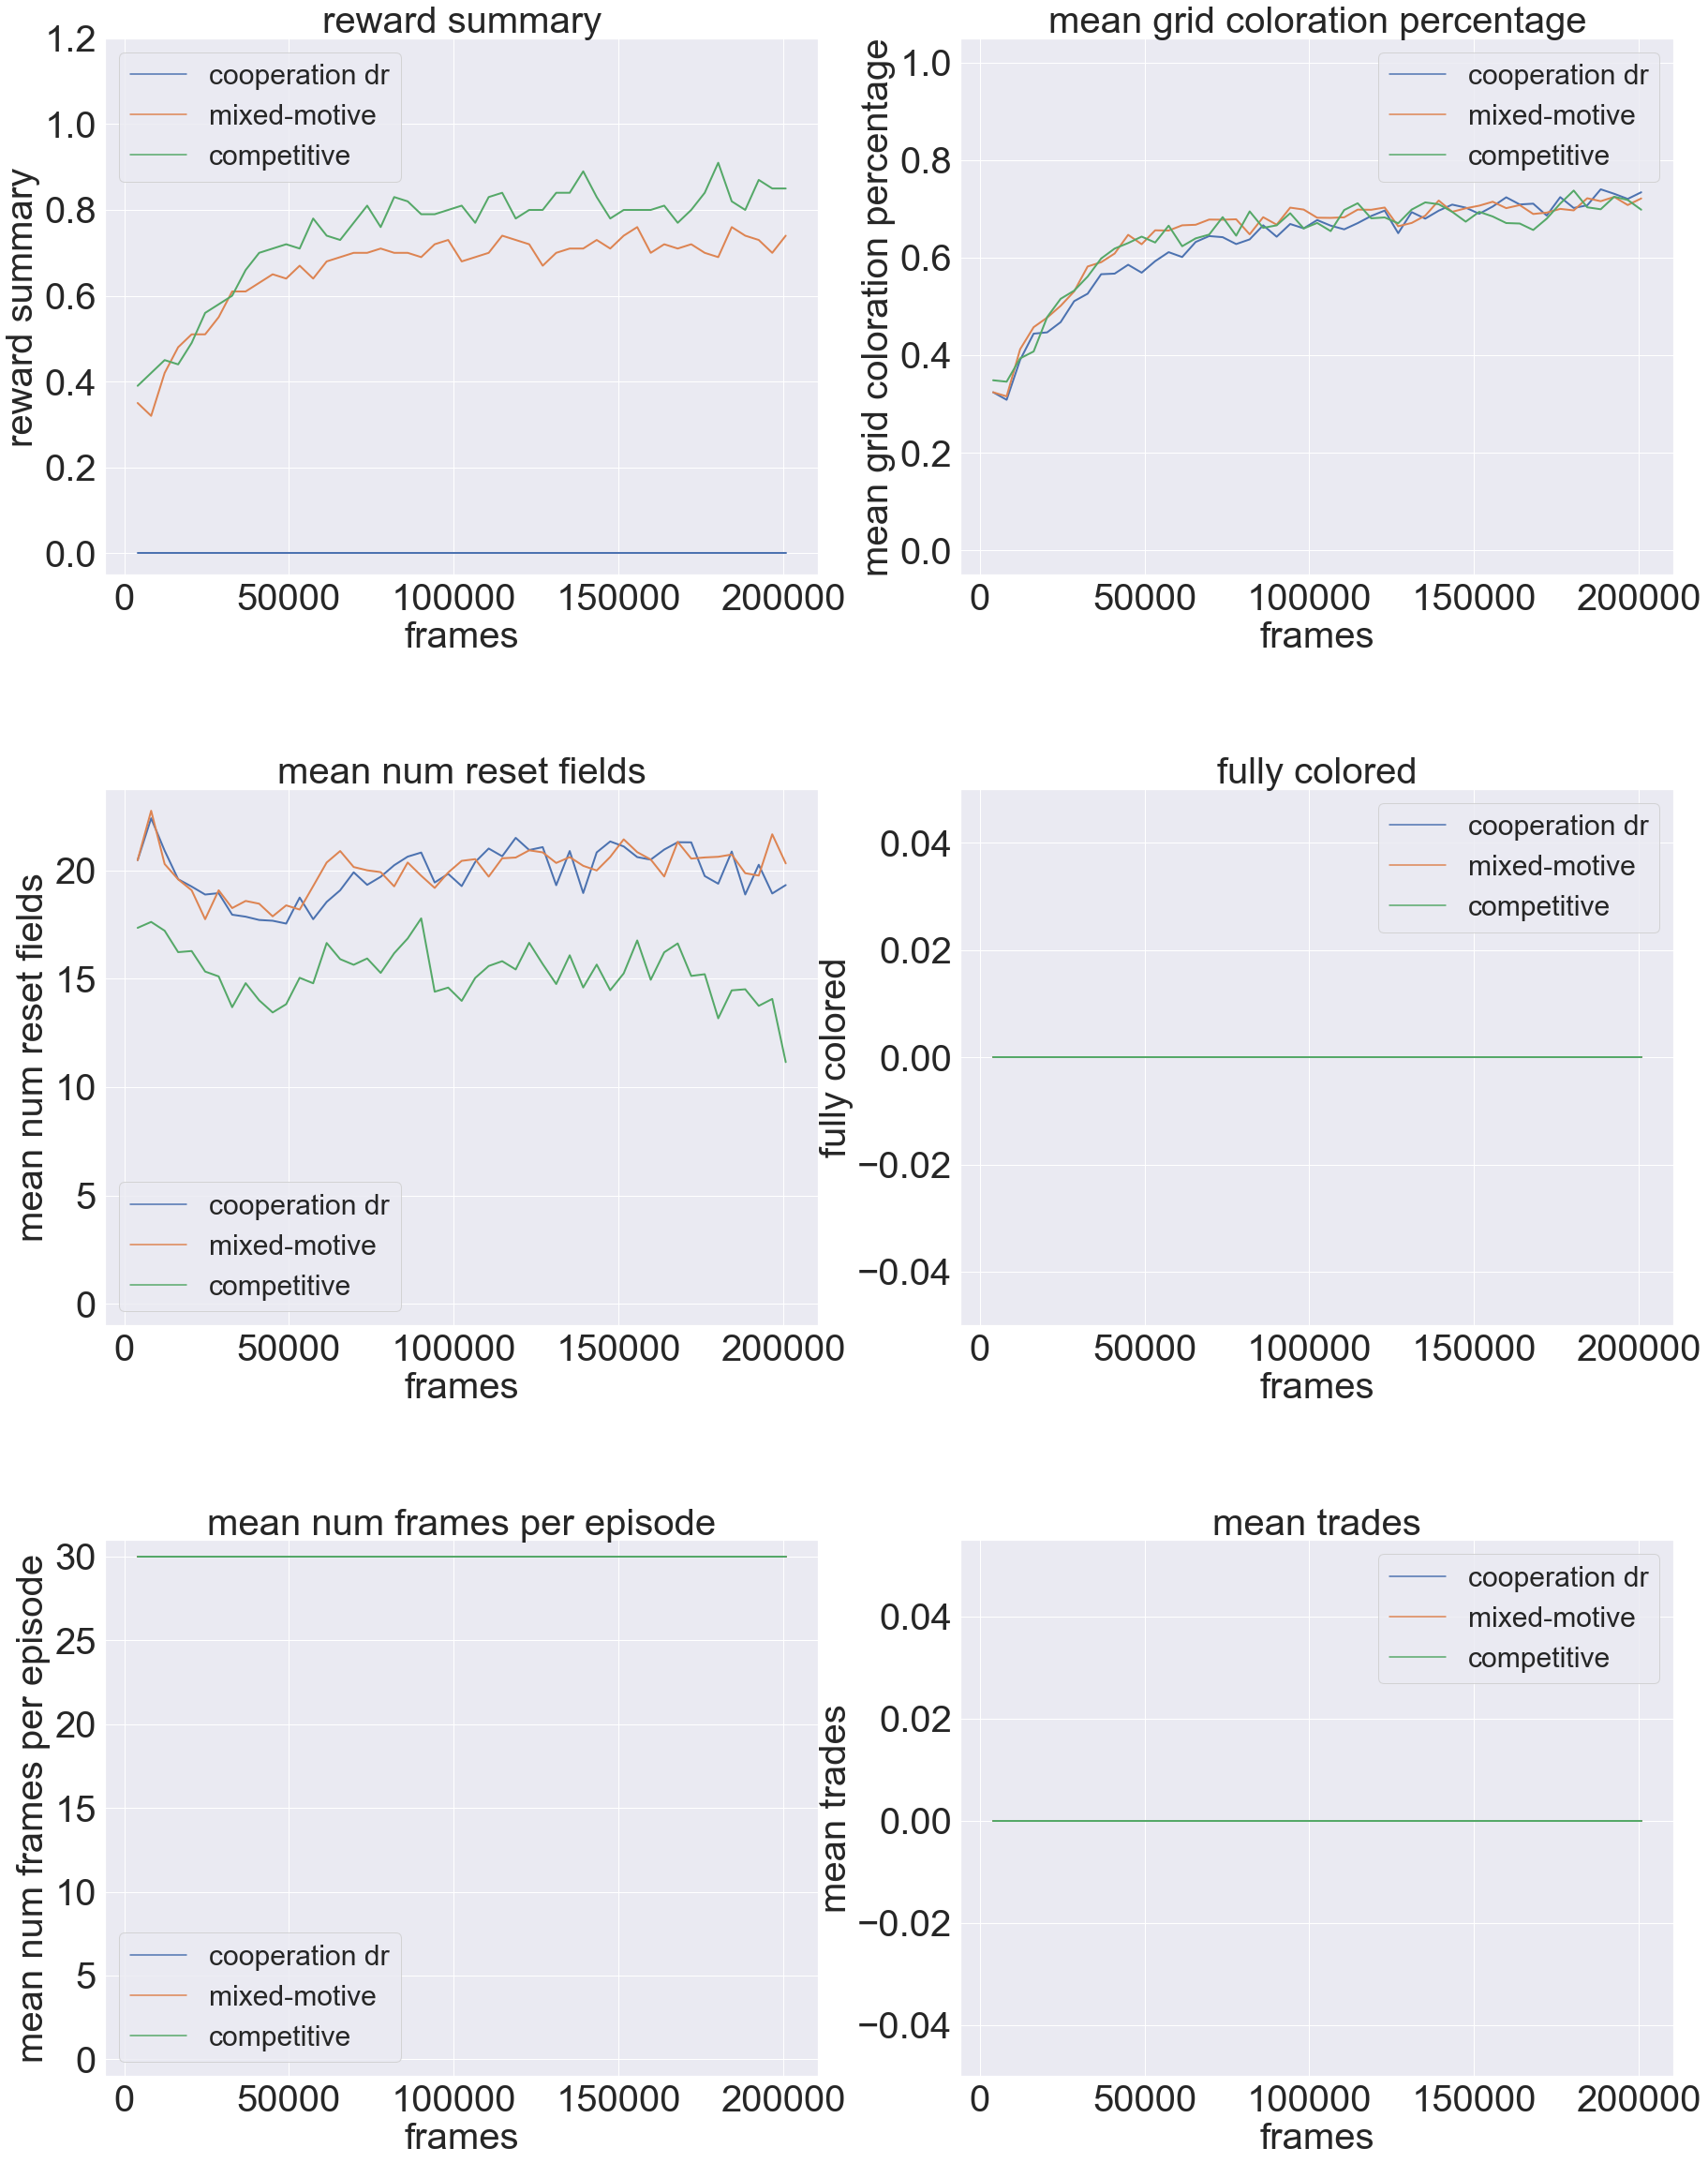
\includegraphics[width=1\textwidth]{AX-rooms-3-ppo.png}\\
    \caption[Training Details of Top PPO Competitive Executions in a Rooms Environment]{Top score details of three PPO agents in a 9x9 Rooms Environment}\label{fig:ax-rooms-3-ppo}
\end{figure}
\vfill
\clearpage


\newpage
\vfill
\begin{figure}
    \centering
    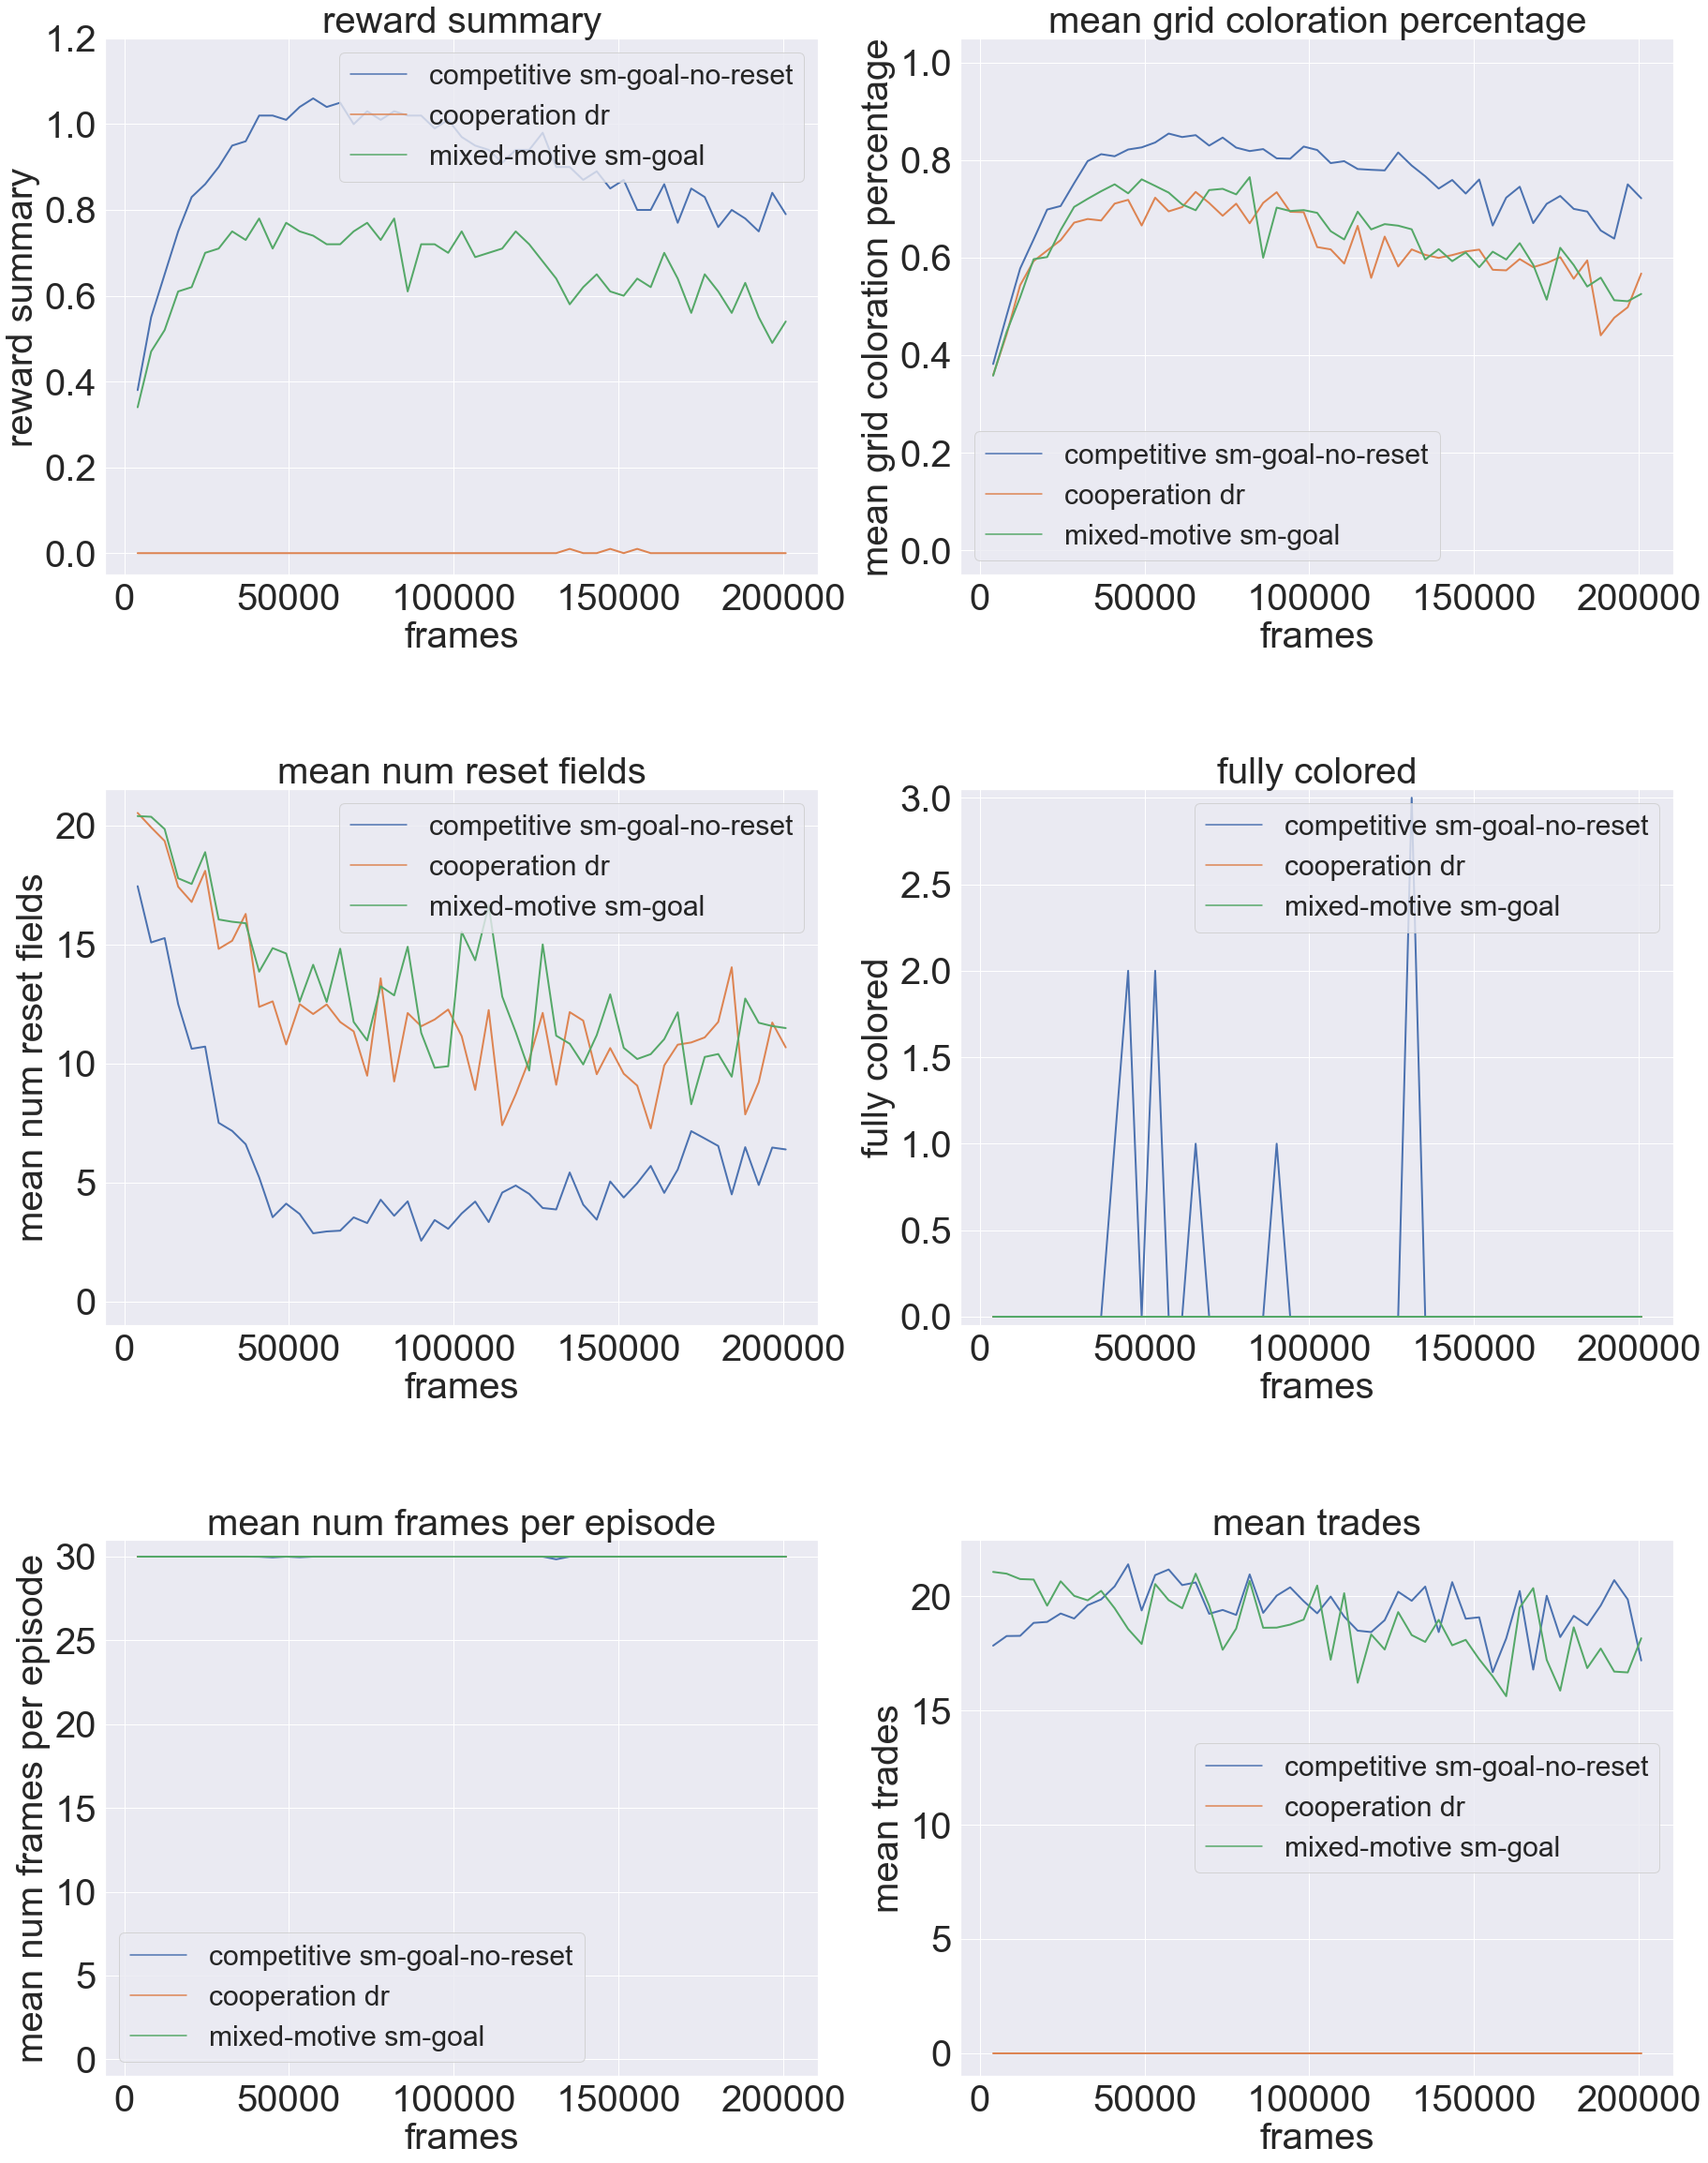
\includegraphics[width=1\textwidth]{AX-rooms-3-dqn.png}\\
    \caption[Training Details of Top DQN Competitive Executions in a Rooms Environment]{Top score details of three DQN agents in a 9x9 Rooms Environment}\label{fig:ax-rooms-3-dqn}
\end{figure}
\vfill
\clearpage

% further appendix
%
% =================================================================================================
% comment \listoffigures and/or \listoftables if not wanted
% -------------------------------------------------------------------------------------------------
%
\backmatter
\listoffigures                                % list of figures (uncomment if wanted)
\listoftables                                 % list of tables (uncomment if wanted)
\lstlistoflistings                            % list of listings (uncomment if wanted)
%
% =================================================================================================
% place your bibliography here
% -------------------------------------------------------------------------------------------------
%
\begin{spacing}{0.9}                          % save some space
    % \bibliographystyle{geralpha}               % for german thesis
    \bibliographystyle{alpha}                 % for english thesis
    \bibliography{bibliography}                % the location of bib file
\end{spacing}
\end{document}
%
% =================================================================================================
% end of document
% -------------------------------------------------------------------------------------------------
%
